\documentclass[a4paper,12pt]{report}

%%%%%%%%%%%%%%%%%%%%%%%%%%%%
% Universidad Gastón Dachary
%%%%%%%%%%%%%%%%%%%%%%%%%%%%
% Modification History
%
% Based on usthesis.cls by Jonathon Read
% http://www.cogs.susx.ac.uk/users/jlr24/latex.html
% Modified by Anthony Smith, Feb 2007
% Incorporated into single thesis.tex file, Anthony Smith, 30 June 2008
% Minor alterations to page numbering, AJS, 25 July 2008
% New alternative hyperref options for print version, AJS, 11 Sep 2008
% "DRAFT" on header, AJS, 12 Sep 2008
%%%%%%%%%%%%%%%%%%%%%%%%%%%%


%%%%%%%%%%%%%%%%%%%%%%%%%%%%
% LINE SPACING
\newcommand{\linespacing}{1.5}
\renewcommand{\baselinestretch}{\linespacing}
%%%%%%%%%%%%%%%%%%%%%%%%%%%%


%%%%%%%%%%%%%%%%%%%%%%%%%%%%
% BIBLIOGRAPHY STYLE
\bibliographystyle{unsrt}
%\bibliographystyle{plain} for [1], [2] etc.
%\bibliographystyle{apalike}
%%%%%%%%%%%%%%%%%%%%%%%%%%%%


%%%%%%%%%%%%%%%%%%%%%%%%%%%%
% OTHER FORMATTING/LAYOUT DECLARATIONS
% Graphics
\usepackage{graphicx,color}
\usepackage{epstopdf}
\usepackage[utf8]{inputenc}
\usepackage[spanish]{babel}
\usepackage{dirtytalk} % Permite el uso de say
\usepackage{csquotes}  % Permite el uso de \begin{displayquote} 

% The left-hand-side should be 40mm.  The top and bottom margins should be
% 25mm deep.  The right hand margin should be 20mm.
\usepackage[a4paper,top=2.5cm,bottom=2.5cm,left=4cm,right=2cm,headsep=10pt]{geometry}
\flushbottom
% Pages should be numbered consecutively thorugh the main text.  Page numbers
% should be located centrally at the top of the page.
\usepackage{fancyhdr}
\fancypagestyle{plain}{
	\fancyhf{}
	% Add "DRAFT: <today's date>" to header (comment out the following to remove)
	%\lhead{\textit{DRAFT: \today}}
	%
	%\chead{\thepage}
	\rhead{Tesis Josi Marcos}
    \cfoot{Página \thepage}
	\renewcommand{\headrulewidth}{0pt}
}
\pagestyle{plain}
%%%%%%%%%%%%%%%%%%%%%%%%%%%%


%%%%%%%%%%%%%%%%%%%%%%%%%%%%
% ANY OTHER DECLARATIONS HERE:

%%%%%%%%%%%%%%%%%%%%%%%%%%%%


%%%%%%%%%%%%%%%%%%%%%%%%%%%%
% HYPERREF
\usepackage[colorlinks,pagebackref,pdfusetitle,urlcolor=blue,citecolor=blue,linkcolor=blue,bookmarksnumbered,plainpages=false]{hyperref}
% For print version, use this instead:
%\usepackage[pdfusetitle,bookmarksnumbered,plainpages=false]{hyperref}
%\usepackage{backref}
%\renewcommand{\backrefpagesname}{Cited on}
%%%%%%%%%%%%%%%%%%%%%%%%%%%%


\usepackage[
backend=biber,
style=numeric,
sorting=none
]{biblatex}
\addbibresource{Referencias/bib.bib}



%%%%%%%%%%%%%%%%%%%%%%%%%%%%
% BEGIN DOCUMENT
\begin{document}
%%%%%%%%%%%%%%%%%%%%%%%%%%%%


%%%%%%%%%%%%%%%%%%%%%%%%%%%%
% PREAMBLE: roman page numbering i, ii, iii, ...
%\pagenumbering{roman}
%%%%%%%%%%%%%%%%%%%%%%%%%%%%


%%%%%%%%%%%%%%%%%%%%%%%%%%%%
%% TITLE PAGE: The title page should give the following information:
%%	(i) the full title of the thesis and the sub-title if any;
%%	(ii) the full name of the author;
%%	(iii) the qualification aimed for;
%%	(iv) the name of the University of Sussex;
%%	(v) the month and year of submission.
\thispagestyle{empty}
\begin{flushright}

\includegraphics[width=7cm]{Img/ugdlogo.jpg}
\end{flushright}	
\vskip40mm
\begin{center}
% TITLE
\huge\textbf{COCADA}
\vskip2mm
% SUBTITLE (optional)
\large\textit{Aplicación web para revisiones de modelos 3D paramétricos con un enfoque LEAN UX y Agile}
\vskip5mm
% AUTHOR
\Large\textbf{José María Guaimas, Marcos Daniel Henning}
\vskip5mm
% Director
\Large\textbf{Director: Ing. Juan B. Cabral}\\
\Large\textbf{Co-Director: Ing. Héctor Ruidiaz}
\normalsize
\end{center}
\vfill
\begin{flushright}
\large
% QUALIFICATION
Departamento de Informática \\
Universidad Gastón Dachary 2018\\
% DATE OF SUBMISSION

\end{flushright}		
%%%%%%%%%%%%%%%%%%%%%%%%%%%%


%%%%%%%%%%%%%%%%%%%%%%%%%%%%
% DECLARATIONS
%\chapter*{Declaration}
%I hereby declare that this thesis has not been and will not be submitted in whole or in part to another University for the award of any other degree.
	
% ADDITIONAL DECLARATIONS HERE (IF ANY)

%\vskip5mm
%Signature:
%\vskip20mm
% AUTHOR
%José María Guaimas
%%%%%%%%%%%%%%%%%%%%%%%%%%%%


%%%%%%%%%%%%%%%%%%%%%%%%%%%%
% SUMMARY PAGE
\thispagestyle{empty}
\newpage
\null\vskip10mm
\begin{center}
\large
\underline{Universidad Gastón Dachary}
\vskip20mm
% AUTHOR, QUALIFICATION
\textsc{José María Guaimas, Marcos Daniel Henning}\\
\textsc{Ingeniería en Informática}
\vskip20mm
% TITLE
\underline{\textsc{Título de la Tesis}}
\vskip0mm
% SUBTITLE (optional)
\underline{\textsc{Subtítulo}}
\vskip20mm
%\underline{\textsc{Sumario}}%
\vskip2mm
\end{center}
% Change line spacing
\renewcommand{\baselinestretch}{1.0}
\small\normalsize
% SUMMARY HERE (300 word limit for most subjects):

\thispagestyle{empty}
%%%%%%%%%%%%%%%%%%%%%%%%%%%%


%%%%%%%%%%%%%%%%%%%%%%%%%%%%
% ACKNOWLEDGEMENTS
\chapter*{Agradecimientos}
\renewcommand{\baselinestretch}{\linespacing}
\small\normalsize
% ACKNOWLEDGEMENTS HERE:

\thispagestyle{empty}
%%%%%%%%%%%%%%%%%%%%%%%%%%%%


%%%%%%%%%%%%%%%%%%%%%%%%%%%%
% TABLE OF CONTENTS, LISTS OF TABLES & FIGURES
\newpage
\pdfbookmark[0]{Contents}{contents_bookmark}
\tableofcontents
%\listoftables
%\phantomsection
%\addcontentsline{toc}{chapter}{List of Tables}
%\listoffigures
%\phantomsection
%\addcontentsline{toc}{chapter}{List of Figures}
%%%%%%%%%%%%%%%%%%%%%%%%%%%%

\thispagestyle{empty}
%%%%%%%%%%%%%%%%%%%%%%%%%%%%
% MAIN THESIS TEXT: arabic page numbering 1, 2, 3, ...
\newpage
\pagenumbering{arabic}
%%%%%%%%%%%%%%%%%%%%%%%%%%%%


%%%%%%%%%%%%%%%%%%%%%%%%%%%%
% RESUMEN
% ADDITIONAL DECLARATIONS HERE (IF ANY)

%\vskip5mm
%Signature:
%\vskip20mm
%AUTOR
%José María Guaimas



%-----------------------------------------------------
% Resúmen 2
%-----------------------------------------------------
\addcontentsline{toc}{section}{Resúmen}
\section*{Resúmen}
En el pasado el proceso de fabricar un producto consistía en delegar el diseño o enviar planos a un especialista para que realice la manufactura, los contactos eran presenciales y mantener el proyecto bajo control obligaba a realizar viajes frecuentes. 

En la actualidad el contexto es muy diferente: El Desarrollo Colaborativo de Productos y el Co-Diseño son conceptos muy utilizados en las organizaciones, en especial, en las áreas que involucran el diseño y fabricación asistido por computadora usando técnicas CAD/CAM. Gracias a la evolución de las tecnologías web se asume la colaboración entre personas dispersas geográficamente, de diferentes campos de especialización e incluso sin formación en diseño. \vskip
Al mismo tiempo, la diversidad de conocimientos trae como consecuencia algunos problemas en la gestión de los proyectos, entre ellos: la comunicación imprecisa entre los participantes, la múltiple interpretación de ideas y la complejidad en el registro de cambios en los diseños. 

El presente trabajo propone el diseño e implementación de un prototipo de aplicación web que permite la colaboración multidisciplinaria mediante revisiones de modelos 3D, estableciendo una comunicación fluída entre los participantes que vaya más allá de la geometría. 

El prototipo llamado \textit{Colaborative CAD Application} (COCADA) utiliza el enfoque LEAN UX combinado con metodologías ágiles de desarrollo de software y el uso de tecnologías web \textit{Free Libre Open Source Software} (FLOSS)\footnote{\url{https://es.wikipedia.org/wiki/Software\_libre\_y\_de\_c\%C3\%B3digo_abierto}}. \vskip
 \vskip
El software COCADA se encuentra disponible para la descarga en \url{https://github.com/jositux/Tesis_Josi_Marcos}  bajo licencia GNU General Public License (GPL)\footnote{\url{https://www.gnu.org/licenses/gpl-3.0.en.html}}. 

\vskip5mm
Palabras Claves: Diseño Colaborativo, CPD, OpenJSCAD, Javascript, Vue.js, Node.js, LEAN UX, Agile




	
% ADDITIONAL DECLARATIONS HERE (IF ANY)

%\vskip5mm
%Signature:
%\vskip20mm
%AUTOR
%José María Guaimas
%%%%%%%%%%%%%%%%%%%%%%%%%%%%


%%%%%%%%%%%%%%%%%%%%%%%%%%%%
% CAPITULOS
% Mantenemos los capítulos separados.
% Dentro de la carpeta archivo nuevo el nombre correspondiente X.tex"
% Agregamos de la siguiente manera y para no mostrar usamos el porcentual %:

%-----------------------------------------------------
% Chapter 1: Introducción
%-----------------------------------------------------
\chapter{Introducción}
\label{chap:cap1}

%This is the introduction to the %thesis.\footnote{And this is a %footnote.}  The conclusion is in %Chapter \ref{chap:cap1} on page %\pageref{chap:cap1}.

\section{Conceptos Preliminares}
%Figure \ref{us_figure} shows the logo for the %University of Sussex.\footnote{This is a URL: %\url{http://www.sussex.ac.uk}} This is %consistent with Special Relativity %\citep{Einstein1905}. $E=mc^2$.

%\begin{figure}
%\centering
%
\includegraphics[width=5cm]{uslogo}
%\caption[US Logo (optional short %caption)]{\label{us_figure} The logo for the %University of Sussex.}
%\end{figure}

La fabricación digital es una realidad gracias a la masificación de la tecnologías basadas en Control Numérico Computarizado (CNC) \footnote{ https://es.wikipedia.org/wiki/Control\_numérico } 
en combinación con técnicas de Diseño Asistido por Computadora y  Fabricación Asistida por Computadora en inglés  \textit{Computer-Aided Design/Computer-Aided Manufacturing} (CAD/CAM) \footnote{ https://es.wikipedia.org/wiki/CAD/CAM}, se pueden aplicar a casi cualquier caso de manufactura. Sus aplicaciones son muy variadas: desde prototipos de productos en plástico a la fabricación robótica de prótesis dentales. \vskip

Conceptos como \textit{Collaborative Product Development} (CPD) \footnote{ https://en.wikipedia.org/wiki/Collaborative\_product\_development } hacen posible la participación de ingenieros, diseñadores industriales, arquitectos, programadores, artistas e incluso personas sin formación específica, generando nuevas técnicas de diseño y procedimientos de fabricación innovadores.
Este escenario es conocido como co-diseño o diseño colaborativo, el cuál puede definirse como \say{un proceso de colaboración creativa entre diseñadores y personas, los cuáles no poseen una formación previa en diseño, con el propósito de resolver
problemas significativos.\cite{PerezGarcia2014}}. \vskip

Las nuevas tendencias en la tecnología han ayudado a democratizar la creatividad y la participación en
el diseño, en muchos niveles. Los teléfonos inteligentes son un ejemplo de la tecnología al
servicio de todas las personas, porque ofrecen oportunidades para la co-creación mediante
sus aplicaciones.\cite{Dr.EduardoHuerta2013}
\vskip
El contenido compartido en los entornos de diseño colaborativos por lo general implica el uso de modelos 3D como medios de comunicación entre los participantes con el fin de visualizar ideas abstractas y se usan iterativamente durante todo el proceso de diseño. Además, para permitir la participación es necesario contar un repositorio común de datos además de la geometría, incluyendo especificaciones y documentos en diferentes formatos según las particularidades de cada proyecto.\cite{Tek-JinNam2009}
\vskip
La revisión del diseño es una etapa fundamental para el control de calidad porque permite evaluar la capacidad de los resultados obtenidos para cumplir los requisitos, identificar cualquier problema y proponer soluciones. Los resultados de las revisiones deben ser registrados, lo más habitual es registrar estos resultados en actas de reunión o bien en algún formato de cláusula o contrato que se haya diseñado específicamente para controlar el diseño. 
\footnote{ http://www.portalcalidad.com/articulos/52-diseno_productos_iso_9001 } 

Para satisfacer a los participantes en el proceso de revisión, el enfoque LEAN UX \cite{Gothelf2013} propone principios básicos inspirados en las metodologías ágiles de desarrollo de software, uno de ellos explica que la colaboración entre los participantes es más importante que la negociación de contratos. Si las decisiones se toman por consenso se obtiene como resultado iteraciones más rápidas y una verdadera implicación de todos en el diseño.

En los siguientes capítulos, se define el proceso de creación de una herramienta tecnológica que soporta el co-diseño, utilizando metodologías de diseño y desarrollo de software con un enfoque acorde a los principios colaborativos planteados. \vskip


\section{Objetivos}
\subsection {Objetivo General}
Diseñar e implementar un prototipo de software colaborativo multiplataforma para revisiones de modelos 3D paramétricos.

\subsection {Objetivos Específicos}
\begin{itemize}
  \item Describir el estado actual de la tecnologías colaborativas para el diseño iterativo de modelos 3D.
  \item Analizar y describir las tecnologías web disponibles para la visualización y manipulación directa de modelos 3D.
  \item Diseñar una Interfaz Gráfica de Usuario (GUI) de un entorno colaborativo basándose en el diseño de experiencia de usuario UX con el enfoque LEAN UX.
  \item Diseñar un modelo de dominio de una capa de servicios utilizando BDD (Desarrollo guiado por comportamiento) como metodología ágil.
  \item Determinar los requerimientos de software necesarios para diseñar el entorno colaborativo que permita la revisión de modelos 3D y genere archivos preparados para la fabricación digital.
  \item Desarrollar un prototipo de software con herramientas FLOSS según los requerimientos de la GUI y el Modelo de dominio.
  \item Probar el prototipo con usuarios finales en dos escenarios diferentes y evaluar los resultados.
\end{itemize}






%-----------------------------------------------------
% Chapter 2: Características
%-----------------------------------------------------
\chapter{Marco teórico}
\label{chap: cap2}
\section{Desarrollo Colaborativo de Productos (CPD)}

La complejidad creciente de los productos, así como la personalización de los mismos a las particularidades de cada cliente, hace necesaria la participación de especialistas para acortar los ciclos de desarrollo de producto y de puesta en el mercado. Tradicionalmente se consideraba la figura de ``contratistas", a los que se entregaban los planos para que construyeran las distintas partes que integran un proyecto de cualquier sistema. Los contactos se producían de forma presencial y obligaban a frecuentes viajes para mantener el proyecto bajo control  \citep{Ruiz}. \vskip
El concepto teórico de CPD como lo conocemos hoy en día tuvo su primer aparición en 1994 en el artículo ``Multimedia Comes of Age"\footnote{\url{https://books.google.com.ar/books?id=bw0AAAAAMBAJ}} de Peter Cassidy para la revista CIO. Sin embargo, la colaboración en el desarrollo de productos tiene antecedentes anteriores en el libro ``The sources of innovation" de Eric Von Hippel \citep{VonHippel1988}. En 1995 apareció en más publicaciones como "Complexities of Collaborative Product Development" de Margaret Bruce, Fiona Leverick y Dale Littler \citep{Complex1995}, durante esa época se analizaba sobre la relación entre compradores y proveedores, la complejidad misma del CPD y sus factores de éxito. Posteriormente, la temática fue apareciendo con más frecuencia en artículos periodísticos y presentaciones de papers en todo el mundo. Obviamente esto no excluye la posibilidad de existencia de conceptos anteriores similares o equivalentes. 


\subsection{Definiciones sobre el CPD}
En 1995, Bruce, Leverick y Littler describieron la visión de CPD como un medio efectivo para reducir el tiempo de desarrollo y el riesgo organizacional. Además declararon que el desarrollo colaborativo de productos es una proceso evolutivo y cómo la forma, el alcance de su iniciación y la continuación pueden cambiar en el tiempo \citep{Complex1995}. 

El CPD está definido por la Asociación de gestión de desarrollo de productos en inglés \textit{Product Development Management Association} (PDMA) \footnote{\url{http://www.pdma.org/}} desde 1996 como: \textquote{... cuando dos o más empresas deciden colaborar en el desarrollo de productos como socios mutuos, y esto difiere del concepto de externalización por el nivel de asociatividad, ya que las empresas colaboradoras están vinculadas en el proceso de entregar la solución final al cliente o al usuario}. \vskip

Si bien con esta definición se puede comprender al CPD como colaboración entre agentes externos, hay otras como la de R. Del Rosario en el 2003 que lo describe como \textquote{\textit{la aplicación de prácticas de colaboración en equipo a los esfuerzos de desarrollo de productos dentro de una organización y además abarca la concurrencia, la atención al ciclo de vida, los proveedores y la tecnología de información en un entorno centrado en el cliente}} \citep{Mesbah2007}.

Con respecto a la toma de desiciones, Marija Jankovic describe las implicaciones del contexto industrial colaborativo moderno durante el proceso de desarrollo del producto: \textquote{\textit{En este proceso, cada actor tiene objetivos definidos para su dominio de acción. Por lo tanto, la toma de decisiones en colaboración es un proceso donde los actores tienen objetivos diferentes y a menudo contradictorios. Los actores en el proceso colaborativo de toma de decisiones tienen también diferentes grados de conocimientos sobre el problema, así como diferentes informaciones y puntos de vista}} \citep{Marija2006}.

En este trabajo el concepto de CPD no se usa específicamente para la colaboración externa o interna de una empresa, sino que incluye elementos de colaboración y toma de decisiones entre personas independientemente de la organización a la que pertenece, por ejemplo: la colaboración para diseñar un producto entre un diseñador industrial y una persona sin formación específica como puede ser un emprendedor.\vskip

En este contexto, el diseño tiene una importancia fundamental, ya que incorpora la información que define todos los pasos hasta la elaboración final del producto. Puede decirse que la máxima eficacia se logra mediante la adecuación de esta etapa y es lo que realmente influye en el resultado final del producto.\vskip 

\subsection{Diseño}
\textquote{ISO 9000:2000, la Norma que contiene el vocabulario de la Familia ISO 9000, define DISEÑO (Y DESARROLLO) como:
Conjunto de procesos que transforma los requisitos en características especificadas, o en la especificación de un producto, proceso, o sistema. Perdiendo un poco de rigor, \textit{Diseñar es crear o definir cómo debe ser algo que satisface nuestros requisitos. Se trata de idear algo que no existe, o que no sabemos que existe. Sabemos qué función debe cumplir “ese algo”, pero no cómo debe ser, necesitamos diseñarlo}.} \citep{Pereiro2005}


\subsection{Co-diseño}

La irrupción del diseño colaborativo como paradigma está cambiando el panorama de la práctica del diseño clásico porque está permitiendo la aparición de nuevos dominios de creatividad colectiva. 

\textquote{\textit{El \textbf{co-diseño} o diseño colaborativo se refiere a cómo se aplica la creatividad colectiva a través de toda la duración de un proceso de diseño}} \citep{Huerta2013}. El concepto ha surgido tanto como un efecto de la globalización como también gracias a que se considera una potencial herramienta con la cual enfocar el desarrollo de productos, en una industria que requiere nuevas tecnologías y procesos para abordar el diseño de artefactos cada vez más complejos y satisfacer de esta manera las altas expectativas de los clientes. 
\textit{El co-diseño es definido por el hecho de que la creatividad de los diseñadores se une a la de personas que tienen otros perfiles y trabajan juntas en el proceso de elaboración del diseño}.
En esta definición se plantean los dos elementos fundamentales que soportan el paradigma de diseño colaborativo:
\begin{itemize}
    \item \textbf{a) Nuevos perfiles}\vskip
En esta nueva forma de ver el diseño, al grupo habitual de trabajo se suman la iniciativa y la creatividad de otros perfiles que hasta ahora aportaban ideas generalmente como agentes externos: el investigador, el cliente y la persona que finalmente se beneficiará con el resultado del co-diseño (el usuario).
En el diseño colaborativo estos perfiles tienden a mezclarse: El usuario pasa a jugar un rol de ``experto en su experiencia” y puede aportar elementos de valor en la generación de conceptos e ideas en una etapa inicial de desarrollo. La labor del investigador, a partir de la experiencia del usuario, será proporcionar herramientas acertadas para recoger todos los datos que dicho perfil puede aportar y, a la vez, puede desempeñar un papel fundamental en dar forma a las ideas. De ahí la idea de que el investigador y el diseñador puede ser la misma persona.
\item \textbf{b) Objetivo en común}\vskip
La idea del objetivo compartido se plantea como una de las principales diferencias con respecto a los métodos tradicionales del diseño de productos o artefactos. Los métodos de diseño generalmente se planteaban para ser llevados a cabo por expertos que realizaban tareas individuales. Con el trabajo individual no era necesario compartir la visión del objetivo general del proceso de diseño. En cambio, el diseño colaborativo plantea que este punto es fundamental: Para que el equipo funcione correctamente necesita tener la visión del objetivo en común.

Lógicamente, después de apuntar las características principales del diseño colaborativo, se infiere que el rol del diseñador en el proceso debe cambiar necesariamente al incluir este nuevos socios creativos en un entorno que tradicionalmente le pertenecía.

\end{itemize}

\subsection{Fuzzy Front End}
La Figura \ref{fig:fuzzy} se muestra una representación simple del proceso de diseño. Se puede apreciar un gran y creciente énfasis en la parte delantera o de la izquierda, proceso llamado ``pre-diseño" \o el ``front end".
El Front End ``Difuso" en inglés  \textit{Fuzzy Front End} (FFE) suele denominarse de esa manera debido a la ambigüedad y la naturaleza caótica que lo caracterizan. Se puede definir en el diseño como \textit{el período comprendido entre el momento en que se examina por primera vez una idea y el momento en que se considera que esa idea está lista}\citep{schreiner}.

\begin{figure}
\centering
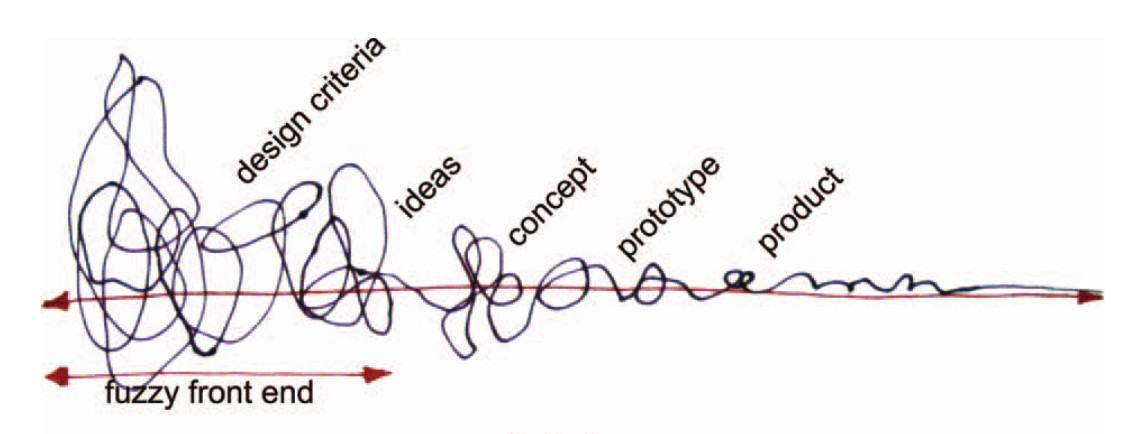
\includegraphics[width=12cm]{Img/CPD/cpd-fuzzy.jpg}
\caption[(optional short caption)]{\label{fig:fuzzy} Fuzzy Front End y proceso de diseño}
\end{figure}

\begin{figure}
\centering
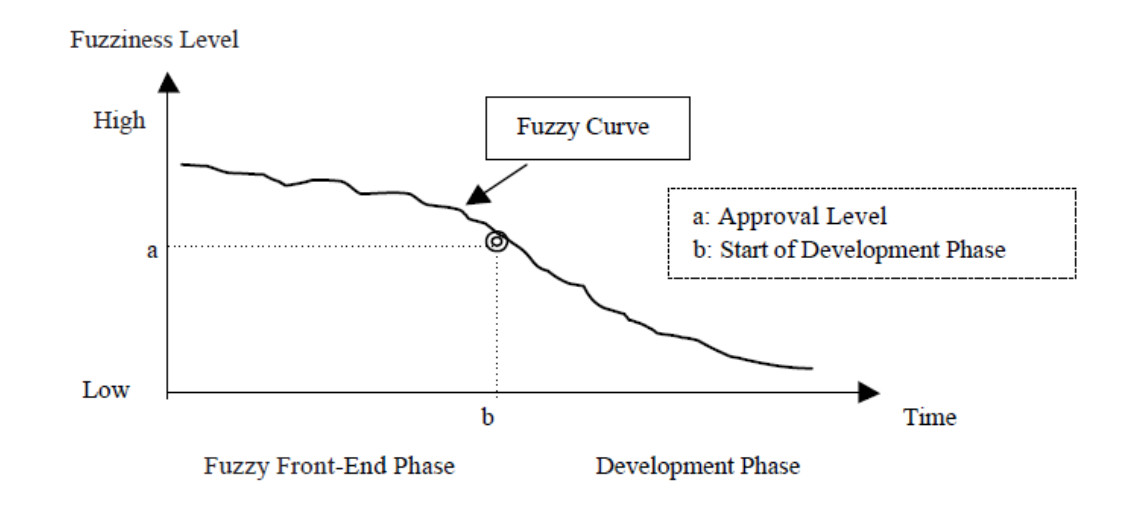
\includegraphics[width=12cm]{Img/CPD/cpd-fuzzi2.jpg}
\caption[(optional short caption)]{\label{fig:fuzzy} Fuzzy Front End y diseño de un producto}
\end{figure}

En el FFE, a menudo no se sabe si el resultado del proceso de diseño será un producto, un servicio, una interfaz, etc. Los puntos de vista de muchas fuentes se unen en esta fase cada vez más crítica, p. comprensión de los usuarios y contextos de uso, investigación y selección de oportunidades tecnológicas tales como nuevos materiales, tecnologías de la información, etc. El objetivo de las investigaciones es determinar qué se diseñará y, a veces, qué no se debe diseñar y fabricar. El FFE es seguido por los procesos de diseño clásico donde las ideas resultantes para el producto, servicio, interfaz, etc., se desarrollan primero en conceptos, y luego en prototipos que se perfeccionan sobre la base de los comentarios de los futuros usuarios.

Es una fase larga y poco comprendida, pero generalmente llena de oportunidades de mejora que pueden analizarse cuantitativamente y transformarse en beneficios para los proyectos. Las ideas difusas contienen elementos que pueden tener éxito o fallar y por lo tanto, esta fase necesita ser gestionada cuidadosamente. El prototipo de este trabajo de investigación pretende en cierta medida reducir el tiempo de esta etapa, brindando soporte a los participantes mediante herramientas tecnológicas. En la sección \ref{chap: cap3} de desarrollo se pueden ver las estrategias para lograrlo.



\begin{figure}
\centering
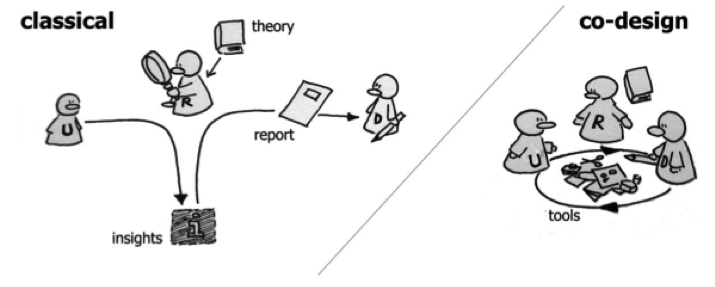
\includegraphics[width=12cm]{Img/CPD/1-CO.png}
\caption[(optional short caption)]{\label{us_figure} Diseño Clásico vs Co-diseño}
\end{figure}


\clearpage
\section{Diseño paramétrico} 
\label{disenoparam}

El término \textit{paramétrico} se originó en las matemáticas, pero hay un debate sobre cuándo comenzaron los diseñadores a usar la palabra, David Gerber en su tesis doctoral ``Parametric Practice'' acredita a Maurice Ruiter por usar el término en un trabajo de 1988 titulado ``Parametric Design''  \citep{Davis2013}. En 1987 la compañía Parametric Technology Corporation (PTC), fundada por el matemático Samuel Geisberg lanzó el primer software de modelado paramétrico con éxito comercial: Pro/ENGINEER \footnote{Pro/ENGINEER ahora conocido como Creo Elements/Pro, es un producto de diseño, fabricación e ingeniería asistida por computadora de PTC Corporation (Massachusetts. USA)}. Por su parte, Robert Stiles \citep{Davis2013} sostiene que la verdadera procedencia del término se produjo décadas antes en los escritos de los años 40 por el arquitecto italiano Luigi Moretti.\vskip
Moretti escribió extensamente sobre la arquitectura paramétrica, que define el estudio de los sistemas de arquitectura con el objetivo de \textit{definir las relaciones entre las dimensiones que dependen de los diversos parámetros}. En esa época usó el diseño de un estadio como un ejemplo, explicando cómo la forma del estadio puede derivar de diecinueve parámetros relacionados con aspectos como ángulos de visión y el costo económico del hormigón.\vskip 
Sin embargo, la parametrización tiene una larga historia en las matemáticas y los ejemplos más antiguos que se encontraron para describir modelos tridimensionales se producen mucho tiempo antes. Un ejemplo es el artículo de James Dana en 1837 llamado ``On the Drawing of Figures of Crystals" \citep{dana1838drawing}. En el documento, explica los pasos generales para dibujar una gama de cristales y las disposiciones para sus variaciones utilizando un lenguaje propio mezclado con parámetros, variables y proporciones.\vskip


\begin{figure}[h]
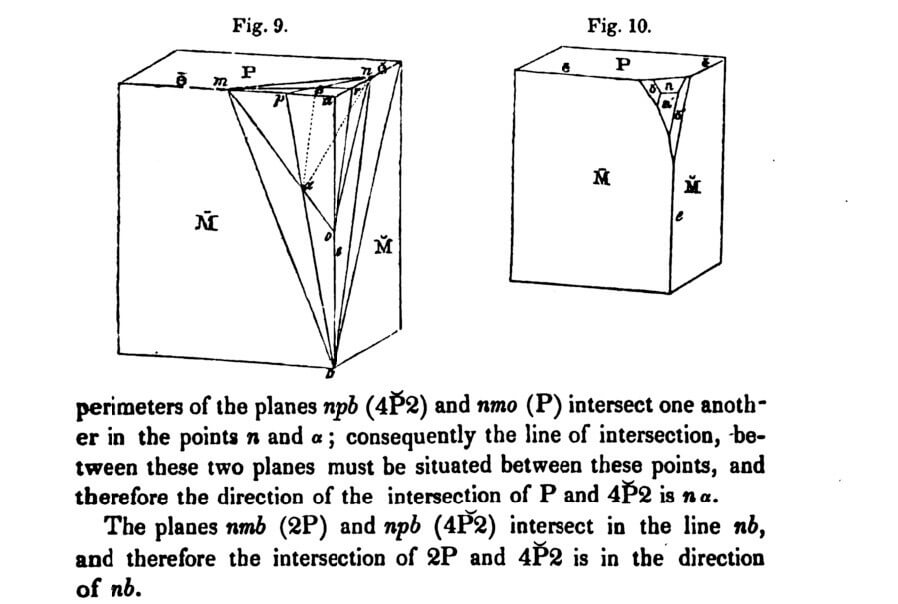
\includegraphics[width=12cm]{Img/GEO/geo-dana.jpg}
\centering
\caption{\textbf{\footnotesize{Definición de cristales por James Dana con un lenguaje propio}}}
\end{figure}


Existen muchos otros casos de ciencia del principio del siglo XIX involucrados con las matemáticas de representaciones paramétricas. Un ejemplo de esa época incluye a Sir John Leslie \footnote{John Leslie fué un físico y matemático escocés. Destacó principalmente en el estudio del calor. En 1804 inventó el cubo de Leslie, y en 1810 desarrolló el primer método de congelación artificial.}, en uno de sus libro sobre análisis geométrico, demostrando la auto-similitud de las curvas catenarias usando ``círculos paramétricos''. Otro ejemplo es Samuel Earnshaw. \footnote{Samuel Earnshaw fué un matemático y físico inglés, destacado por sus contribuciones a la física teórica, especialmente el Teorema de Earnshaw.} que escribió sobre ``superficies paramétricas hiperbólicas'' deformadas por líneas de fuerza en un documento que dio lugar al teorema de Earnshaw. Estos ejemplos de expresar la geometría con ecuaciones paramétricas son dos de muchos del período, un período mucho antes de que el arquitecto español Antoni Gaudí\footnote{Antoni Gaudí fué un arquitecto español, máximo representante del modernismo catalán con un sentido innato de la geometría y el volumen \url{http://www.antonigaudi.org/} } comenzara a diseñar arquitectura con curvas catenarias paramétricas y paraboloides hiperbólicos paramétricos a fines del siglo XIX.

Es imposible saber si Gaudí fue influenciado directamente por los científicos y matemáticos que anteriormente utilizaban ecuaciones paramétricas para definir geometrías. 
Mark Burry, el actual arquitecto ejecutivo de ``la Sagrada Familia" \footnote{El Templo Expiatorio de la Sagrada Familia, es una basílica católica de Barcelona, diseñada por el arquitecto Antoni Gaudí. Iniciada en 1882, todavía está en construcción.} explica que a pesar de que el currículum universitario de Gaudí incluía, entre otras cosas, matemáticas avanzadas, física general, ciencias naturales y geometría descriptiva ``prácticamente no hay nada escrito por él mismo sobre sus motivaciones, las teorías y las prácticas de su obra''. La comprensión de Gaudí sobre las matemáticas es la base de su arquitectura, especialmente en sus trabajos posteriores, que consiste en superficies diseñadas con helicoides, paraboloides e hiperboloides paramétricamente asociados con superficies regladas, booleanos, relaciones geométricas y arcos catenarios.

Mark Burry plantea que uno de los primeros ejemplos es la maqueta que utilizó el arquitecto para representar el modelo de la cripta de la Colonia Guell, a principios del siglo XX. Este modelo estaba compuesto por cadenas que sostenían pesos, y actuaban por la fuerza de la gravedad \citep{Kaled2016}.
La maqueta fue realizada al revés, y Gaudí le sacó una fotografía para poder visualizarla al derecho. Una cadena que cuelga tiene por lo menos cuatro parámetros: su longitud, su peso y los dos puntos a los que está sujetada. La cadena colgando a la merced de la fuerza de la gravedad adopta una forma curva. Esta curva es la función explicita de los parámetros de la cadena, con la propiedad agregada de que cuando es invertida la curva actúa por pura compresión. Al no haber una computadora, la cadena colgante es un modelo paramétrico gracias a la presencia de parámetros que controlan una forma derivada de una función explicita (en este caso, calculada por la gravedad). 


\begin{figure}[h]
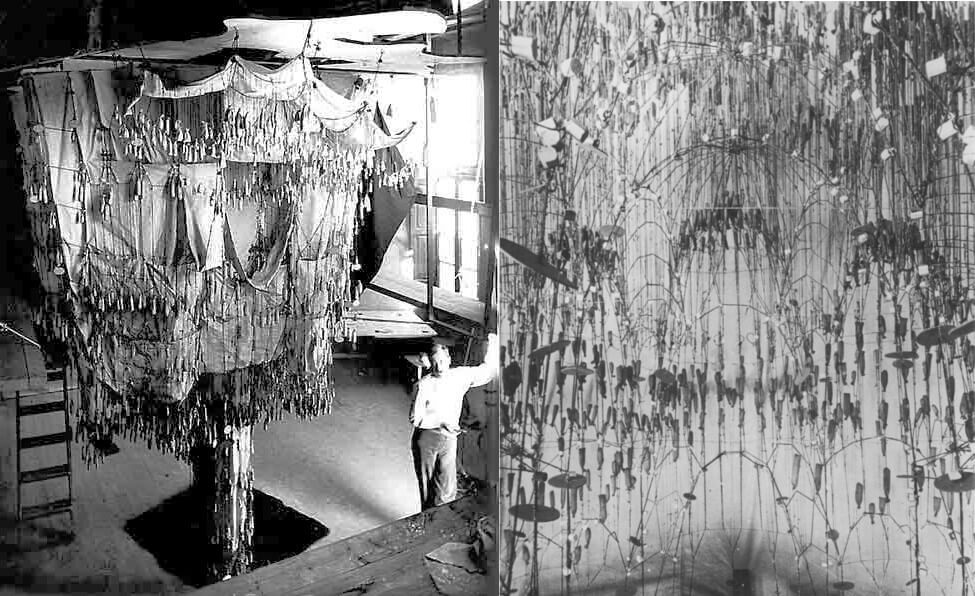
\includegraphics[width=12cm]{Img/GEO/geo-gaudic.jpg}
\centering
\caption{\textbf{\footnotesize{Maqueta gravitatoria y fotografía al revés donde se pueden apreciar los arcos catenarios.}}}
\label{fig:gaudi}
\end{figure}



\textquote{\textit{El \textbf{Diseño Paramétrico} se entiende en términos generales como un proceso de descripción de una problemática utilizando variables.}} Actualmente para describir estas variables, los diseñadores
insertan valores numéricos o algoritmos en un software especializado, al modificar las
variables se generan una serie de alternativas de soluciones, y según el criterio del diseñador, la solución final es creada. Davis y Hudson \citep{Kaled2016} coinciden en que \textit{el diseño paramétrico en su definición contemporánea es únicamente posible creando un \textbf{modelo paramétrico}}. Esto lo definen como un \textit{conjunto de ecuaciones que expresan una geometría explícitamente por medio de funciones definidas por parámetros}. Esta representación se basa en las relaciones entre estas variables. Todo sistema de esta índole está compuesto por unos parámetros iniciales y las relaciones entre ellos, de manera que si se ajusta uno de los parámetros, el resultado se verá afectado de manera acorde, al igual que si se altera alguna de las relaciones. Esto brinda una característica de fuerte y sencilla maleabilidad, que permite verificar resultados fácilmente. El diseñador que emplea estas herramientas en vez de diseñar un objeto resultante, se enfoca en crear lógicas que pongan en relación estos parámetros y resulten en un sistema vivo y ampliamente modificable de acuerdo a su criterio pero asistido por la computadora. El uso de este método por medio de la manipulación de los sistemas fomenta la exploración y la experimentación de las formas del producto, que se generan automáticamente por la modificación de los parámetros o las relaciones. Woodbury \citep{Kaled2016} afirma que \textit{el diseño es cambio y que el modelado paramétrico representa el cambio}. Esto lo menciona como una característica esencial del diseño paramétrico, como aquello que lo distingue de los métodos de diseño tradicionales. Es marcar e identificar las partes y como se relacionan y cambian de manera coordinada. La demostración explicita de las partes es lo que contribuye a la intervención y modificación interactiva en tiempo real, debido a la operatividad visible del cambio en el sistema. La lógica sistemática del diseño paramétrico permite evaluar las relaciones de manera visible, en lugar de hacerlo de manera intuitiva por medio de un proceso mental interno.
El diseñador puede explorar y descubrir nuevas posibilidades en lugar de explorar sus conocimientos previos para llegar con una solución que ya conocía.
El autor Nigel Cross \citep{Kaled2016} también afirma que es necesaria una representación visual ya que diseñar es difícil de conducir puramente por procesos mentales internos. En la Figura \ref{fig:procesopar} se puede analizar el proceso del diseño paramétrico.

\begin{figure}[h]
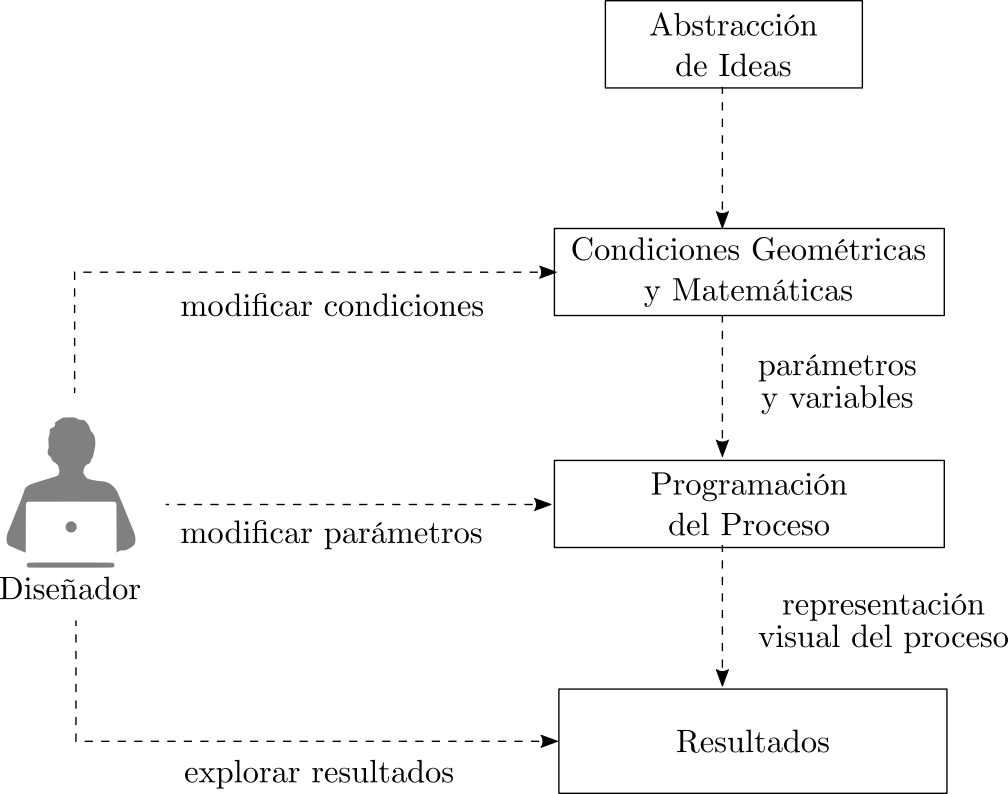
\includegraphics[width=12cm]{Img/CPD/diseno.png}
\centering
\caption{\textbf{\footnotesize{proceso de diseño paramétrico}}}
\label{fig:procesopar}
\end{figure}


\subsection{CAD Paramétrico}

Lo innovador del modelo de Gaudí, explicado la sección \ref{disenoparam} radica en que éste calcula automáticamente los resultados, porque que al mover un parámetro se afecta todo el modelo, que a pesar de ser análogo, marcó el inicio de la actualización en tiempo real de geometrías con bases matemáticas, lo cuál le da el énfasis utilitario de explorar las posibilidades que el modelo ofrece (ver Figura \ref{fig:gaudi}).
Esto marcó la \textit{necesidad de facilitar la interacción entre el diseñador y el modelo}, que implicaba muchas representaciones manuales y modificaciones completas con cada cambio. \vskip 
No fue hasta la aparición de las computadoras y el primer programa CAD, \textit{Sketchpad} de Ivan Sutherland en 1963 que se facilitó la interacción en tiempo real del diseñador y la computadora. Yüksel \citep{Kaled2016} lo describe como un sistema que tenía un puerto de entrada con un modelo de límites que promovía la interacción, porque al manipular una parte del modelo afectaría los cambios geométricos en otro. En el contexto de aparición de este programa, el proceso de diseño era enteramente manual y análogo, donde un cambio mínimo significaría comenzar de nuevo. Al representar las geometrías en dos dimensiones en la computadora se facilitaba el proceso de diseño. A partir de esto se fueron desarrollando un amplio número de software cuyas capacidades y posibilidades se extendían con aquellas del procesamiento de datos de las computadoras.\vskip
El recorrido histórico del desarrollo de software excede los objetivos de este trabajo final, pero la bifurcación entre la \textit{computarización del diseño} y el \textit{diseño computacional} es esencial para la compresión de los capítulos a seguir. Ambos términos suelen ser tomados como iguales, definidos como el uso de tecnologías CAD para realizar un proyecto de diseño. La diferencia radica en su empleo: la computarización del diseño apunta a el uso de la computadora como herramienta de dibujo o representación formal de un proyecto concebido en la mente del diseñador, mientras que \textit{el \textbf{diseño computacional} aborda el diseño con bases en el pensamiento algorítmico, lo que engloba al diseño paramétrico y generativo}. Esta diferenciación puede apreciarse claramente en el programa Sketchpad y el modelo de Gaudí. El programa de Sutherland representa geometrías modificables, mientras que la maqueta de Gaudí encarna un sistema complejo de parámetros y relaciones. \citep{Kaled2016}.

\begin{figure}[h]
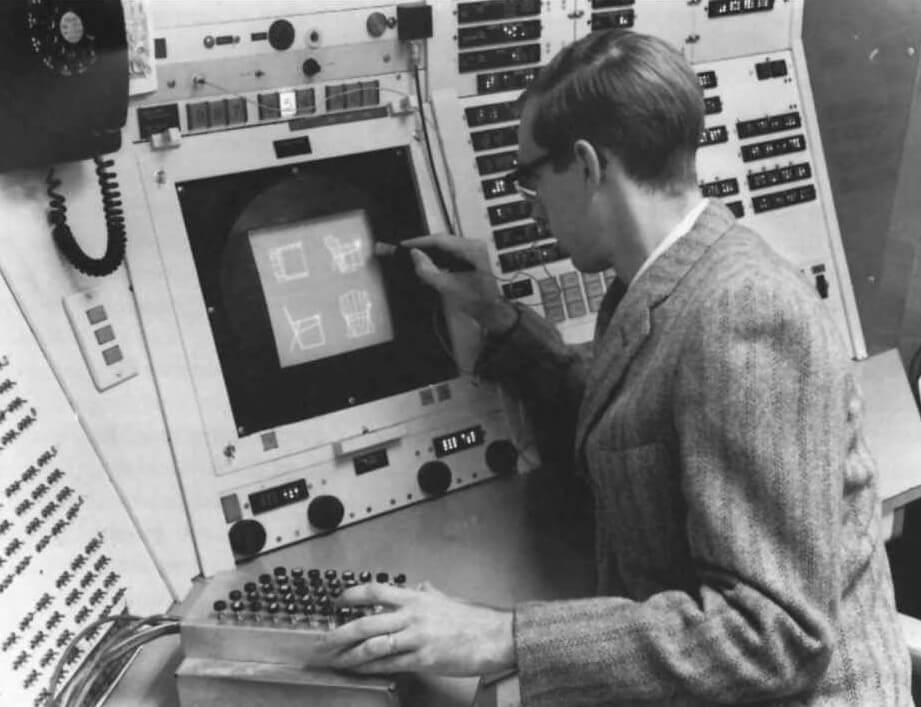
\includegraphics[width=8cm]{Img/GEO/geo-sketchpadc.jpg}
\centering
\caption{\textbf{\footnotesize{Ivan Sutherland utilizando sketchpad en 1962}}}
\end{figure}


Un ejemplo de software paramétrico masivamente utilizado es FreeCAD\footnote{\url{https://www.freecadweb.org/}}, una aplicación FLOSS de CAD 3D e ingeniería asistida por computadora muy utilizada en el diseño de elementos mecánicos. Utiliza técnicas de modelado paramétrico y está provisto de una arquitectura de software modular, permitiendo añadir funcionalidades mediante el lenguaje python\footnote{\url{https://www.python.org/}} sin tener que cambiar el núcleo del sistema.

\begin{figure}[h]
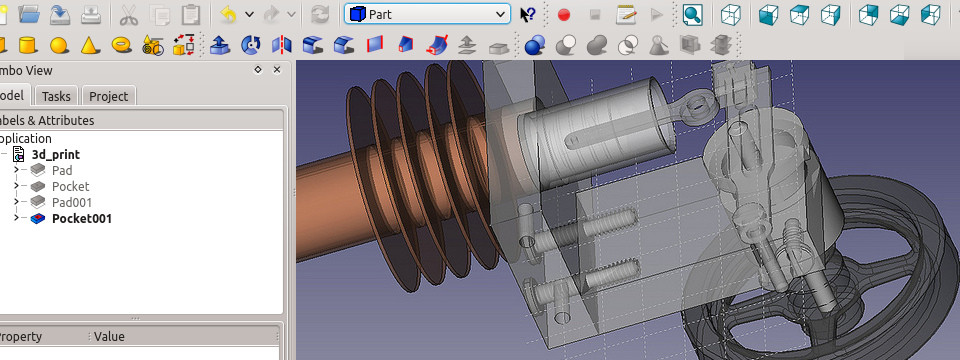
\includegraphics[width=14cm]{Img/CPD/freecad.jpg}
\centering
\caption{\textbf{\footnotesize{Freecad con un modelo mecánico y sus partes}}}
\end{figure}


En este trabajo se aborda el concepto de diseño computacional con la utilización de modelos 3D paramétricos. Es indispensable que los diseños se generen en función de sus parámetros y además expongan sus características de manera comprensible por todas las partes involucradas. \vskip
Por ejemplo: un diseñador industrial puede comprender naturalmente parámetros como arista, vértices o normales pero un artista puede comprender sobre dimensiones, colores o materiales. En este caso es recomendable que los modelos 3D en este caso se presenten en función de los parámetros conocidos por el artista.
Para ello surge la necesidad de una comunicación eficiente de los modelos 3D entre los interesados, y así gracias al diseño iterativo lograr la colaboración para generar nuevas soluciones.




\subsection{CAD Paramétrico especificado en algoritmos} 
El diseño paramétrico también es posible a través de las interfaces de secuencias de comandos del inglés \textit{scripting}\footnote{Un script es un programa informático usualmente simple, que por lo general se almacena en un archivo de texto plano. }. Las interfaces de scripting permiten a los diseñadores escribir código para automatizar partes del software. Los desarrolladores de software como AutoCAD\footnote{AutoCAD es un software de CAD utilizado para dibujo 2D y modelado 3D, Desarrollado y comercializado por la empresa Autodesk.}, incluso en 1982, se dieron cuenta de que la inclusión de estas interfaces les permitía ``Evitar muchas cosas personalizadas de codificación y aplicación que de lo contrario se les pediría". Diez años más tarde, en 1992, cuando Mark Burry\footnote{Mark Cameron Burry es un arquitecto neozelandés y profesor de Arquitectura del Royal Melbourne Institute of Technology en Melbourne.} quería modelar las hipérbolas paramétricamente para la Sagrada Familia, en lugar de pedirle a la empresa Autodesk que incluyera una función de hipérbola en AutoCAD, utilizó la interfaz de scripting para desarrollar una propia. El script de Burry tenía tres parámetros de entrada: un punto de origen, un punto mínimo y un punto de asíntota. Estos parámetros se alimentan a través de una serie de ecuaciones explícitas escritas en código AutoLISP\footnote{AutoLISP es un lenguaje de programación derivado del lenguaje Lisp. Es utilizado para generar rutinas en AutoCAD y sus derivados.} para emitir una hipérbola. 

El script, con sus parámetros de entrada, funciones explícitas y salidas es una realización arquetípica de la definición matemática de paramétrico. Ipek Dino ha argumentado que los scripts son inherentemente paramétricos, señalando que \textit{``los sistemas paramétricos se basan principalmente en principios algorítmicos ya que un algoritmo toma un valor o un conjunto de valores como entrada, ejecuta una serie de pasos computacionales que transforman la entrada y finalmente produce un valor o un conjunto de valores como salida".}
\vskip Por lo tanto, las interfaces de scripting accesibles en la mayoría de los paquetes de software están naturalmente predispuestas a crear modelos paramétricos. (\citeauthor{Dino2012}, \citeyear{Dino2012}) 

Estas interfaces se puede encontrar en programas como OpenSCAD\footnote{\url{http://www.openscad.org/}}, una aplicación FLOSS para crear objetos sólidos de CAD utilizando geometría constructiva de sólidos (CSG). No es un editor interactivo sino un compilador 3D basado en un lenguaje de descripción textual. Un documento de OpenSCAD especifica primitivas geométricas y define como son modificadas y manipuladas para reproducir un modelo 3D.



En la última década se ha visto la aparición de un nuevo tipo de interfaz de secuencias de comandos, la interfaz visual. La programación visual implica representar programas no como texto, sino como diagramas. Un ejemplo es Grasshopper \footnote{ \url{http://www.grasshopper3d.com/}} que se basa en gráficos que mapean el flujo de relaciones desde parámetros, a través de funciones definidas por el usuario, concluyendo normalmente con la generación de geometría. Los cambios en los parámetros o las relaciones del modelo hacen que los cambios se propaguen a través de las funciones explícitas para volver a dibujar automáticamente la geometría. Como tal, son otra forma de crear un modelo paramétrico.


\begin{figure}[h]
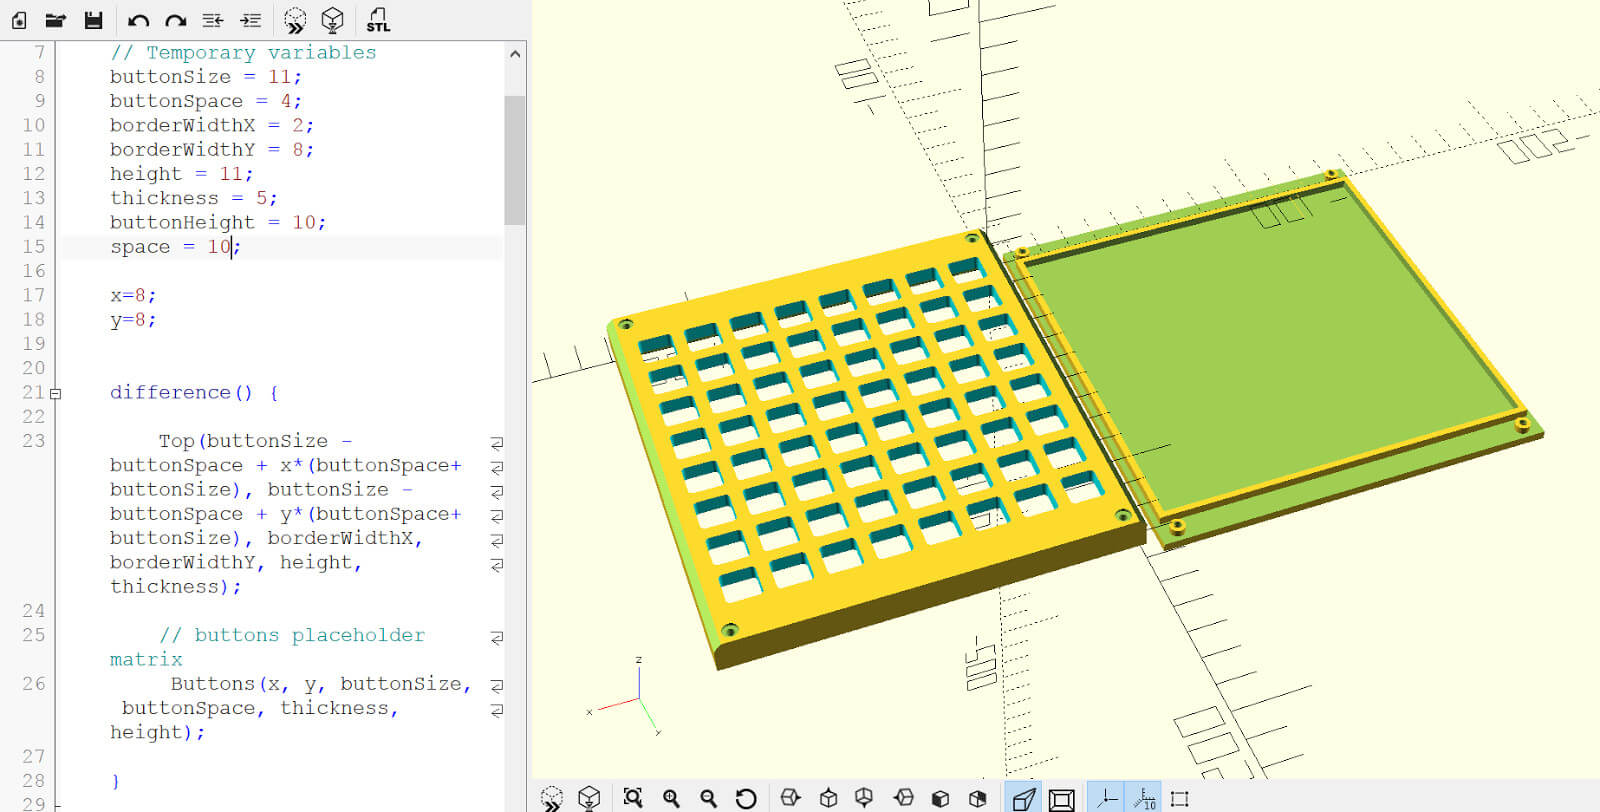
\includegraphics[width=14cm]{Img/CPD/openscadc.jpg}
\centering
\caption{\textbf{\footnotesize{Interfaz de OpenSCAD con el código que genera el modelo 3D}}}
\end{figure}

\begin{figure}[h]
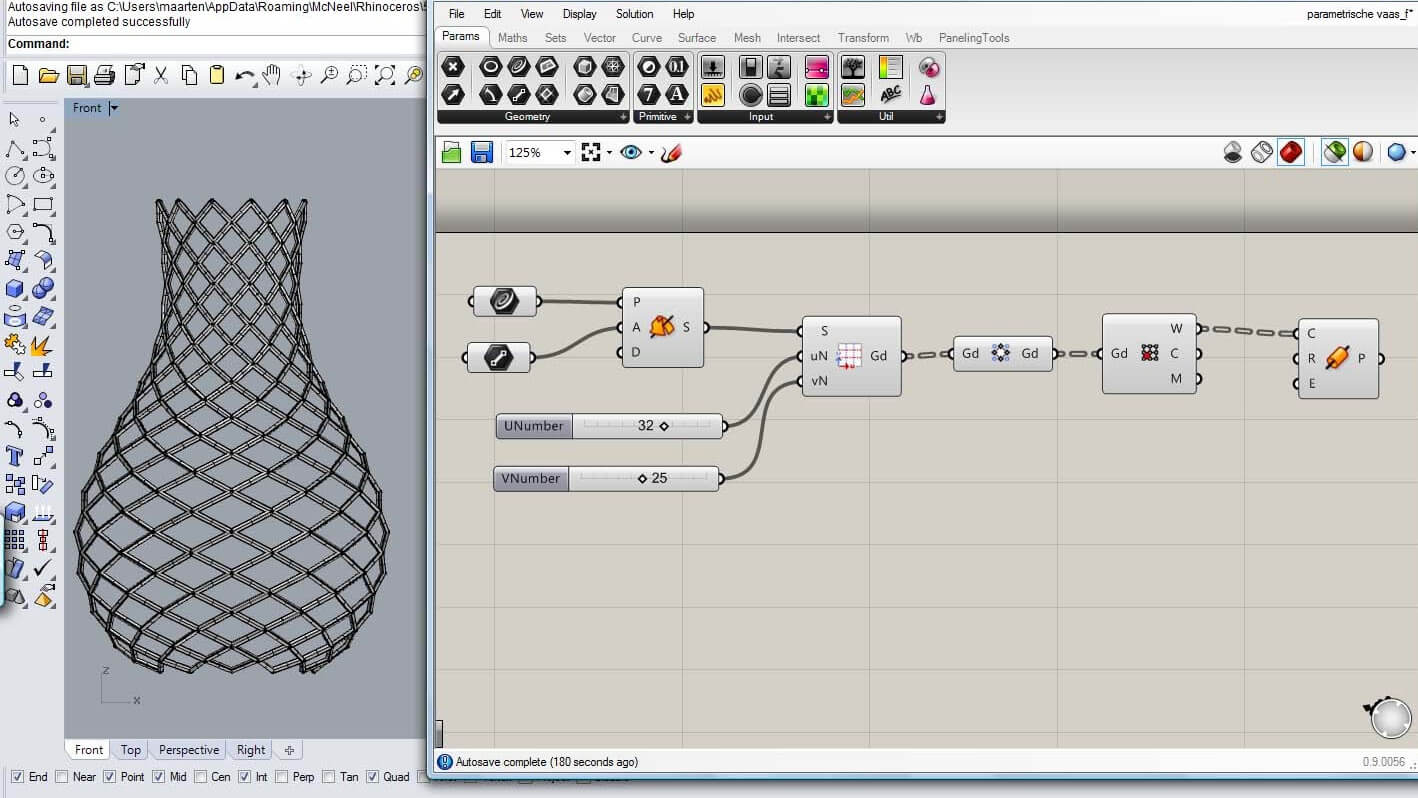
\includegraphics[width=14cm]{Img/CPD/rhinoc.jpg}
\centering
\caption{\textbf{\footnotesize{Rhinoceros con Graphopper, a la derecha se puede ver el diagrama que genera el modelo 3D}}}
\end{figure}


\clearpage
\subsection{CAD colaborativo y distribuido}
Para una efectiva colaboración no basta con una comunicación iterativa en la que se intercambian pocos datos del producto y siempre de arriba hacia abajo (“top-down”), sino que es necesario disponer de un repositorio\footnote{Un repositorio, depósito o archivo es un sitio centralizado donde se almacena y mantiene información digital, habitualmente bases de datos o archivos informáticos.} común de datos que vayan más allá de la geometría representada en planos, incluyendo documentos de especificaciones, instrucciones de montaje, etc. y todos ellos en cualquier formato digital: texto, CAD/CAM/CAE, PDM, audio, vídeo y combinaciones de ellos.
Saber trabajar en colaboración se convierte en un valor agregado, sobre todo si ésta es suministradora de componentes o sistemas para ser integrados en el producto final y para lograr esto es indispensable aprovechar el contexto actual de las nuevas tecnologías web y sus posibilidades. \citep{Ruiz}


En función de la naturaleza del diseño como trabajo colaborativo, el \textit{CAD distribuído} y el \textit{CAD integrado} se han convertido en un tema importante.\vskip
\textquote{\textit{El \textbf{CAD distribuído} implica que los datos CAD están disponibles a través de una red distribuída}}\citep{Synco1993}. El CAD integrado implica que los datos CAD se pueden leer por más
que un programa de computadora, por ejemplo, sistemas CAD de una variedad de empresas y otros tipos de programas de computadora, como herramientas de análisis.\vskip
Tanto el hardware como las tecnologías de software evolucionaron para admitir la comunicación y el acceso multiusuario a los datos de diseño, la forma de acceso varía desde archivos compartidos hasta accesos compartidos mediante Sistemas de Gestión de Bases de Datos en inglés \textit{Data Base Management System} (DBMS)\footnote{\url{https://en.wikipedia.org/wiki/Database}}. El modelado de los datos de diseño proporciona la base para establecer el semántica de los datos compartidos. Se supone que en \textit{el CAD distribuido permite el acceso a los datos de diseño a través de un sistema de CAD predeterminado o bien un DBMS}.\vskip
Los esfuerzos hacia la integración del CAD generaron como resultado el desarrollo de varios formatos  estándares para el intercambio de datos en ingles \textit{Data Exchange}, así como muchos "no estándares". Los formatos estándares de intercambio han variado desde formatos para datos de dibujo técnico hasta formatos para modelos de productos. 
DXF\footnote{\url{https://es.wikipedia.org/wiki/DXF}} e IGES\footnote{ \url{https://es.wikipedia.org/wiki/IGES}} son algunos formatos que resultaron de los esfuerzos en el intercambio de bases de datos de gráficos entre sistemas CAD.\vskip

La falta de características de diseño en los estándares de intercambio de datos, como topología, relación entre objetos, etc., obligó un cambio en el enfoque hacia los estándares de \textit{intercambio de datos de productos}. El enfoque en el modelado de productos (por ejemplo, PDES- STEP\footnote{\url{https://pdesinc.org/}}, etc.) han puesto énfasis en el modelado sólido 3D, en la geometría, las características esenciales de los modelos, los datos no geométricos y el modelando del producto como un conjunto de conceptos u objetos.

\subsubsection{Identificación de sistemas CAD según su uso}
Los sistemas CAD distribuidos y colaborativos se pueden identificar en una matriz distinguiendo entre tiempo y espacio, como se puede ver en la Figura \ref{fig:tablacad}:

\begin{enumerate}
\item El uso de CAD en el mismo lugar al mismo tiempo es posible con un Interfaz CAD de usuario único, donde uno o más los diseñadores pueden sentarse en una estación de trabajo para diseñar los modelos.
\item El uso de CAD en el mismo sitio pero en tiempos diferentes es posible gracias a la gestión de datos técnicos donde los datos están disponibles para la misma persona u otros miembros del equipo de diseño después que una sesión de diseño CAD se completa.
\item El uso de CAD al mismo tiempo en sitios diferentes se denomina como
\textit{CAD colaborativo o bien Co-Diseño CAD}. En esta situación, diferentes diseñadores pueden ver y modificar el diseño en diferentes ubicaciones, viendo la misma imagen en la pantalla y comunicándose entre sí.
\item El uso de CAD en sitios diferentes en tiempos diferentes es posible gracias a la distribución de datos CAD a través de una red (CAD distribuido), permitiendo a los diseñadores acceder a los datos independientemente de su ubicación y disponibilidad.
\end{enumerate}


\begin{figure}[h]
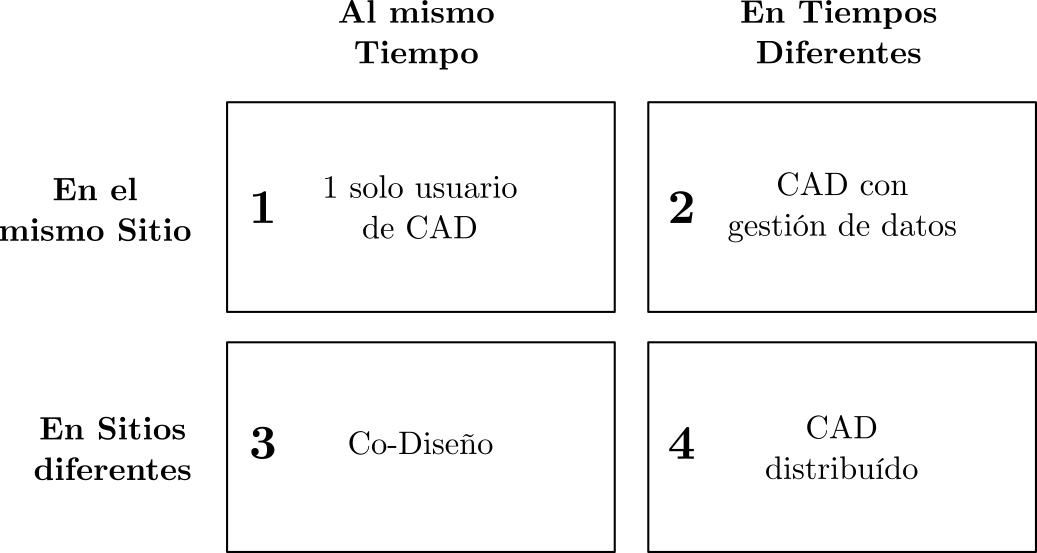
\includegraphics[width=10cm]{Img/CPD/cad-time.png}
\centering
\caption{\textbf{\footnotesize{El uso del CAD en el espacio y tiempo}}}
\label{fig:tablacad}
\end{figure}


\subsubsection{ Esquema distribuido para la colaboración }

La \textit{colaboración sincrónica} indica que la colaboración se produce cuando todos los miembros del equipo de diseño trabajan en los mismos documentos, información o problema al mismo tiempo. La naturaleza amplia de la colaboración en el diseño implica que el soporte informático para dicha actividad debe proporcionar flexibilidad en la comunicación de datos e ideas de diseño. \vskip
El diseño colaborativo involucra muchos tipos de conocimiento de diferentes dominios.
Los diseñadores requieren diferentes vistas del diseño y tienen intereses sustancialmente diferentes con respecto al desarrollo de la solución de diseño y su representación asociada. Se necesitan múltiples niveles de abstracción para tratar con la diversidad del conocimiento. En términos de soporte informático, se necesitan diferentes formas de interactuar con otros diseñadores y herramientas para respaldar la diversidad del diseño.\vskip

El desarrollo del soporte informático para la colaboración sincrónica se puede lograr mediante un espacio de trabajo compartido, como se ilustra en la Figura \ref{fig:espacio0}. El espacio de trabajo compartido es el medio a través del cual se produce la comunicación entre los participantes en el diseño colaborativo. Un espacio de trabajo compartido no solo proporciona una comunicación visual flexible y efectiva, sino que también proporciona un medio en el que un diseñador puede comprender el modelo/diseño de otro participante sin necesidad de tener el mismo vocabulario. Por lo tanto, también es importante compartir la representación subyacente de los elementos de diseño en el espacio de trabajo.

\begin{figure}[h]
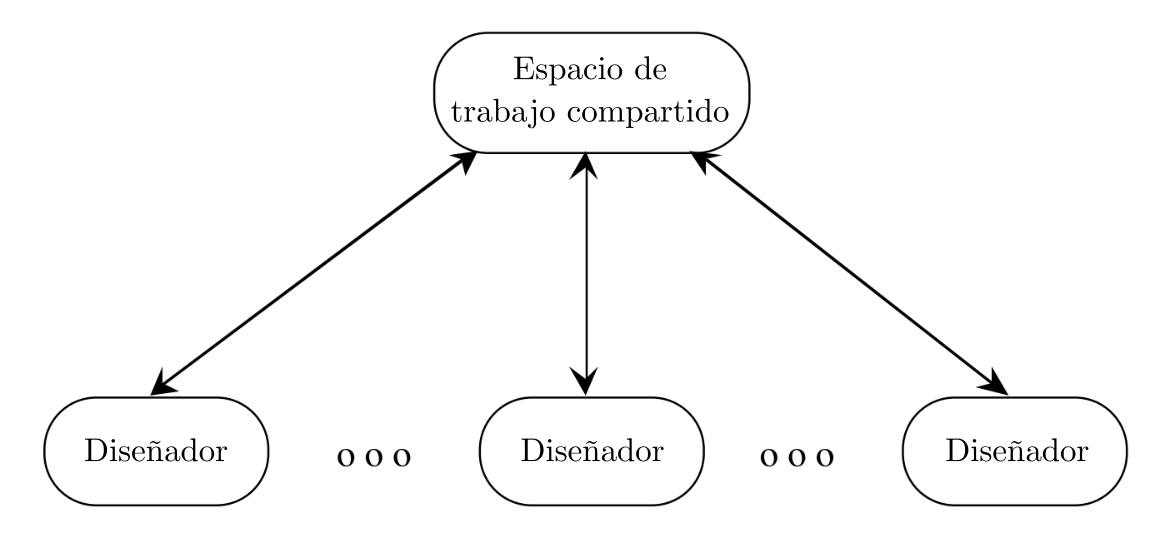
\includegraphics[width=12cm]{Img/CPD/cad-shared0.png}
\centering
\caption{\textbf{\footnotesize{Espacio de trabajo compartido}}}
\label{fig:espacio0}
\end{figure}

Esto implica que el modelo ilustrado en la Figura \ref{fig:espacio0} es demasiado simplista. Un espacio de trabajo compartido CAD tiene dos significados:
\begin{enumerate}
\item El espacio de trabajo con el que los diseñadores humanos ven e interactúan, y
\item La representación compartida del problema de diseño que utiliza la propia computadora para la persistencia y la comunicación entre procesos.
\end{enumerate}

Se consideran dos categorías de espacio de trabajo:

\begin{enumerate}
    \item Representación visual compartida y
    \item Representación subyacente compartida.
\end{enumerate}
La necesidad de mantener dos formas de representación compartida proviene de los requisitos de un sistema multiusuario en el que los participantes puedan ver el trabajo de los demás, proporcionado por la representación visual compartida (modelo 3D), con la posibilidad de que el sistema mantenga una o más representaciones de la solución de diseño (versiones) y cualquier conocimiento de dominio relevante proporcionado por la representación subyacente (archivos extra). Los cuatro componentes nesesarios para cumplir esto son:

\begin{enumerate}
    \item \textit{Servidor de sesión}. Inicia el proceso de solicitud que se encarga de configurar la sesión para el diseño colaborativo.
    \item \textit{Coordinador}. Un proceso de aplicación especial que incorpora la gestión y el control de datos entre la aplicación y el espacio de trabajo.
    \item \textit{Representación visual compartida}. Intercambio visual de elementos de diseño desde el punto de vista geométrico.
    \item \textit{Representación subyacente}. Conjunto genérico de objetos asociados a los modelos y los procesos.
\end{enumerate}

\begin{figure}[h]
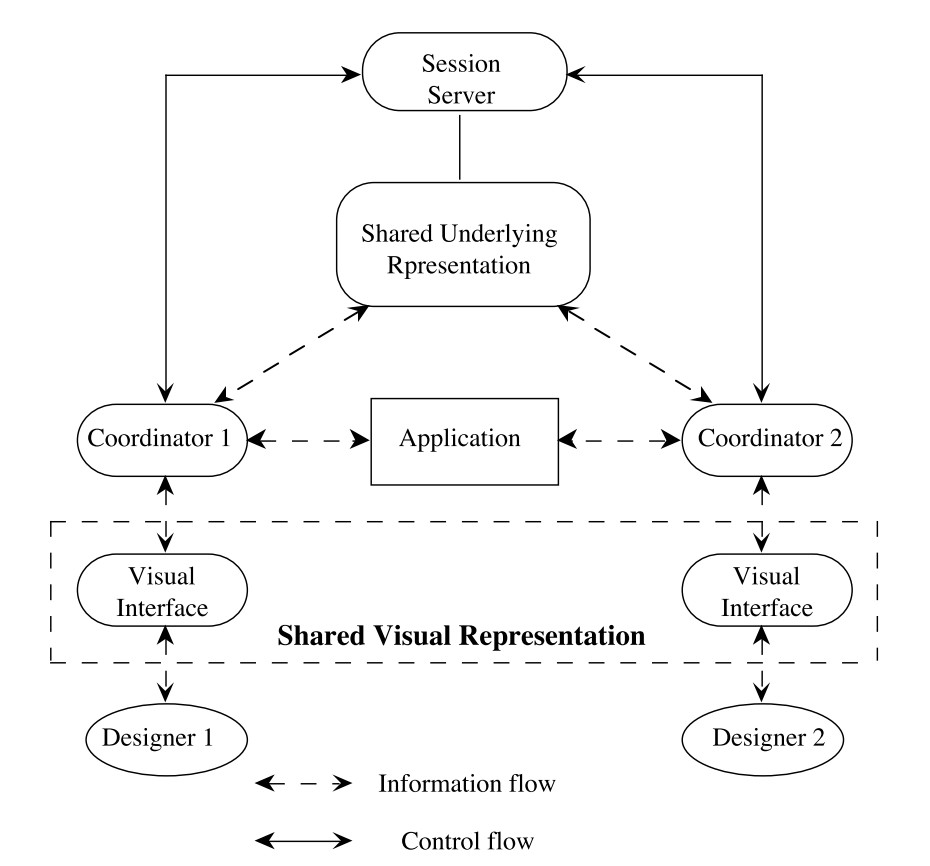
\includegraphics[width=14cm]{Img/CPD/cad-shared1.jpg}
\centering
\caption{\textbf{\footnotesize{Modelo de sistema CAD colaborativo}}}
\label{fig:sistemaco}
\end{figure}



Las herramientas de diseño CAD tradicionales fueron pensadas para un usuario, por ende tienen limitaciones para soportar el entorno de desarrollo colaborativo de productos CPD y de forma rápida como requiere el mercado. En un proceso de desarrollo distribuido, se necesita una comunicación efectiva y de alta velocidad porque la mayoría de los errores de diseño se deben a la falta de comunicación entre los equipos de diseño distribuidos.\vskip
Los sistemas de información distribuída que se han aplicado para CPD se pueden clasificar en 3: 
\begin{itemize}
    \item \textit{Web services}
    \item \textit{Remote services}
    \item \textit{Remote repositories}
\end{itemize}
Los sistemas basados en \textbf{web services} tienen ventajas sobre los otros dos porque son relativamente sencillos de diseñar e implementar, reducen los problemas de la instalación de software y facilitan la participación. \citep{Nyamsuren2015}

\clearpage
\section{Informática Gráfica: perspectiva del trabajo}

No cabe duda de que la vista es una de las principales vías de entrada de información al cerebro. La interpretación por éste de la \textbf{información visual}, sólo es posible después de un proceso de aprendizaje; una vez que se aprenda a tratar la información visual, como por ejemplo, reconocer los objetos y la utilidad de cada uno, dicha información ayuda a la toma decisiones. \vskip
A pesar de la disparidad que puede haber entre los diferentes medios de registro, por ejemplo, entre una hoja de papel y una pantalla de computadora, el conocimiento básico necesario para registrar información visual es el mismo.
Así, en el papel se necesitan conocer los puntos a entintar y su color, y en la pantalla es necesario saber qué píxeles de la pantalla se deben activar para que emitan luz del color apropiado. \vskip
Haciendo un poco de abstracción, si se llaman \textit{“puntos del espacio de referencia”}
a los puntos del papel, de la pantalla, o de cualquier otro medio de registro, \textit{la información necesaria para asignar características o propiedades ópticas a cada punto del espacio de referencia, tales como color, opacidad, etc., es o se conoce como \textbf{información gráfica}}.\vskip

Tomando como referencia la definición anterior, podemos definir la \textbf{Informática Gráfica} (IG), como \textit{el área de la Informática que se dedica al estudio y desarrollo de procesos que permitan el tratamiento automático de la información gráfica}.\vskip 
La información gráfica con que trabaja la IG puede estar dada por conjuntos de infinitos puntos, definidos en espacios continuos, o bien por conjuntos finitos definidos sobre espacios discretos, es decir, direccionables exclusivamente mediante números enteros. En el diagrama de la Figura \ref{fig:grafica0} podemos ver los cuatro tipos de información gráfica en los espacios 2 y 3D.

\begin{figure}[h]
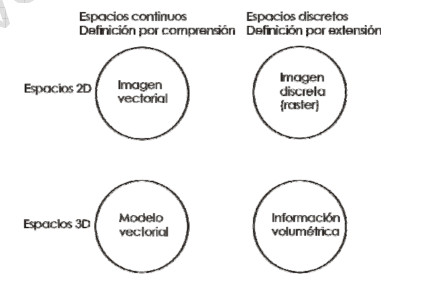
\includegraphics[width=14cm]{Img/CPD/grafica0.jpg}
\centering
\caption{\textbf{\footnotesize{Modelo de sistema CAD colaborativo}}}
\label{fig:grafica0}
\end{figure}

En los espacios continuos, la información gráfica definida en un espacio 2D se conoce como \textbf{imagen vectorial}, y si el espacio es 3D, entonces se llama \textbf{modelo vectorial}. Algo similar ocurre en los espacios discretos. Así, en 2D la información gráfica recibe el nombre de \textbf{imagen raster}\footnote{Una imagen ráster o mapa de bits es un archivo que representa una matriz de píxeles o puntos de color, a partir de un modelo vectorial 3D} o imagen discreta; en cambio, en los espacios discretos 3D es conocida como \textbf{información volumétrica}.

En la actualidad, la mayoría de las aplicaciones gráficas o \textit{sistemas gráficos} se limitan al tratamiento de la información gráfica definida en espacios de 2 y 3 dimensiones, aunque hay sistemas que permiten el estudio, tratamiento y visualización de información gráfica en espacios de dimensión mayor, espacialmente en 4D. Este trabajo se limita a estudiar la IG con información definida en 2 y 3D exclusivamente.

\subsection{Campos que abarca la Informática Gráfica}
Hay muchas formas de tratar información gráfica, y cada una de ellas puede dar lugar a un campo o subárea de especialización dentro de la IG.
Cualquiera de los cuatro tipos de información gráfica que se muestra en la Figura \ref{fig:grafica0} puede ser la fuente de información con la que puede trabajar un proceso gráfico. Igualmente, generar información de uno de los cuatro tipos suele ser el principal objetivo de dichos procesos aunque, en algunas ocasiones, lo que se pretende es obtener información numérica (cálculo de superficies, volúmenes, estadísticas, etc.).
Según esto, se puede pensar en clasificar los diferentes campos y procesos de la IG, en función del tipo de información de entrada y salida, y de la clase de proceso que se efectúe con la información gráfica.
Entonces, si relacionamos mediante una flecha la clase de información de entrada que requiere un proceso o sistema gráfico, con el tipo de información de salida generada por éste, a partir del diagrama de la Figura \ref{fig:grafica0} e incorporando la información numérica, se puede construir un diagrama, tal como se muestra en la Figura \ref{fig:grafica1}, donde quedan especificados los principales campos de la IG.

\begin{figure}[h]
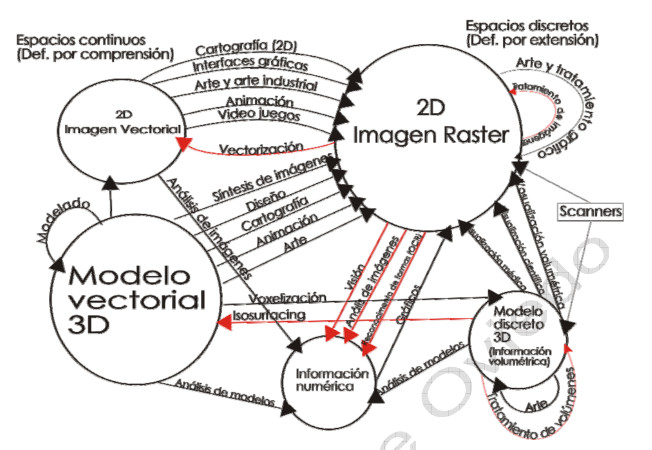
\includegraphics[width=10cm]{Img/CPD/grafica1.jpg}
\centering
\caption{\textbf{\footnotesize{Campos más significativos de actuación de la Informática Gráfica}}}
\label{fig:grafica1}
\end{figure}

En el diagrama anterior aparecen los principales campos que abarca la IG, así como algunos de los procesos más comunes, como son los de conversión de unos tipos de información a otros. Además, es importante señalar que las flechas del diagrama indican el objetivo final del campo de estudio o del proceso, y no necesariamente el camino seguido para alcanzar dicho objetivo. Por ejemplo, en la Síntesis de Imágenes, uno de los métodos para conseguir una imagen raster a partir del modelo vectorial 3D, genera una imagen vectorial como paso previo a la obtención de la imagen raster.

A continuación definimos los dos campos de la IG que son objetos de estudio en el trabajo de investigación: La \textit{Síntesis de Imágen} y el \textit{Modelado}. En la Figura \ref{fig:grafica2} queda definido el diagrama de estudio.



\begin{figure}[h]
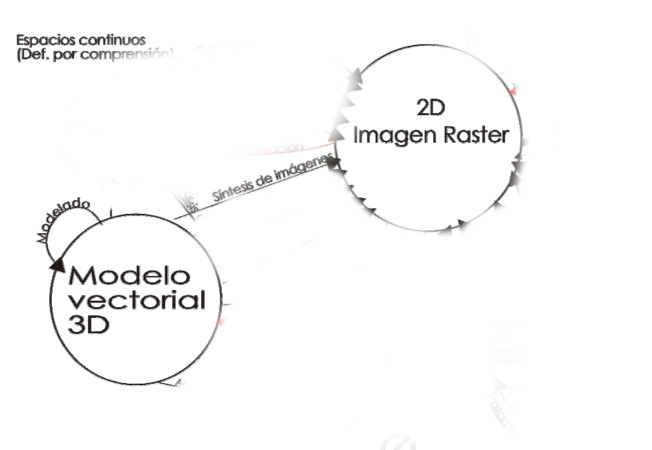
\includegraphics[width=14cm]{Img/CPD/grafica2.jpg}
\centering
\caption{\textbf{\footnotesize{Campos de la Informática Gráfica definidos para el estudio}}}
\label{fig:grafica2}
\end{figure}


\subsection{Síntesis de Imágenes}

Un elemento indispensable para poder visualizar modelos 3D en una pantalla es la \textit{Síntesis de imágenes}, definida como un \textit{campo de la informática gráfica que se dedica principalmente al estudio y desarrollo de procesos para sintetizar imágenes raster}.\vskip
En la mayoría de los casos su principal objetivo es obtener imágenes de calidad, no importando demasiado si el modelo vectorial de partida es consistente (coherente) o no. Sin embargo, en el diseño CAD es fundamental que los modelos estén bien definidos (consistentes). La visualización en estos contextos es auxiliar (aunque necesaria), por lo que no tiene demasiada importancia la calidad de las imágenes, al menos en las primeras fases de diseño.\vskip

El conjunto de procesos que directa o indirectamente permiten la síntesis de imágenes debería conocerse como sintetizador de imágenes, o algo parecido. Sin embargo, se utiliza un término más ambiguo, como el de ``sistema gráfico” (SG). 
La visualización o ``rendering" se produce en función de las condiciones establecidas por el observador, cámara o visor. Es necesaria la presencia de una cámara, ya que el propósito de un sistema gráfico es crear una imagen bidimensional a partir de un modelo tridimensional, lo que implica la imposibilidad de mostrar simultáneamente en pantalla toda la información del modelo.
Esquemáticamente, el objetivo principal de un sistema gráfico se resume en la Figura \ref{fig:grafica3}.

\begin{figure}[h]
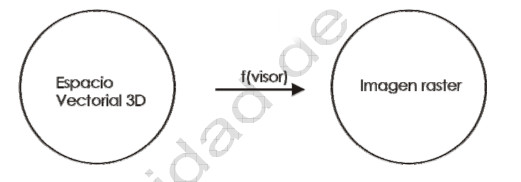
\includegraphics[width=8cm]{Img/CPD/grafica3.jpg}
\centering
\caption{\textbf{\footnotesize{Rasterización de una imagen}}}
\label{fig:grafica3}
\end{figure}

\subsubsection{Estructuración de la Síntesis de Imágenes}
Como toda disciplina la Síntesis de Imágenes se organiza y subdivide en campos de trabajo, principalmente para evitar la mezcla de conceptos, y facilitar así su estudio. Para ello, se busca y aplicar uno o más criterios de organización que permitan la estructuración coherente del área. Son dos los criterios principales que se utilizan: \textit{el método de síntesis de imágenes utilizado, y el modelo de iluminación que se aplica}.

\begin{description}

\item \textbf{a) Métodos de síntesis de las imágenes} \vskip
El criterio principal que se utiliza en la estructuración de la Síntesis de Imágenes es \textit{el camino que se sigue (método) para sintetizar las imágenes raster}.

\begin{enumerate}
    \item \textbf{Síntesis estándar} \vskip
    Como se indica en la Figura \ref{fig:grafica4}, la información se busca en el espacio vectorial, según las condiciones del visor, formando (mediante proyecciones) una imagen vectorial. Si se dispusiese de un monitor vectorial, la imagen creada podría ser mostrada directamente en dicho monitor. Sin embargo, hoy en día la mayor parte de los monitores son de tipo raster, lo que significa que la imagen vectorial se debe rasterizar, para que pueda ser mostrada en esta clase de monitores.
    
    \begin{figure}[h]
    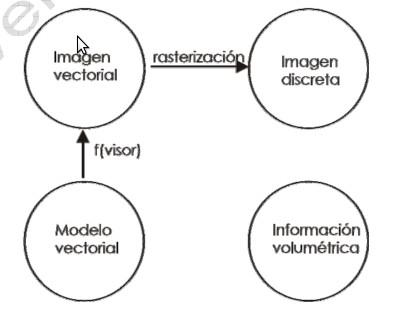
\includegraphics[width=6cm]{Img/CPD/grafica4.jpg}
    \centering
    \caption{\textbf{\footnotesize{método de síntesis estándar}}}
    \label{fig:grafica4}
    \end{figure}

    \item \textbf{Síntesis directa} \vskip
    La imagen raster se forma buscando la información gráfica directamente del espacio vectorial. Para ello, se utilizan una serie de procesos que emulan el movimiento y características de la luz natural. La Figura \ref{fig:grafica5} muestra un esquema de este camino de síntesis, al cual se le denomina método directo de síntesis, o simplemente síntesis directa
    
    \begin{figure}[h]
    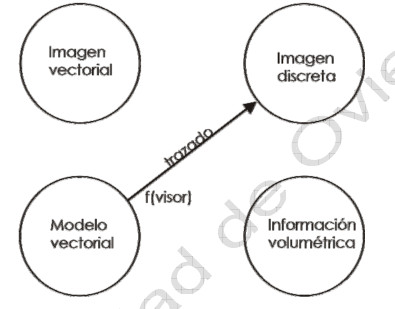
\includegraphics[width=6cm]{Img/CPD/grafica5.jpg}
    \centering
    \caption{\textbf{\footnotesize{método de síntesis directa}}}
    \label{fig:grafica5}
    \end{figure}
    
     \item La tercera y última ruta mostrada en la Figura \ref{fig:grafica6}, aunque se emplea con frecuencia en la visualización volumétrica, no se utiliza en la Síntesis de imágenes, ya que no se consigue mayor calidad en las imágenes, pudiendo incluso disminuir en muchos casos. En cambio, el camino inverso sí es frecuentado, pues la conversión de la información volumétrica en vectorial (isosurfacing) permite la visualización por cualquiera de los métodos anteriores.
    
    \begin{figure}[h]
    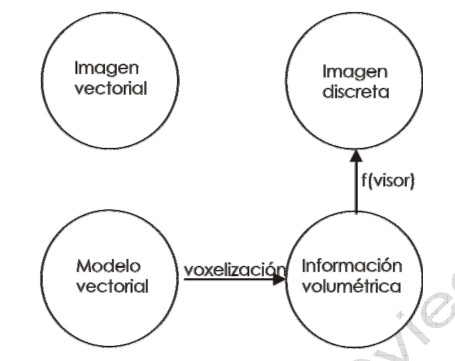
\includegraphics[width=6cm]{Img/CPD/grafica6.jpg}
    \centering
    \caption{\textbf{\footnotesize{Renderizado directo de volúmenes (DVR)}}}
    \label{fig:grafica6}
    \end{figure}
    
    \end{enumerate}



\item \textbf{b) Modelos de Iluminación} \vskip
El objetivo final de los modelos de iluminación es \textit{determinar la cantidad (intensidad) y el color de la luz que llega a un punto dado en la superficie de los objetos. Para ello, modelan una serie de efectos lumínicos, como la transparencia, reflexiones de la luz, textura de las superficies y sombras}. Estos efectos luminosos dependen del número, tamaño y posición de las fuentes de luz, por lo cual los modelos de iluminación han de tener en cuenta dichas fuentes.

\begin{enumerate}
    \item \textbf{Modelos Locales}\vskip
    En el cálculo de la iluminación de un punto dado no se tiene en consideración la luz emitida (reflejada o transmitida) por los objetos circundantes.
    \item \textbf{Modelos Globales}\vskip
    En el cálculo de la iluminación se tiene en cuenta parte de la luz aportada por los objetos vecinos.
    \item \textbf{Modelos SemiGlobales}\vskip
    El modelo tiene en consideración \textbf{toda} la luz aportada por los objetos circundantes.
\end{enumerate}

Lo que diferencia a un modelo global de uno semiglobal es si el modelo realiza o no cálculos ajustados sobre la iluminación debida a la luz difusa, ya que ésta es una de las cuestiones más difíciles de evaluar. Por lo tanto, es posible considerar los modelos globales como una extensión de los semiglobales, incorporando el cálculo de la aportación difusa.
Como era de esperar, los modelos de iluminación computacionalmente más económicos y sencillos son los modelos locales, y los más caros y complejos los globales. Sin embargo, la complejidad y el tiempo de cálculo extra en los modelos semiglobales y globales quedan compensados con una mayor calidad de las imágenes sintetizadas.

\item \textbf{c) Compatibilidad entre los métodos de síntesis y los modelos de iluminación} \vskip
Para un método de síntesis dado, algunos modelos de iluminación son más fáciles de implantar que otros, dependiendo de la naturaleza del método y de la complejidad del modelo de iluminación.\vskip
Así, los modelos locales pueden ser aplicados sin dificultad tanto en la síntesis estándar, como en la directa. En cambio, los modelos semiglobales son más fáciles de implantar en la síntesis directa, aunque también es posible utilizarlos en la síntesis estándar, si bien, al precio de un aumento considerable en la complejidad de los algoritmos.\vskip
Por otro lado, es más fácil utilizar los resultados de los cálculos sobre la luz difusa en la síntesis estándar que en la directa. Esto lleva a la necesidad de los planteamientos de síntesis híbridos, para incorporar en los modelos semiglobales (síntesis directa) los resultados de los cálculos sobre la aportación difusa (síntesis estándar).

\item \textbf{d) Procesos de visualización}\vskip

A la utilización conjunta de un método de síntesis y de un modelo de iluminación (que obviamente han de ser compatibles entre sí), se suele llamar \textbf{proceso de visualización}.\vskip
Cada proceso de visualización constituye un área de especialización dentro de la Síntesis de Imágenes, debido principalmente a las diferencias existentes entre las técnicas utilizadas en los métodos de síntesis estándar y el directo.
Teniendo en cuenta los métodos de síntesis, los modelos de iluminación y las compatibilidades entre ellos, en la tabla 2 queda establecida la estructuración actual de la Síntesis de Imágenes. 

En ella aparecen los diferentes procesos de visualización (campos) de la Síntesis de Imágenes:

\vskip

\begin{enumerate}
    \item \textbf{Rendering estándar}\vskip
    Es el proceso de visualización más difundido, ya que no requiere equipos demasiado potentes para conseguir, en un tiempo razonable, imágenes de calidad aceptable. Cuando el proceso incorpora técnicas de los modelos de iluminación semiglobales, usualmente se continua utilizando el mismo término, o bien simplemente se le añade el calificativo de “mejorado” (enhanced).
    
    \item \textbf{Ray Tracing}\vskip
    El algoritmo trazador de rayos en inglés ray tracing, inicialmente era desechado debido al gran potencial de cálculo que requiere, lo que implicaba una gran lentitud en la generación de las imágenes. Sin embargo, a medida que iba aumentando la velocidad de las computadoras y mejorando las técnicas de aceleración del algoritmo ray tracing fue ganando adeptos, debido sobre todo a la gran calidad de las imágenes que genera. Hoy día, no existe prácticamente ningún sistema gráfico que no ofrezca la posibilidad de generar imágenes mediante este algoritmo. El algoritmo trazador de rayos es más rápido y fácil de implantar si se aplica un modelo local \textbf{ray casting} aunque, claro está, la calidad de las imágenes obtenidas es inferior.
    
    \item \textbf{Radiosity}\vskip
    Basándose en técnicas utilizas en la calorimetría, hacia finales de 1980 fueron desarrollados procesos para el cálculo de la aportación luminosa debida a la luz difusa. Con ello aparecieron los modelos globales y un nuevo campo de la Síntesis de Imágenes, conocido como algoritmo de radiosidad o radiosity. Este algoritmo es uno de los más utilizados en la gráfica de alto \textcolor{red}{standing} debido a la gran calidad de las imágenes que sintetiza. 
    
    \begin{figure}[h]
    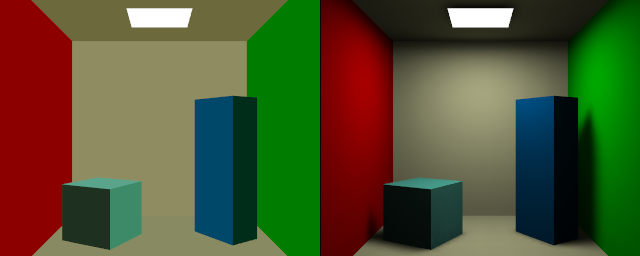
\includegraphics[width=12cm]{Img/CPD/grafica7.png}
    \centering
    \caption{\textbf{\footnotesize{Comparación de ray tracing con ray tracing + radiosity}}}
    \label{fig:grafica7}
    \end{figure}
    
\end{enumerate}

ACA VA LA TABLA

\item \textbf{e) Características comunes en los procesos de visualización}\vskip

Aunque las técnicas utilizadas en los procesos de visualización difieren de unos a otros, la filosofía en todos ellos es básicamente la misma. Son tres los objetivos principales de cualquier visualizador. 

\begin{itemize}
    \item Dependiendo de la posición del observador en el espacio vectorial 3D, se han de localizar los puntos que caen dentro de su campo de visión, buscando sus propiedades físicas.
    \item A continuación, ha de calcular de forma individual o colectiva la iluminación que llega a cada uno de ellos, dependiendo del método utilizado.
    \item Por último, se ha de generar la imagen raster, discretizando la información que se tiene sobre los puntos visibles del espacio vectorial y sobre la luz que reciben

\end{itemize}

\end{description}


\subsection{Ray Tracing}

\subsubsection{Conceptos generales}
\label{section:ray-concept}

\textit{Todos los rayos de luz que atraviesen la pantalla han de converger en el punto de visión (ojo)}, esto es conocido como \textbf{modelo de ventana}. 
Si se traza un rayo desde el punto de visión a cada píxel de la pantalla, y se prolongan dichos rayos hasta que intersequen con los objetos que se encuentren en su camino, entonces es posible averiguar con qué objetos intersecan y el color de las superficies donde intersecan. Si se pinta los píxeles correspondiente con el color de los puntos de intersección, se obtiene la imagen del objeto que se trata de visualizar como en la Figura \ref{fig:ojo}. Los objetos visualizados son aquellos que se encuentran dentro del volumen de la pirámide, cuyas aristas pasan por los vértices de la ventana, y convergen en el punto de visión. En definitiva, el principio en el que se basa el algoritmo de ray tracing es el de trazar una línea entre el punto de visión y el espacio de objetos (modelos), a través de cada píxel de la pantalla. \vskip
En el modelo de ventana, si un fotón llega al ojo del observador, necesariamente ha tenido que cruzar la pantalla siguiendo la dirección del rayo.
Entonces, si se trazan exclusivamente los rayos de luz que parten del punto de visión, a través de los píxeles de la pantalla hacia el espacio vectorial (conocidos como rayos primarios), se asegura que el sistema gráfico trabaje únicamente con los rayos útiles. Cuando el trazado de rayos se realiza de esta forma, es conocido como \textbf{trazado hacia atrás}. 
Dado el ahorro de cálculos que implica el invertir el recorrido de los fotones, el trazado de rayos hacia atrás es el procedimiento utilizado. Por tanto, siempre que se trate de ray casting o ray tracing, ambos algoritmos efectúan el trazado hacia atrás. 


 \begin{figure}[h]
    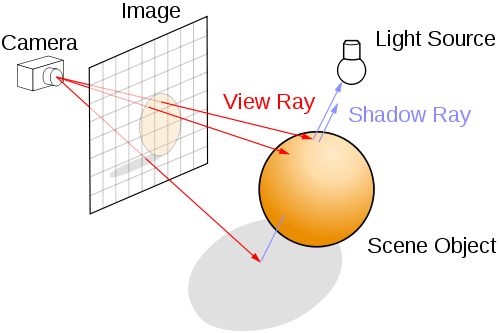
\includegraphics[width=12cm]{Img/GEO/geo-ojo1.png}
    \centering
    \caption{\textbf{\footnotesize{trazado de los píxeles }}}
    \label{fig:ojo}
    \end{figure}
    
Cualquiera que sea el método de visualización aplicado, el paso previo a la obtención de las imágenes es siempre el de colocar convenientemente los elementos del escenario (objetos, visor y fuentes) en un espacio de referencia
común, al que se llama \textbf{Sistema Universal de Referencia} \textbf{(SUR)}. Excepto las fuentes puntuales, normalmente los demás elementos del escenario poseen su propio sistema de referencia, siendo el \textbf{SRV} el \textbf{Sistema de Referencia del Visor}, y el \textbf{SRO} el \textbf{Sistema de Referencia de los Objetos}.
A menudo, las características del sistema de referencia general (SUR) y de los sistemas locales coinciden, aunque también es frecuente que la orientación del SRV sea opuesta a la del SUR. Por ejemplo, en la Figura \ref{fig:grafica8} vemos un SUR con orientación hacia la izquierda1, y un SRV con orientación hacia la derecha.

 \begin{figure}[h]
    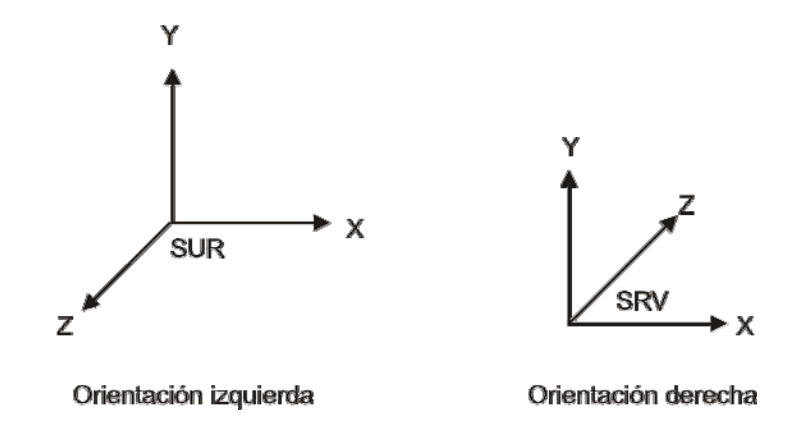
\includegraphics[width=8cm]{Img/CPD/grafica8.jpg}
    \centering
    \caption{\textbf{\footnotesize{ sistemas de referencia ortogonales con orientación opuesta }}}
    \label{fig:grafica8}
    \end{figure}
    

    
\subsubsection{Explicación del algoritmo}

Los modelos de iluminación semiglobales, además de considerar la contribución de las fuentes de luz, también tienen en cuenta la luz reflejada y la transmitida procedente de los objetos circundantes. El algoritmo trazador de rayos (ray tracing), que es una generalización del algoritmo de ray casting, utiliza un modelo de iluminación semiglobal.
Así, en la versión típica del algoritmo de ray tracing, el color (intensidad) en un punto de intersección rayo-superficie cualquiera viene determinado por tres tipos de aportaciones lumínicas:
\begin{itemize}
    \item Por un lado está la contribución o color local, que se debe a la iluminacióndirecta de las fuentes, y la luz ambiental. En definitiva, se trata de aplicar el modelo de iluminación local utilizado en ray casting.
    \item Por otro lado está la contribución o color reflejado, que consiste en la luz que llega al punto de intersección desde los objetos circundantes, siguiendo la trayectoria de reflexión de la luz.
    \item Por último, el algoritmo de ray tracing también cuenta con la aportación del color transmitido, que se debe la luz que llega al punto de intersección después de cruzar (traspasar) los objetos vecinos (si es que son transmisores de la luz), siguiendo la trayectoria de transmisión. 

\end{itemize}

En la Figura \ref{fig:grafica9} se pueden apreciar las tres contribuciones en un punto de intersección rayo-superficie dado.

\begin{figure}[h]
    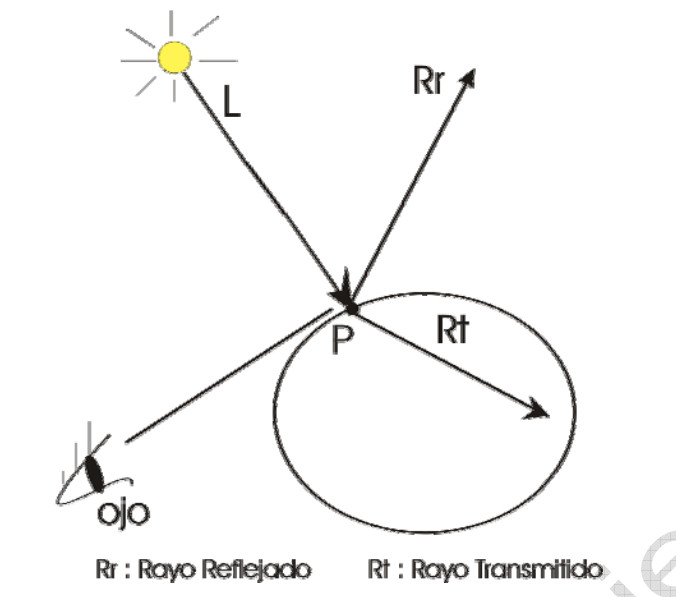
\includegraphics[width=8cm]{Img/CPD/grafica9.jpg}
    \centering
    \caption{\textbf{\footnotesize{ modelo de iluminación semiglobal utilizado con el algoritmo de ray tracing  }}}
    \label{fig:grafica9}
\end{figure}


\textbf{Definición del rayo: ecuación explícita o paramétrica}\vskip
Los parámetros que definen el rayo (recta) son los siguientes: 
$$R_0 = [X_0 , Y_0 , Z_0] \ \ punto \ de \ origen\ del \ rayo$$
$$R_d = [X_d , Y_d , Z_d] \ \ vector \ de \ dirección\ del \ rayo$$

Partiendo de las expresiones anteriores, se pueden expresar las coordenadas de cualquier punto $[x, y, z]$ de la recta R (rayo), en función de ``t”, como sigue: 

$$
   X_0 = X_0 + X_d.t
$$
$$
   Y_0 = Y_0 + Y_d.t
$$
\begin{equation}
   Z_0 = Z_0 + Z_d.t
\end{equation}

Dando distintos valores a ``t”, se obtienen todos los puntos de la recta. Escribiendo en formato vectorial las expresiones anteriores, se obtiene la \textbf{ecuación explícita del rayo (recta)}, es decir: 
\begin{equation}
R(t) = R_0 + R_d.t \ \ siendo \ t>0 \ para \ el \ rayo
\label{eq:rayos}
\end{equation}

Es conveniente que el vector de dirección del rayo esté normalizado, es decir, que su módulo sea unitario ${x_d}^2 + {y_d}^2 + {z_d}^2 = 1$. De esta forma``t” representa la distancia desde el origen del rayo, referida al sistema de coordenadas.

\textit{En ray tracing es de suma importancia conocer las distancias entre el origen del rayo (punto de visión) y los objetos con los que interseca, ya que el punto de intersección que se encuentre más cerca del origen del rayo,
normalmente será el único visible por el observador.}


\textbf{Trazado de los rayos y cálculo de las intersecciones}\vskip
A la hora de sintetizar la imagen de un objeto es obvio que los rayos de luz más importantes son los que proceden de las superficies de éstos. \textit{Encontrar los puntos de procedencia de los fotones en las superficies de los objetos, no es otra cosa que averiguar los puntos de intersección entre los rayos de luz (rectas) y los objetos.}
Los métodos y algoritmos de cálculo de los puntos de intersección rayo-objeto dependen principalmente de las características geométricas de los objetos. Debido a esto, las figuras geométricas más importantes tienen su propio algoritmo de intersección. Por ejemplo, las esferas, cilindros, conos, toros, etc., disponen de un algoritmo de intersección apropiado, basado en la ecuación o ecuaciones que definen dichos objetos. Por otro lado, los trozos de superficies también poseen su algoritmo de intersección, dependiendo de cómo hayan sido matemáticamente definidos. Así, el algoritmo de intersección de un polígono difiere del utilizado con las superficies curvas, y dentro de éstas, los algoritmos de intersección varían según sea la naturaleza de dichas superficies.\vskip
Podría suponerse que cada objeto que se diseñe necesita su propio algoritmo de intersección. Si esto fuese cierto, los sistemas gráficos generales serían inviables dada la infinidad de objetos que es posible diseñar. Afortunadamente, la utilización de esquemas de modelado como el \textbf{CSG} reducen el problema del cálculo de las intersecciones, al simple desarrollo e implantación de un conjunto limitado de algoritmos de intersección, tantos como primitivas diferentes (polígonos, supeficies, curvas, etc.) se utilicen en el modelado de los objetos.
Por otra parte, los algoritmos basados en la síntesis directa (ray casting y ray tracing) utilizan un gran porcentaje de su tiempo de cálculo (entorno al 95\%) en la búsqueda de los puntos de intersección rayo-objeto. Por tal motivo, es muy importante que el grado de eficiencia de los algoritmos de intersección sea lo mayor posible. A tal efecto, en el desarrollo de dichos algoritmos se buscan técnicas que minimicen el número de operaciones aritméticas, sobre todo las más costosas, como el cálculo de raíces, divisiones o multiplicaciones, reduciendo éstas, si es posible, a sumas, restas y comparaciones.

\vspace{5mm}
\textbf{Naturaleza Recursiva del algoritmo de Ray Tracing}\vskip
En ray tracing, además de los rayos primarios, en cada
punto de intersección rayo-superficie son trazados otros dos rayos, el rayo reflejado y el rayo transmitido. El trazado de estos rayos dependerá de que el objeto intersecado sea reflectante y/o transmisor de la luz. 

\begin{figure}[h]
    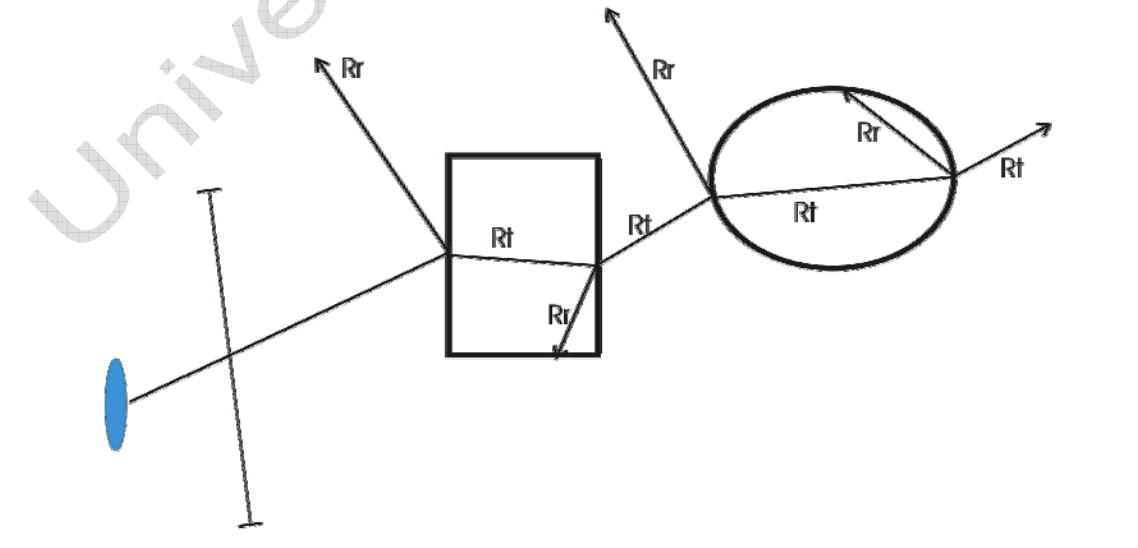
\includegraphics[width=8cm]{Img/CPD/grafica10.jpg}
    \centering
    \caption{\textbf{\footnotesize{ rayos reflejados y transmitidos en ray tracing  }}}
    \label{fig:grafica10}
\end{figure}

En la Figura \ref{fig:grafica10} puede apreciarse el trazado del rayo reflejado y transmitido, en cada punto de intersección. En la misma figura puede verse que cada rayo primario trazado lleva asociado un árbol binario (árbol de rayos) como el mostrado a continuación en la Figura \ref{fig:grafica11}

\begin{figure}[h]
    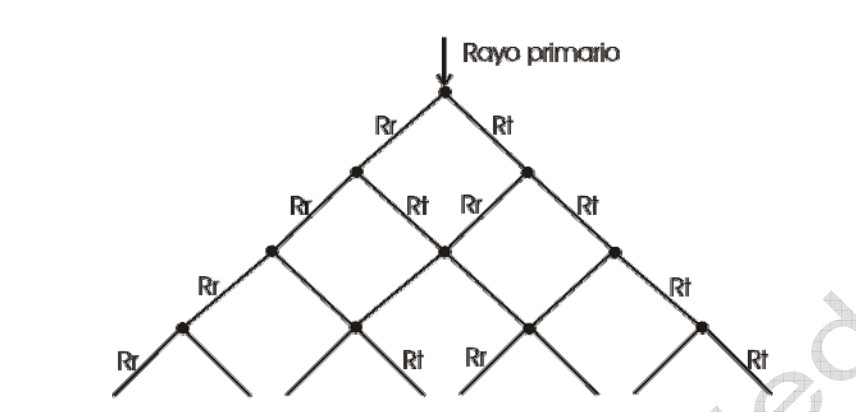
\includegraphics[width=8cm]{Img/CPD/grafica11.jpg}
    \centering
    \caption{\textbf{\footnotesize{  árbol binario asociado a cada rayo primario  }}}
    \label{fig:grafica11}
\end{figure}

A la vista del árbol anterior es fácil comprender la naturaleza recursiva del algoritmo de ray tracing. Por la descripción gráfica que acabamos de ver del algoritmo, los pasos a dar para su desarrollo son:
\begin{enumerate}
    \item Como en ray casting, primero se ha de trazar el rayo primario, es decir, hay que calcular el rayo procedente del ojo que pasa a través de un píxel dado, buscando la intersección más cercana con los objetos del escenario.
\item Una vez encontrado el punto de intersección, para averiguar el \textbf{color global} (final) del rayo primario (y del píxel), se calcula primero la contribución local en el punto de intersección. Para ello es preciso conocer, entre otros datos, qué fuentes aportan luz, y cuales no. Esto se consigue trazando \textbf{rayos de sombra} desde el punto de intersección hacia cada una de las fuentes de luz, evaluando la contribución de cada fuente en función de sus características y de los objetos interpuestos (si los hay) en la trayectoria del correspondiente rayo de sombra (Figura \ref{fig:grafica12a}).
\begin{figure}[h]
    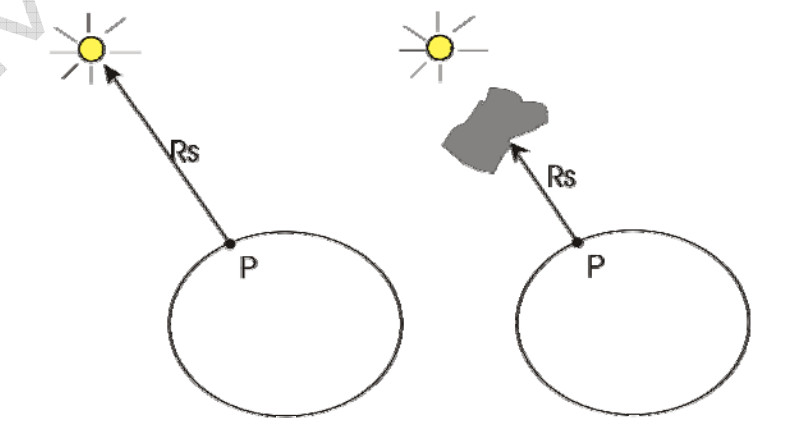
\includegraphics[width=8cm]{Img/CPD/grafica12a.jpg}
    \centering
    \caption{\textbf{\footnotesize{  rayos de sombra para evaluar la \textit{contribución local} en un píxel   }}}
    \label{fig:grafica12a}
\end{figure}
\item En el caso de que la superficie presente reflexión (que es lo más frecuente) calcularemos la trayectoria del rayo reflejado con respecto a la normal a la superficie en el punto de intersección. En el cálculo de esta trayectoria normalmente se supone que el objeto (superficie) es un \textit{reflector perfecto}

\item De la misma forma, si el objeto es transmisor de la luz, se ha de calcular la trayectoria del rayo transmitido hacia el interior del objeto, determinando el ángulo de refracción por la ley de Snell\footnote{\url{https://es.wikipedia.org/wiki/Ley_de_Snell}}
\end{enumerate}

\begin{figure}[h]
    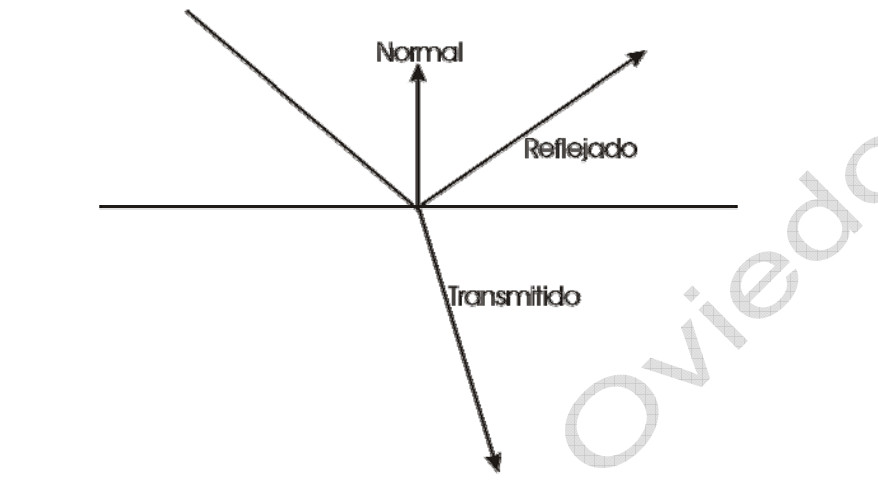
\includegraphics[width=8cm]{Img/CPD/grafica12.jpg}
    \centering
    \caption{\textbf{\footnotesize{  trazado de los rayos reflejado y transmitido   }}}
    \label{fig:grafica12}
\end{figure}


Puesto que en el algoritmo de ray tracing los rayos normalmente se trazan hacia atrás, a continuación se ha de seguir la pista del rayo reflejado (o bien la del transmitido), para encontrar los respectivos puntos de procedencia
de la luz, es decir, los puntos de intersección (más cercanos) con los objetos del escenario. Localizados éstos, de nuevo se generan rayos de sombra (para calcular la contribución local), de transmisión (para hallar la contribución
transmitida) y de reflexión (para la contribución reflejada), todos ellos con origen en los puntos de intersección recién encontrados. Como se puede observar, algorítmicamente se vuelve a una situación similar a la del punto de
partida (aunque no igual), lo que se aconseja es una implantación recursiva del proceso de trazado de los rayos. 

\vskip

El problema principal del algoritmo trazador de rayos es su lentitud, ya que para generar una imagen puede emplear una enorme cantidad de tiempo. Básicamente, esto se debe a que para cada rayo trazado se ha de probar si interseca con cada objeto presente en el escenario. Las principales técnicas de aceleración traten de minimizar el tiempo empleado en la búsqueda de puntos de intersección, aunque este no es el único criterio de aceleración utilizado. Muchos de estos procesos dependen de la tecnología de hardware utilizada ( tarjetas de vídeo, monitores) tanto en los procesos de cálculos geométricos como los de rasterización.
 

Con lo visto en esta sección sobre la Síntesis de Imágenes, es suficiente para tener una idea global sobre este campo de la IG. Si bien en la actualidad se utilizan implementaciones de Radiocity y algoritmos de Pathtracing\footnote{\url{http://madebyevan.com/webgl-path-tracing/}} para generar resultados fotorrealistas\footnote{El fotorrealismo es la cualidad de una imagen generada por computadora que trata de imitar las imágenes generadas por cámaras fotográficas}, en el contexto de este trabajo de investigación se hace incapié en la visualización utilizando \textit{Ray Tracing} ya que los objetivos de calidad de imágenes para el prototipo COCADA son suficientes con este método. Pasamos a continuación a ver una panorámica general del otro campo que se analiza a lo largo de este trabajo: el \textit{Modelado Geométrico de sólidos}.


\clearpage
\section{Modelado Geométrico}

Los modelos son útiles porque permiten hacer estudios sobre objetos que de otra forma sería difícil realizar, ya sea porque aún no existen (no se han fabricado), o por que no son observables directamente (ej. moléculas). Sin embargo, los modelos físicos y matemáticos están limitados al ámbito de su utilidad, de forma que para analizar un nuevo problema normalmente se requiere un nuevo modelo. Se ha intentado solventar este inconveniente dando a los modelos un carácter de generalidad. Tradicionalmente fué el dibujo técnico quien tuvo mayor éxito como técnica de propósito general para describir modelos, ya que los planos se pueden utilizar para extraer información de diversas clases, incluyendo los datos para la formación de modelos físicos y matemáticos.
Sin embargo, con la llegada de los sistemas informáticos el dibujo técnico \footnote{Dibujo geométrico y a escala con fines técnicos o para aplicaciones técnicas.} fué desplazado por los \textit{modelos informáticos}, que gracias a su dinamismo y universalidad superan con creces a cualquier otro tipo de modelado.\vskip

Los modelos informáticos se sirven de la enorme potencia de procesamiento de las computadoras para realizar tareas similares a las que podrían hacerse con los modelos tradicionales, pero aprovechando sus ventajas y evitando inconvenientes. Mediante técnicas y algoritmos desarrollados formalmente, es decir, con una base matemática sólida, se consiguen sistemas de modelado de propósito general que soportan una gran variedad de modelos diferentes, de igual manera que el dibujo técnico.\vskip

La cantidad total de datos que se deben almacenar en un modelo informático, depende del ámbito de las preguntas que algorítmicamente queramos responder a partir del modelo.
Muchos de los problemas a resolver mediante los modelos tienen naturaleza geométrica.
Por ejemplo, el problema de hallar la imagen coloreada de un objeto incluye cuestiones geométricas tales como:
\begin{description}
    \item a) ¿Qué partes del objeto son visibles para el observador?
    \item b) ¿Qué color se debe asignar a cada punto de la imagen?
\end{description}


Si se puede representar en la computadora la forma geométrica de un objeto, se pueden responder a estas preguntas y a muchas otras. De hecho, la información geométrica sobre un objeto es la parte más útil del total de información sobre el objeto. Además, las técnicas para almacenar y procesar la información geométrica son relativamente independientes de un modelo particular. Así, procesos esencialmente iguales de modelado se utilizan en la construcción de modelos de barcos, casas, o zapatos.
Acorde con lo dicho, en un modelo tiene sentido separar la información geométrica de los objetos, de la no geométrica. Bajo este planteamiento, al total de información del modelo informático se conoce como \textit{modelo del objeto}, mientras que \textit{la información exclusivamente geométrica constituye el modelo geométrico} \citep{Ramos2012}.\vskip

Por lo tanto, el concepto de \textit{\textbf{Modelado Geométrico} se refiere al conjunto de métodos utilizados para definir la forma y otras características de los objetos}. La construcción de los objetos es normalmente, en si misma, una operación asistida por ordenador. Éstos juegan un papel primordial, ya que sin su potencia de cálculo los procedimientos del Modelado Geométrico solamente podrían aplicarse en modelos de escasa importancia práctica.
Los métodos del Modelado Geométrico vienen a ser un compendio de las técnicas utilizadas en varias disciplinas, como la Geometría Analítica y Descriptiva, la Topología, la Teoría de Conjuntos, el Análisis Numérico, las Estructuras de Datos, el Cálculo Vectorial y los Métodos Matriciales.\vskip
Se pueden enumerar tres aplicaciones básicas del Modelado Geométrico: 

\begin{itemize}
  \item \textit{Representación} de los objetos existentes.
  \item \textit{Diseño} de los objetos inexistentes y
  \item \textit{Visualización} (rendering) de los objetos.
\end{itemize}
\vskip

El CAD y el CAM, han sido las principales fuerzas de desarrollo del campo del Modelado Geométrico, aunque otras áreas como la Robótica, Reconocimiento de Formas, Inteligencia Artificial, y el Cálculo Estructural (modelos de elementos finitos) han contribuido también ha su desarrollo.

\subsection{Transformaciones geométricas }

\textquote{El conjunto de operaciones elementales que realiza internamente una computadora para conseguir pasar de la representación de un modelo geométrico tridimensional a su imagen en pantalla 2D, pero que para la impresión del observador parezca estar contemplando un sistema de visualización en el mundo real con tres dimensiones 3D, utiliza las transformadas geométricas.} \citep{villamarin2015}

Existen varias transformadas o transformaciones geométricas, sin embargo en este trabajo se revisan matemáticamente el escalamiento, la translación y la rotación.

\subsubsection{Representación}

En el área de la graficación por computadora \footnote{Es el campo de la informática visual donde se utilizan computadoras tanto para generar como para manipular imágenes}, es común encontrar la representación de las ecuaciones de trasformación por medio de matrices, y se pueden encontrar dos tipos de notaciones para representarlas, una es representando las coordenadas de un punto $p$ como \textit{vectores renglón}, en este caso una matriz de transformación $M$ en 2D, multiplica al punto por la derecha para obtener el nuevo punto $p^\prime$. \citep{Matias2007}

\begin{equation}
   p = \begin{bmatrix}
       x_{1} & x_{2}         
     \end{bmatrix}, \ p^{\prime} = \begin{bmatrix}
       x_{1} & x_{2}         
     \end{bmatrix}= p.M  
\end{equation} 
     
La segunda notación es representando las coordenadas de un punto \textit{p} como \textit{vectores columna}, en este caso una matriz de transformación \textit{M}, multiplica al punto por la izquierda para obtener el nuevo punto \textit{p'}.
\begin{equation}
     p = \begin{bmatrix}
       x_{1} \\ x_{2}         
     \end{bmatrix}, \ p^{\prime} = \begin{bmatrix}
       x_{1} \\ x_{2}           
     \end{bmatrix}= p.M 
\end{equation}
     
En este trabajo, se representan los puntos por medio de \textit{vectores renglón}, por lo tanto las matrices de transformación estarán modeladas para multiplicarlas por la derecha, sin embargo se puede obtener una matriz de transformación en la otra notación calculando su transpuesta.
No todas las transformaciones son aplicadas a un punto como una multiplicación de factores, por tal razón se utilizan las \textit{coordenadas homogéneas} para la representación matricial, y de esta forma todas las transformaciones son tratadas como multiplicaciones.
En coordenadas homogéneas, a cada punto 2D se le agrega una tercera coordenada, de esta forma, en lugar de representar los puntos como $p = (x_{1},\ x_{2}) $  son representados como la terna $p = (x_{1},\ x_{2},\ \omega)$ , al mismo tiempo se dice que un par de coordenadas homogéneas $ (x_{1},\ x_{2}) $ y $(x_{1},\ x_{2},\ \omega)$ representan el mismo punto si una es múltiplo de la otra. Por ejemplo, la terna (4, -2, 6) y (8, -4, 12) representan el mismo punto 2D pero en diferentes coordenadas triples, esto significa que cada punto tiene un sinfín de representaciones en coordenadas homogéneas.\vskip
Al menos una de las coordenadas homogéneas tiene que ser distinta de cero, por lo tanto la terna (0, 0, 0) no es válida. Si la coordenada $\omega \neq 0$, la terna $(x_{1},\ x_{2},\ \omega)$ se puede dividir entre $\omega$ y se obtiene $(x_{1}/\omega,\ x_{2}/\omega,\ 1)$ , cuando se realiza esta división, a los valores $x_{1}/ \omega$ y  $x_{2}/ \omega$  se les llama \textit{coordenadas cartesianas} del punto homogéneo. Una
elección conveniente es hacer el valor de
$\omega = 1$, así cada posición 2D es representada con las coordenadas homogéneas $(x_{1}/\omega,\ x_{2}/\omega,\ 1)$. \vskip
En general para cualquier dimensión las coordenadas homogéneas de un punto \textit{p} en \textit{n}D se escribe como $p = (x_{1},\ x_{2},...,x_{2},\omega)$, el cuál es un vector de longitud \textit{n}+1.


\subsubsection{Extensión de las Transformaciones a Otras Dimensiones}
Las trasformaciones geométricas 3D son extensiones de las transformaciones geométricas 2D, pero con la incorporación del eje Z. Muchas de las operaciones matemáticas utilizadas en las transformaciones de escalamiento y translación se extienden fácilmente, pero la rotación no es tan intuitiva y requiere de un poco más de análisis, para comprender su generalización a otras dimensiones y facilitar su comprensión se explica más adelante la rotación 2D.

\subsubsection{Escalamiento 3D}
El escalamiento permite cambiar el tamaño de un objeto expandiéndolo o contrayéndolo en sus dimensiones.
El escalamiento 3D implica el cambio de tamaño de un poliedro, donde cada punto $p = (x_{1},\ x_{2},\ x_{3})$ es transformado por la multiplicación de tres factores de escalamiento: $s_{1}, s_{2}$ y $s_{3}$ a lo largo de los ejes $X_{1},\ X_{2},\ X_{3}$ respectivamente, de esta forma, las coordenadas del nuevo punto $p^{\prime} = (x_{1}{ \prime},\ x_{2}^{ \prime},\ x_{3}^{ \prime})$ se obtienen como:

$$x_{1}{\prime} = x_{1}.s_{1}$$
$$x_{2}{\prime} = x_{2}.s_{2}$$
$$x_{3}{\prime} = x_{3}.s_{3}$$

Sea $s = (s_{1},\ s_{2},\ s_{3})$ el vector de factores de escalamiento, y $S(s)$ la matriz de
escalamiento, en coordenadas homogéneas el escalamiento de un punto $p$ en 3D se puede expresar como el producto matricial
$p^{\prime} = p.S(s)$ , es decir:

\begin{equation}
\begin{array}{rccl}
\left[
\begin{array}{rccl}
x_{1}{\prime} & x_{2}{\prime} & x_{3}{\prime} & 1\\
\end{array}
\right]
\end{array}
=
\begin{array}{rccl}
\left[
\begin{array}{rccl}
x_{1} & x_{2} & x_{3} & 1\\
\end{array}
\right]
\end{array} 
.
\left[
\begin{array}{rccl}
s_{1} & 0 & 0 & 0\\
0 & s_{2} & 0 & 0\\
0 & 0 & s_{3} & 0\\
0 & 0 & 0 & 1\\
\end{array}
\right]   
\end{equation}


\begin{center}
\textbf{\footnotesize{Expresión matricial para el escalamiento 3D.}}
\end{center}


\begin{center}
\begin{figure}[h]
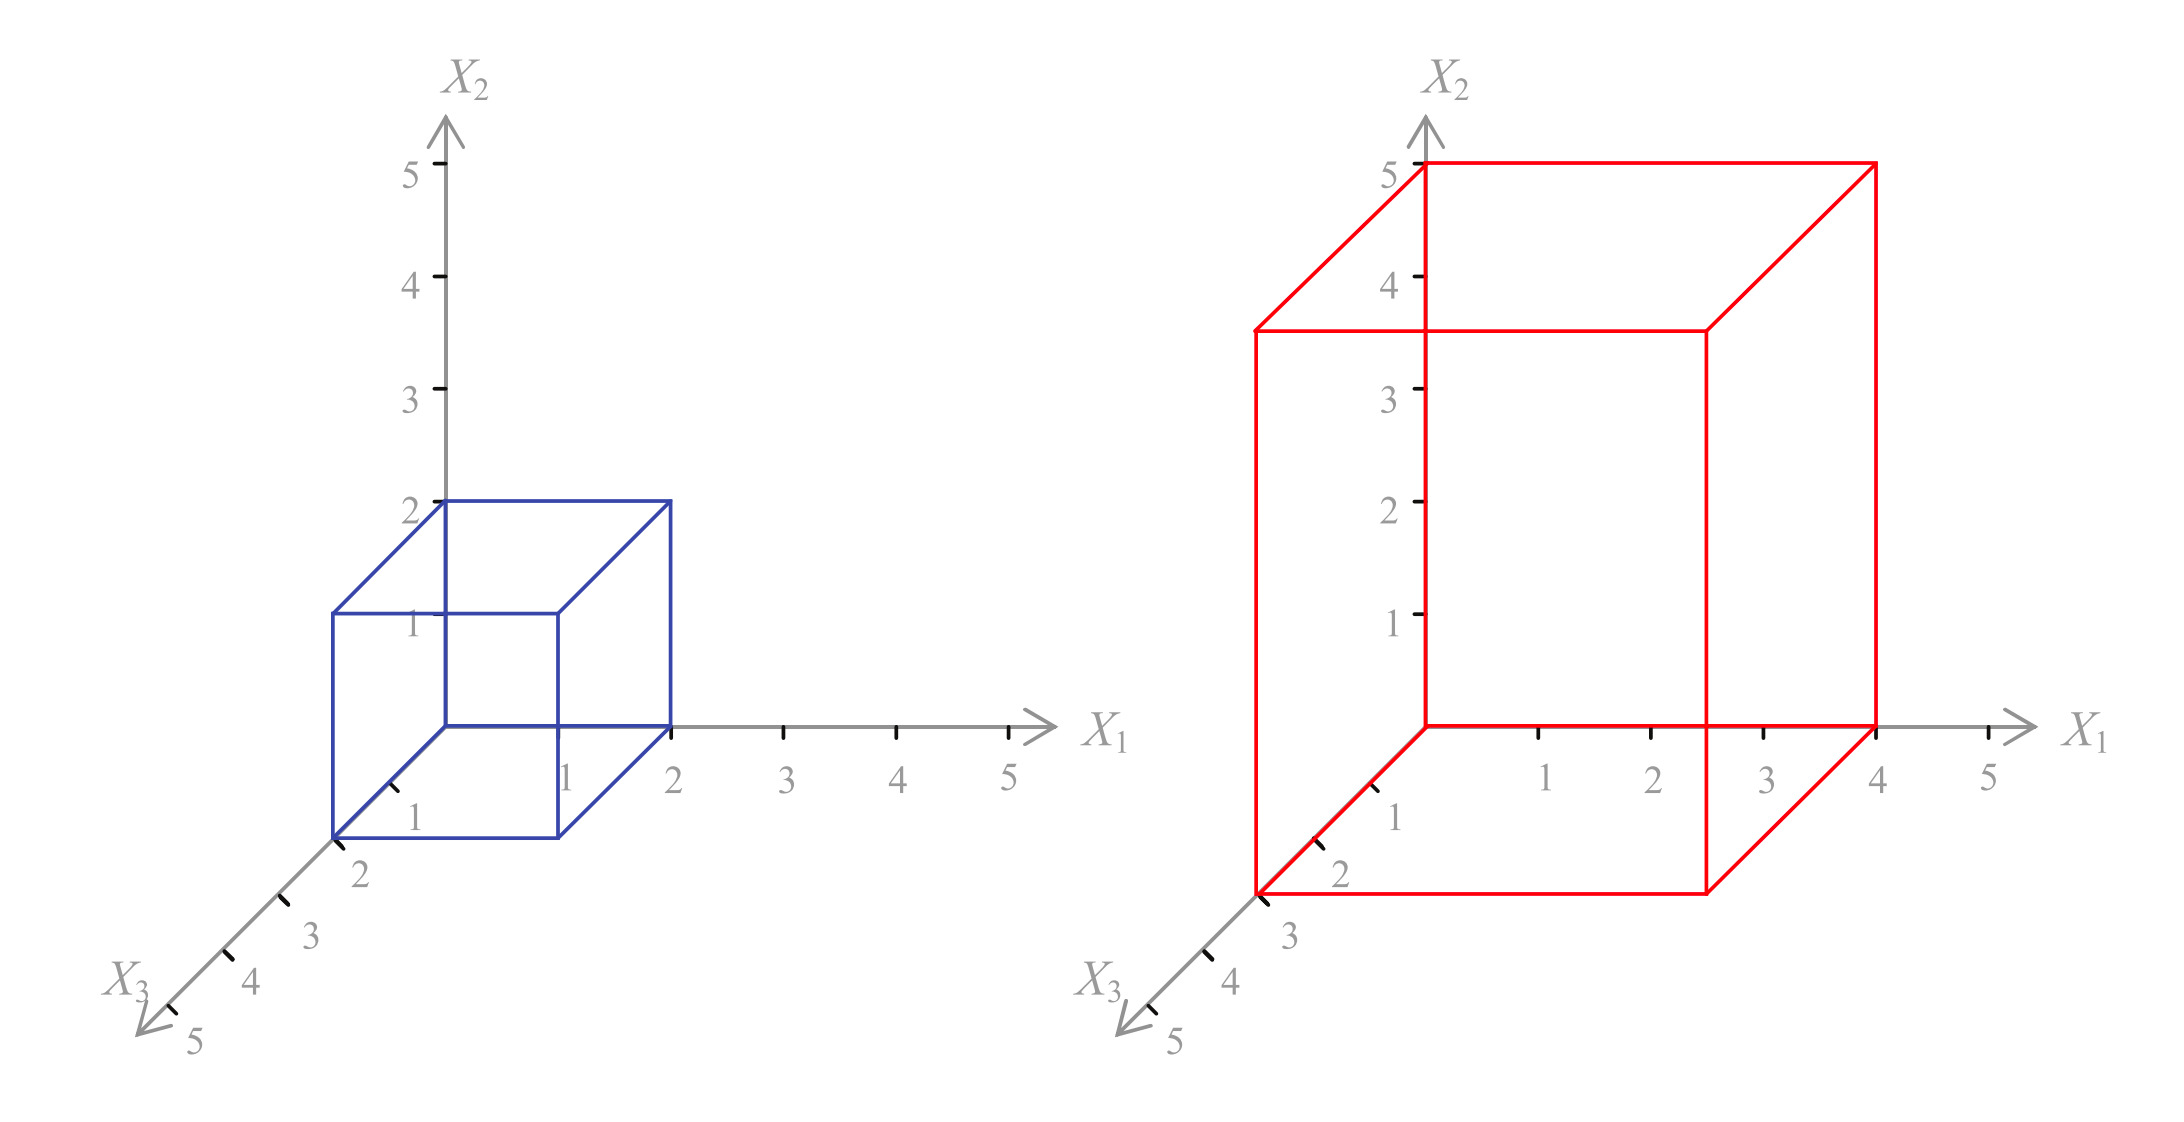
\includegraphics[width=12cm]{Img/GEO/geo-escala.jpg}
\centering
\caption{\textbf{\footnotesize{Efecto de escalamiento de una figura con $s1=2$, $s2=2.5$ y $s3=1.5$}}}
\end{figure}
\end{center}

\subsubsection{Traslación 3D}
La translación permite desplazar un objeto a lo largo de sus dimensiones, como resultado se obtiene un cambio de posición. La translación 3D implica el desplazamiento de un poliedro, donde cada punto $p = (x_{1},\ x_{2},\ x_{3})$ es trasladado $d1$ unidades en el eje $X_1$ , $d_2$ unidades en el eje $X_2$ y $d_3$ unidades en el eje $X_3$, de esta forma, las coordenadas del nuevo punto
$p^{\prime} = (x_{1}{\prime}, \ x_{2}{\prime}, \ x_{3}{\prime})$ se obtienen como:

$$x_{1}{\prime} = x_{1} + d1$$
$$x_{2}{\prime} = x_{2} + d1$$
$$x_{3}{\prime} = x_{3} + d1$$

Sea $d = (d_{1},\ d_{2},\ d_{3})$ el vector de distancias, y $T(d)$ la matriz de translación, en
coordenadas homogéneas la translación de un punto $p$ en 3D se puede expresar como el producto matricial $p^{\prime} = p + T(d)$ , es decir:

\begin{equation}
\begin{array}{rccl}
\left[
\begin{array}{rccl}
x_{1}{\prime} & x_{2}{\prime} & x_{3}{\prime} & 1\\
\end{array}
\right]
\end{array}
=
\begin{array}{rccl}
\left[
\begin{array}{rccl}
x_{1} & x_{2} & x_{3} & 1\\
\end{array}
\right]
\end{array} 
.
\left[
\begin{array}{rccl}
1 & 0 & 0 & 0\\
0 & 1 & 0 & 0\\
0 & 0 & 1 & 0\\
d_{1} & d_{2} & d_{3} & 1\\
\end{array}
\right]
\end{equation}

\begin{center}
\textbf{\footnotesize{Expresión matricial para la traslación 3D.}}
\end{center}

\begin{center}
\begin{figure}[h]
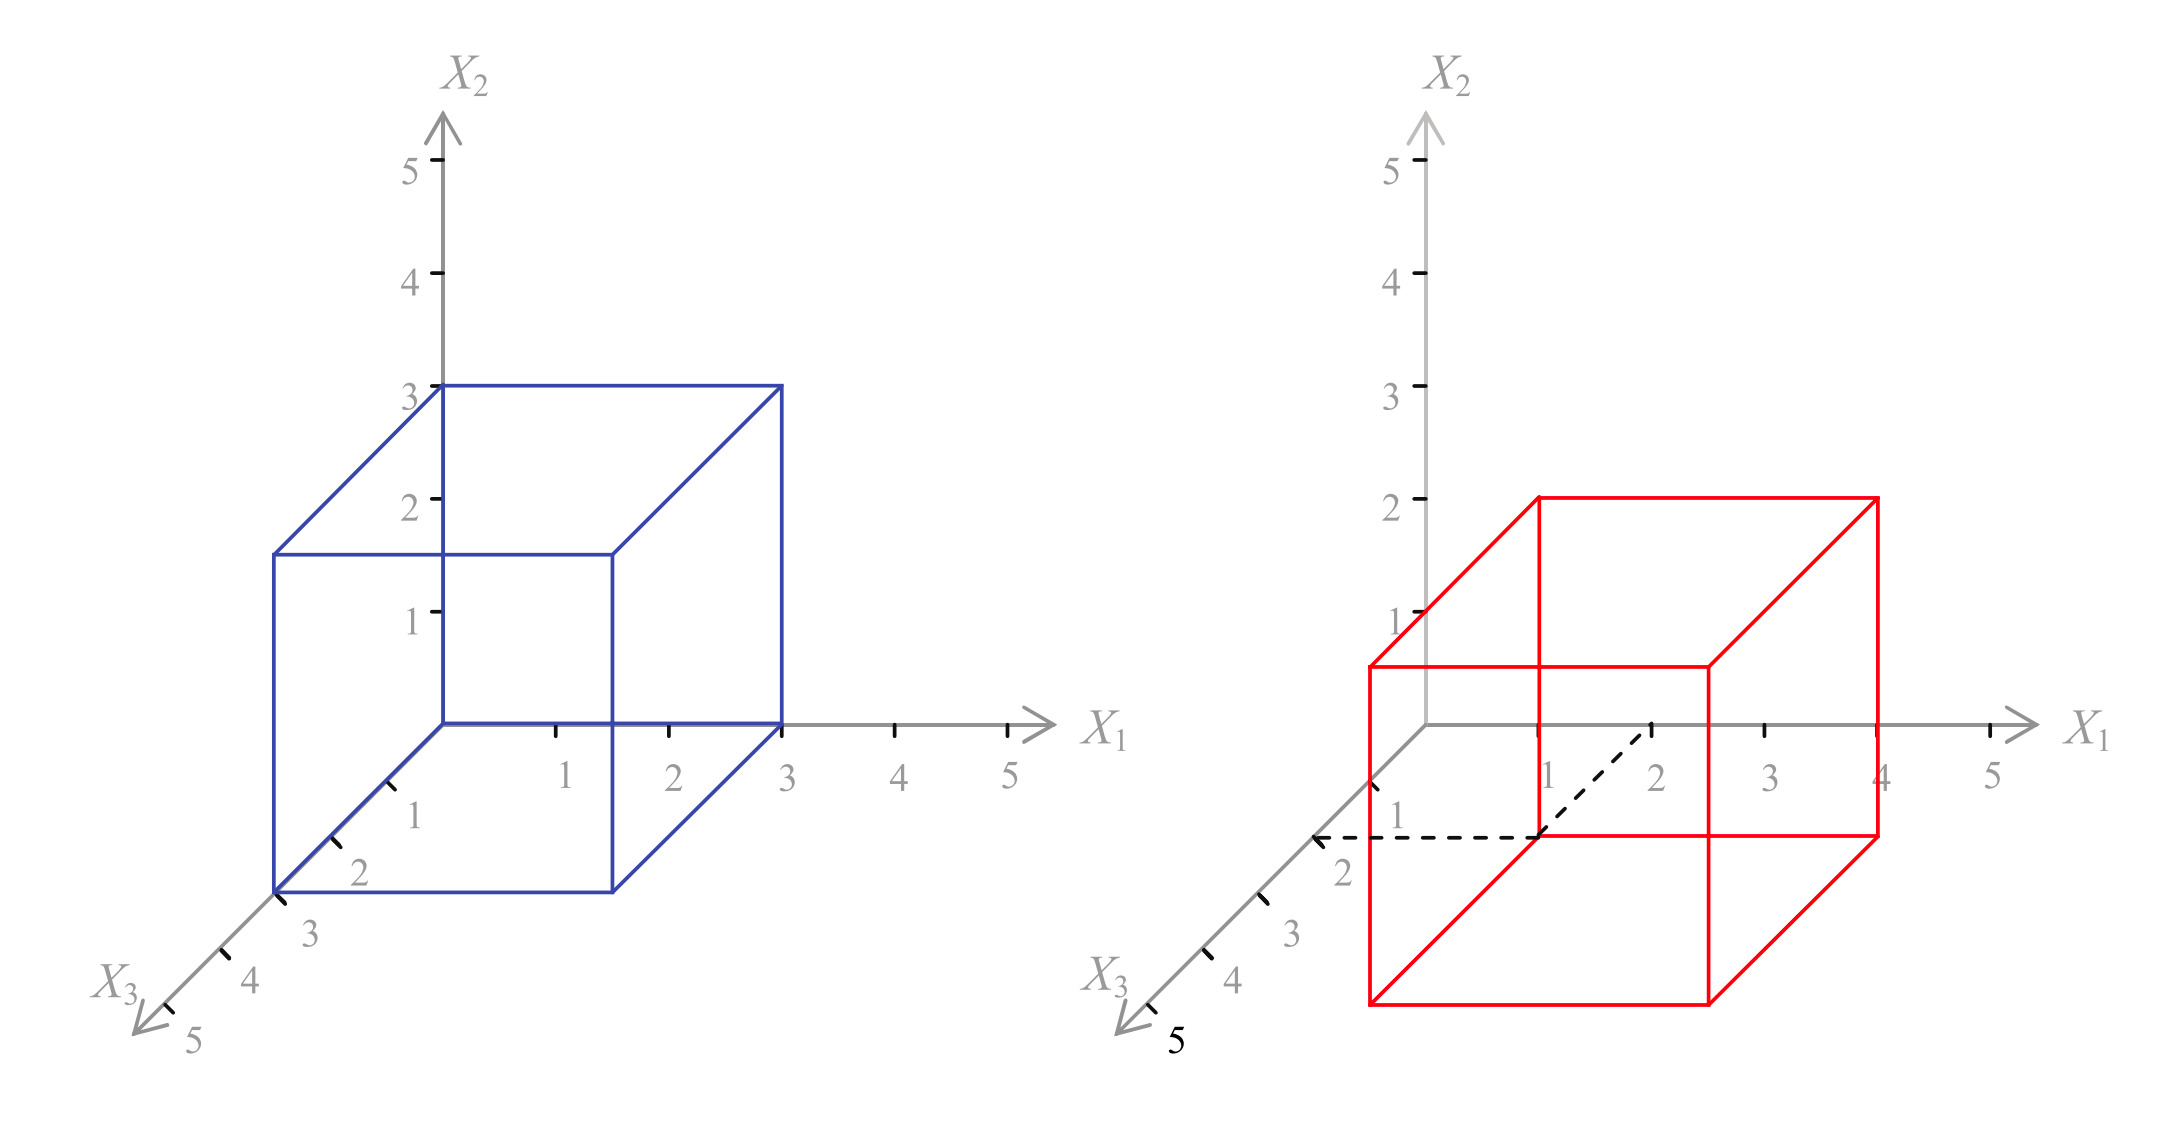
\includegraphics[width=12cm]{Img/GEO/geo-traslacion.jpg}
\centering
\caption{\textbf{\footnotesize{efecto de translación de una figura con $d_1=2$, $d_2=0$ y $d_3=2$}}}
\end{figure}
\end{center}

\subsubsection{Rotación 2D}
La rotación permite girar un objeto sobre un eje de rotación, dado un valor de ángulo de rotación $\theta$ y su dirección. La rotación de un objeto en 2D se lleva a cabo alrededor de un punto, que es el eje
puntual (cero-dimensional) de rotación.\vskip
Para generar una rotación, se especifica el ángulo de rotación , y el punto de rotación $\theta$ (pivote) sobre el cuál el objeto será rotado. Los ángulos de rotación positivos definen una rotación en sentido contrario a las agujas del reloj o sentido antihorario sobre el punto pivote (del eje $X_1$ al eje $X_2$), entonces los ángulos de rotación negativos producen una rotación en el sentido de las agujas del reloj o sentido horario (del eje $X_2$ al eje $X_1$). La rotación 2D es el giro sobre el eje de rotación que es perpendicular al plano $X_1 X_2$ (mejor conocido como plano XY) y que pasa a través del punto pivote.\vskip
Si el punto pivote se encuentra sobre el origen, se tiene que: $r$ es la distancia del punto $p = (x_{1}, \ x_{2})$ al origen, $\phi$ define la posición angular del punto p desde la horizontal, y θ el ángulo de rotación de $p$ para producir el nuevo punto $p^{\prime} = ({x_{1}}^{\prime},\ {x_{2}}^{\prime})$

\begin{center}
\begin{figure}[h]
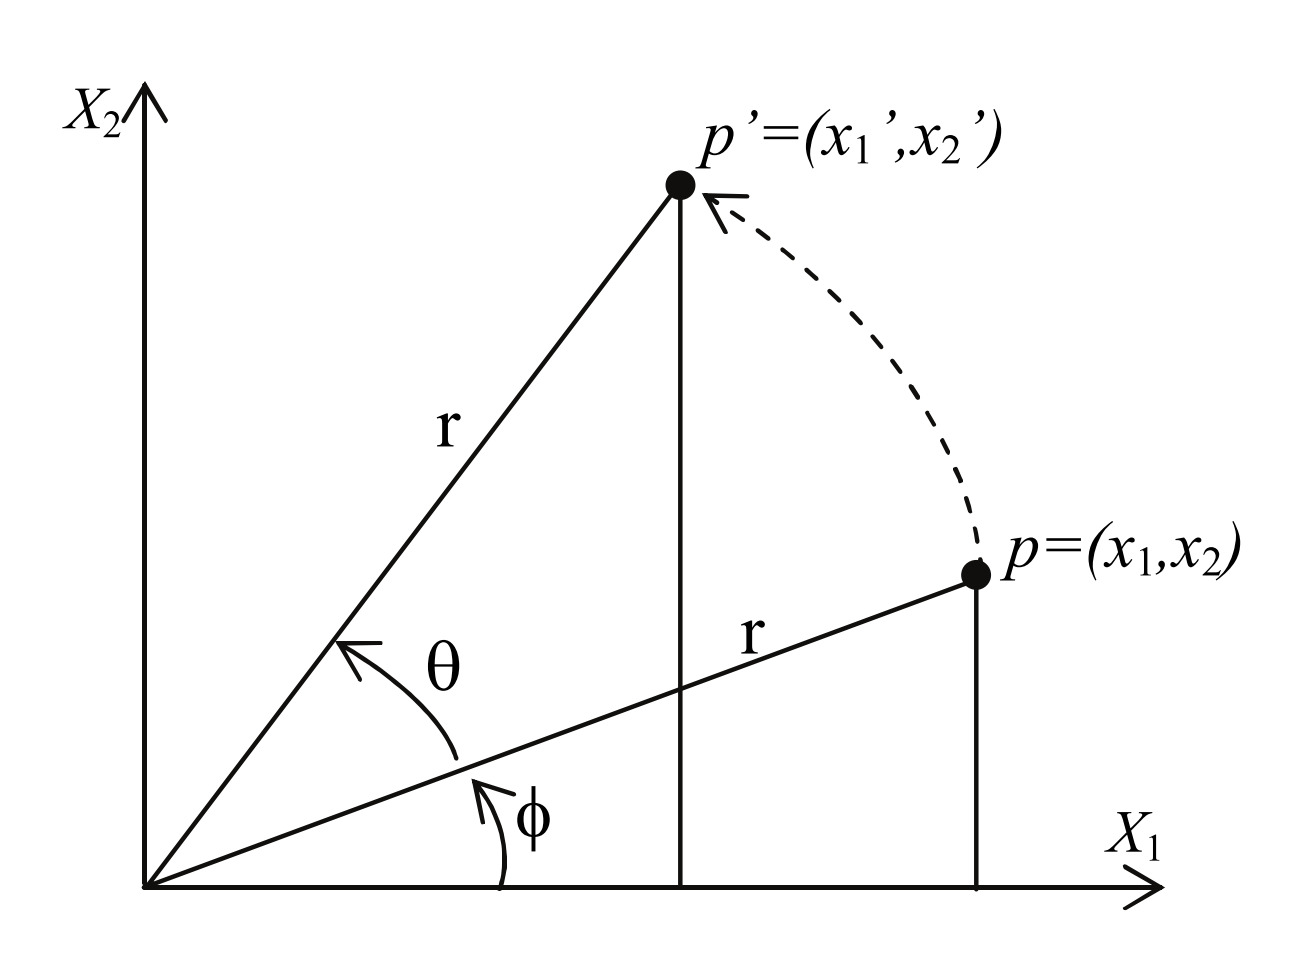
\includegraphics[width=8cm]{Img/GEO/geo-rotacion2d.jpg}
\centering
\caption{\textbf{\footnotesize{Rotación de un punto en 2D alrededor del origen.}}}
\end{figure}
\end{center}

Utilizando coordenadas polares, el punto $p = (x_{1}, \ x_{2})$ se puede escribir como $p = (r, \ \phi)$ y el punto $p^{\prime} = ({x_{1}}^{\prime},\ {x_{2}}^{\prime})$ como $p^{\prime} = (r, \ \phi + \theta)$. Pasando después estos puntos de coordenadas polares a rectangulares se tiene que:

$$
\begin{array}{rccl}
x_{1} = r \cos(\phi)  & x_{2} = r \sin(\phi)\\
{x_{1}}^{\prime} = r \cos(\phi + \theta)  & {x_{2}}^{\prime} = r \sin(\phi + \theta)
\end{array}
$$

Aplicando algunas propiedades trigonométricas:
$$
{x_{1}}^{\prime} = r \cos(\theta + \phi) = r \cos \phi \cos \theta - r \sin \phi \sin \theta
$$
$$
{x_{2}}^{\prime} = r \sin(\theta + \phi) = r \cos \phi \cos \theta - r \sin \phi \sin \theta
$$

Substituyendo los valores de $x_{1} = r \cos(\phi)$ y $x_{2} = r \sin(\phi)$ se obtienen las ecuaciones para rotar un punto $p = (x_{1}, \ x_{2})$ alrededor del origen dado un ángulo $\theta$

\begin{equation}
\begin{cases}
{x_{1}}^{\prime} = x_{1} \cos(\theta) -x_{2} \sin(\theta) \\ 
{x_{2}}^{\prime} = x_{1} \sin(\theta) -x_{2} \cos(\theta)
\end{cases}
\end{equation}

\begin{center}
\textbf{\footnotesize{Fórmulas para la rotación 2D alrededor del origen.}}
\end{center}

Sea $R(\theta)$ la matriz de rotación sobre el origen, en coordenadas homogéneas la
rotación de un punto p alrededor del origen en 2D se puede expresar como el producto matricial $p^{\prime} = p.R(\theta)$, es decir:

\begin{equation}
\begin{array}{rccl}
\left[
\begin{array}{rccl}
x_{1}{\prime} & x_{2}{\prime} & 1\\
\end{array}
\right]
\end{array}
=
\begin{array}{rccl}
\left[
\begin{array}{rccl}
x_{1} & x_{2} &  1\\
\end{array}
\right]
\end{array} 
.
\left[
\begin{array}{rccl}
\cos\theta & \sin\theta & 0\\
-\sin\theta & \cos\theta & 0\\
0 & 0 & 1\\
\end{array}
\right]
\end{equation}

\begin{center}
\textbf{\footnotesize{Expresión matricial para la rotación 2D.}}
\end{center}


\begin{figure}[h]
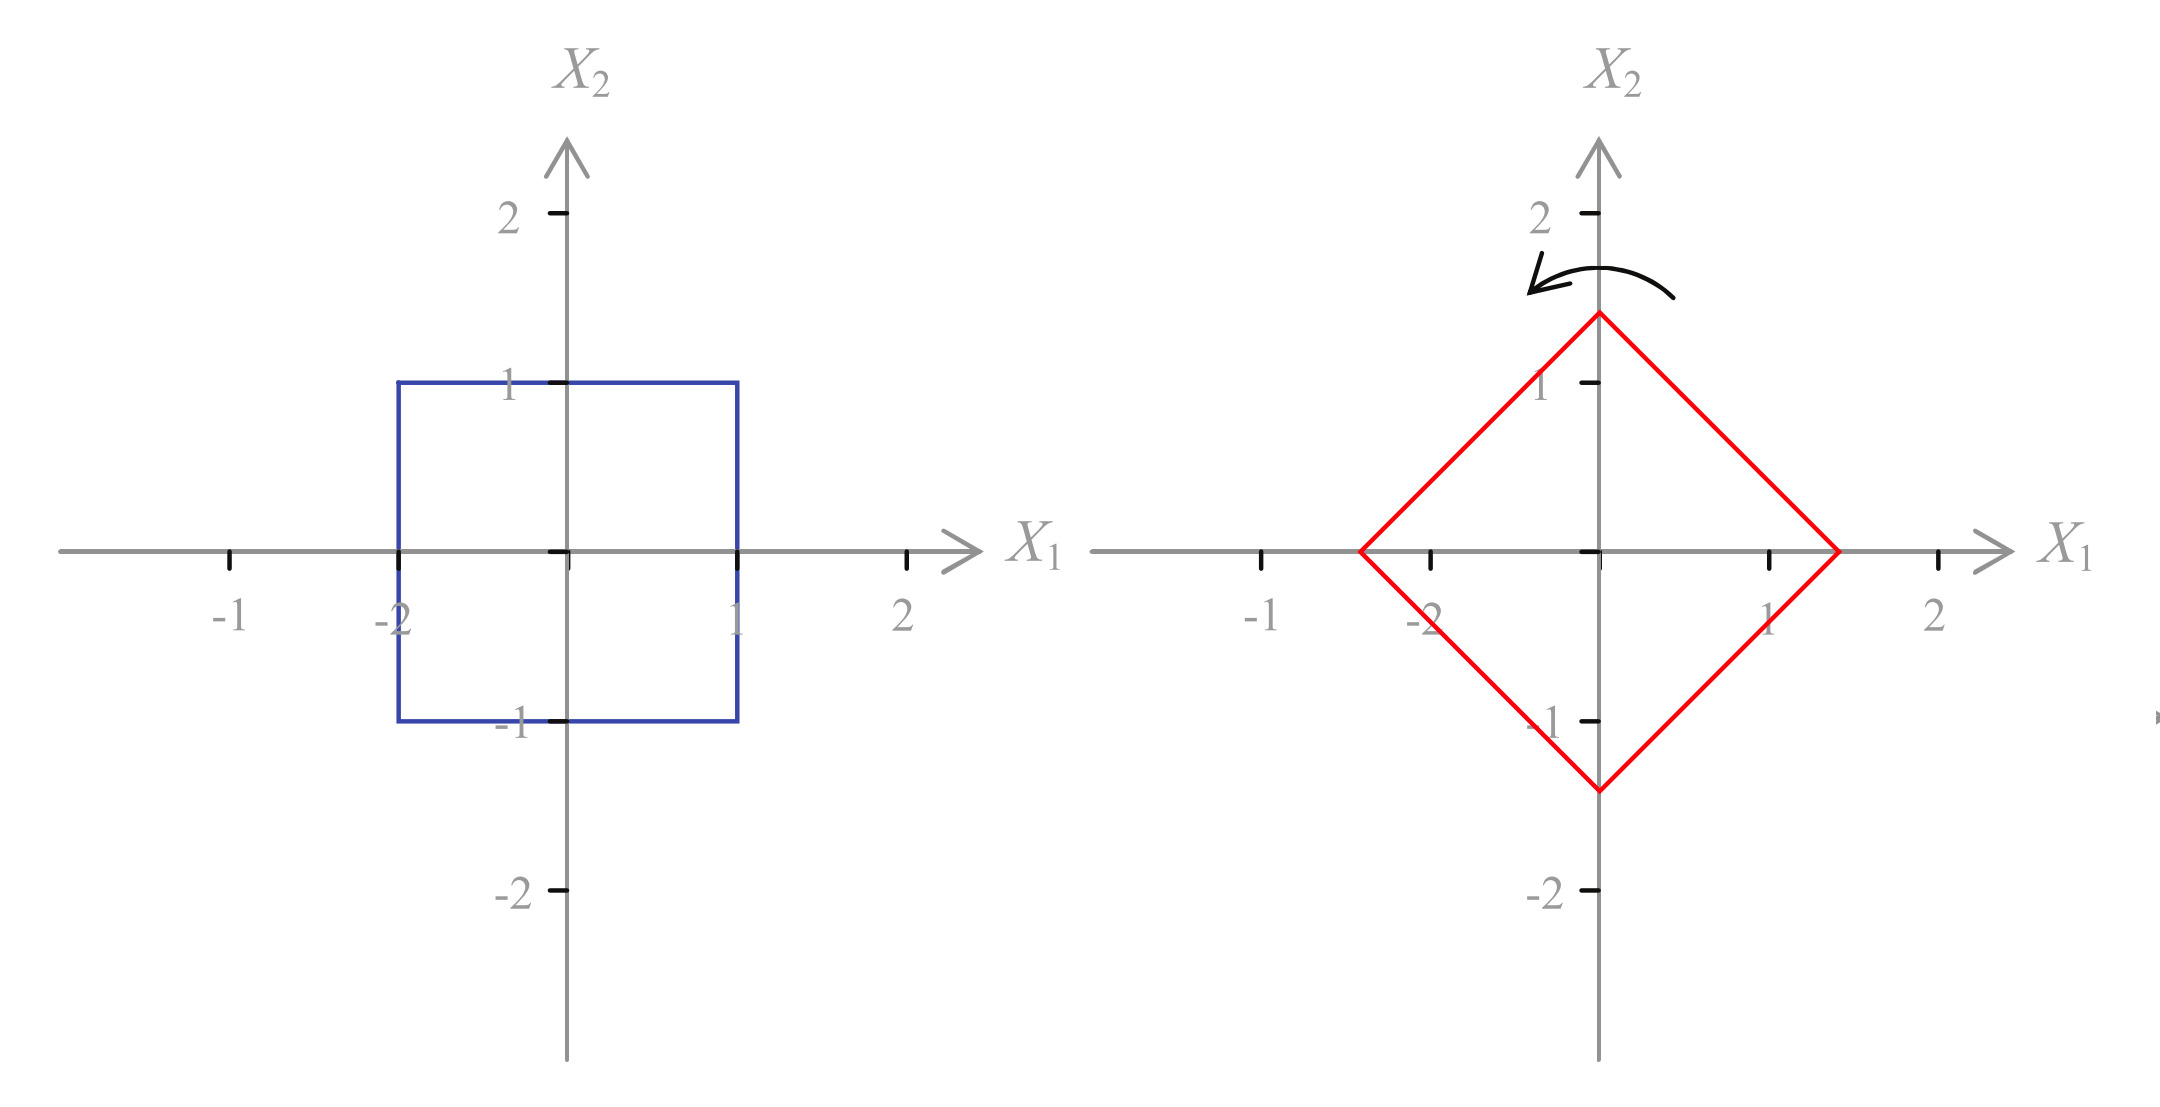
\includegraphics[width=12cm]{Img/GEO/geo-rotacion2d45.jpg}
\centering
    \caption{\footnotesize{\textbf{Ejemplo de rotación 2D con $\theta = 45^{\circ}$}}}
\end{figure}


\clearpage
\subsubsection{Rotaciones principales 3D}

A diferencia de la rotación en el espacio 2D, donde para hacer rotar un objeto se necesita un punto (cero-dimensional), en 3D para hacer rotar un objeto se necesitan dos puntos no coincidentes que determinan un segmento de recta, cuya línea de soporte define un eje lineal (uni-dimensional) de rotación.\vskip
Las \textit{rotaciones principales} 3D, son aquellas cuando el eje de rotación se encuentra sobre alguno de los tres ejes principales: $X_{1}$, $X_{2}$ o $X_{1}$, las rotaciones sobre cualquier otro eje arbitrario son llamadas \textit{rotaciones generales} 3D. Se recuerda que inicialmente, se analizan las rotaciones principales.
Por convención, los ángulos de rotación positivos producen rotaciones en contra de
las agujas del reloj (antihorario) sobre el eje de rotación, esto es si se observa el giro desde la parte positiva del eje hacia el origen. Otra forma de determinar la dirección de un giro positivo es mediante la \textbf{regla de la mano derecha} (Figura 2.4), que dice que: \textit{“Si se coloca el dedo pulgar de la mano derecha sobre el eje de rotación apuntando hacia la parte positiva de dicho eje, el giro natural del resto de los dedos indica la dirección positiva del giro”.}

\begin{figure}[h]
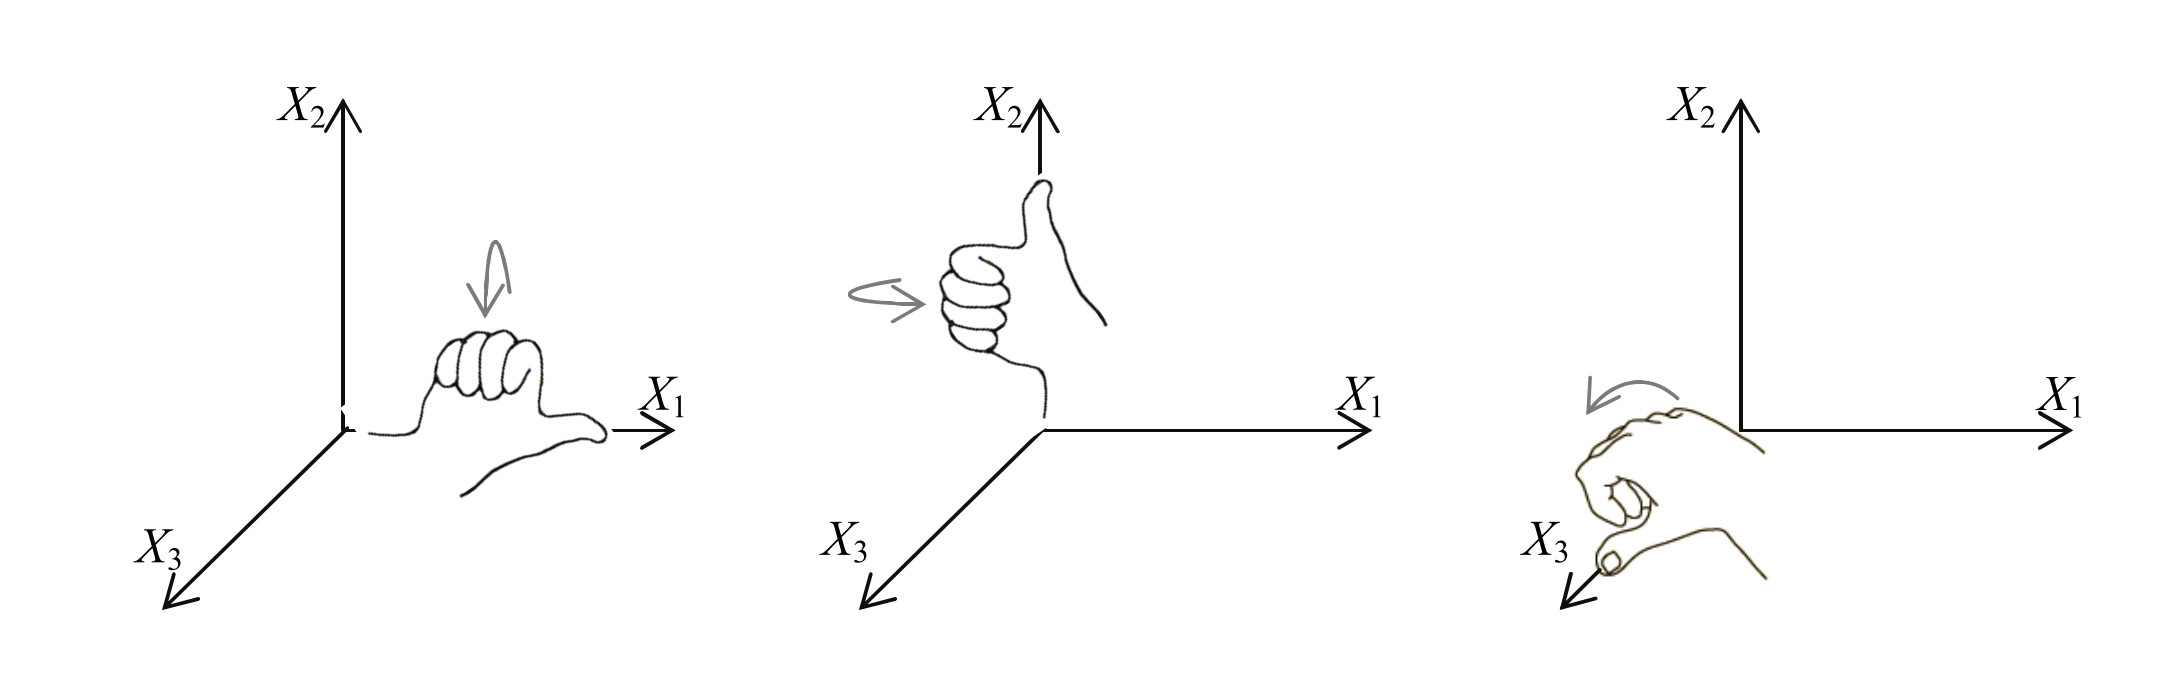
\includegraphics[width=14cm]{Img/GEO/geo-mano.jpg}
\centering
\caption{\textbf{\footnotesize{Regla de la mano derecha para obtener la dirección de un giro positivo en 3D.}}}
\end{figure}

Para entender el concepto de rotación en 3D como una extensión de la rotación 2D, hay que recordar que la rotación 2D es el giro sobre el eje de rotación, que es perpendicular al plano $X_{1}X_{2}$, el cual en 3D corresponde al eje $X_{3}$, entonces se obtiene la primera de las rotaciones principales.
De esta forma, por cada punto
$p = (x_{1},\ x_{2}^,\ x_{3})$ dado un ángulo $\theta$, puede ser rotado sobre el eje X3 en sentido contrario a las agujas del reloj, obteniendo las coordenadas del nuevo punto $p^{\prime} = (x_{1}^{\prime},\ x_{2}^{\prime},\ x_{3}^{\prime})$ de la misma forma en como se analizó en el espacio 2D quedando la coordenada x3 sin cambio, entonces, se extienden las formulas para la rotación 2D a 3D como: 

\begin{equation}\label{eq:giro2d}
\begin{cases}
{x_{1}}^{\prime} = x_{1} \cos(\theta) -x_{2} \sin(\theta) \\ 
{x_{2}}^{\prime} = x_{1} \sin(\theta) +x_{2} \cos(\theta) \\
{x_{3}}^{\prime} = x_{3}
\end{cases}
\end{equation}

\begin{center}
\textbf{\footnotesize{Fórmulas para la rotación 3D alrededor del eje $X_{3}$.}}
\end{center}

Sea $R_{3}(\theta)$ la matriz de rotación alrededor del eje $X_{3}$, en coordenadas homogéneas la rotación de un punto $p$ alrededor de dicho eje, se puede expresar como el producto matricial
$p^{\prime} = p.R_{3}(\theta)$, es decir:



\begin{equation}
\begin{array}{rccl}
\left[
\begin{array}{rccl}
{x_{1}}^{\prime} & {x_{2}}^{\prime} & {x_{3}}^{\prime} & 1\\
\end{array}
\right]
\end{array}
=
\begin{array}{rccl}
\left[
\begin{array}{rccl}
x_{1} & x_{2} & x_{3} & 1\\
\end{array}
\right]
\end{array} 
.
\left[
\begin{array}{rccl}
\cos\theta & \sin\theta & 0 & 0\\
-\sin\theta & \cos\theta & 0 & 0\\
0 & 0 & 1 & 0\\
0 & 0 & 0 & 1\\
\end{array}
\right]
\end{equation}

\begin{center}
\textbf{\footnotesize{Expresión matricial para la rotación 3D alrededor del eje $X_{3}$}}
\end{center}

\begin{figure}[h]
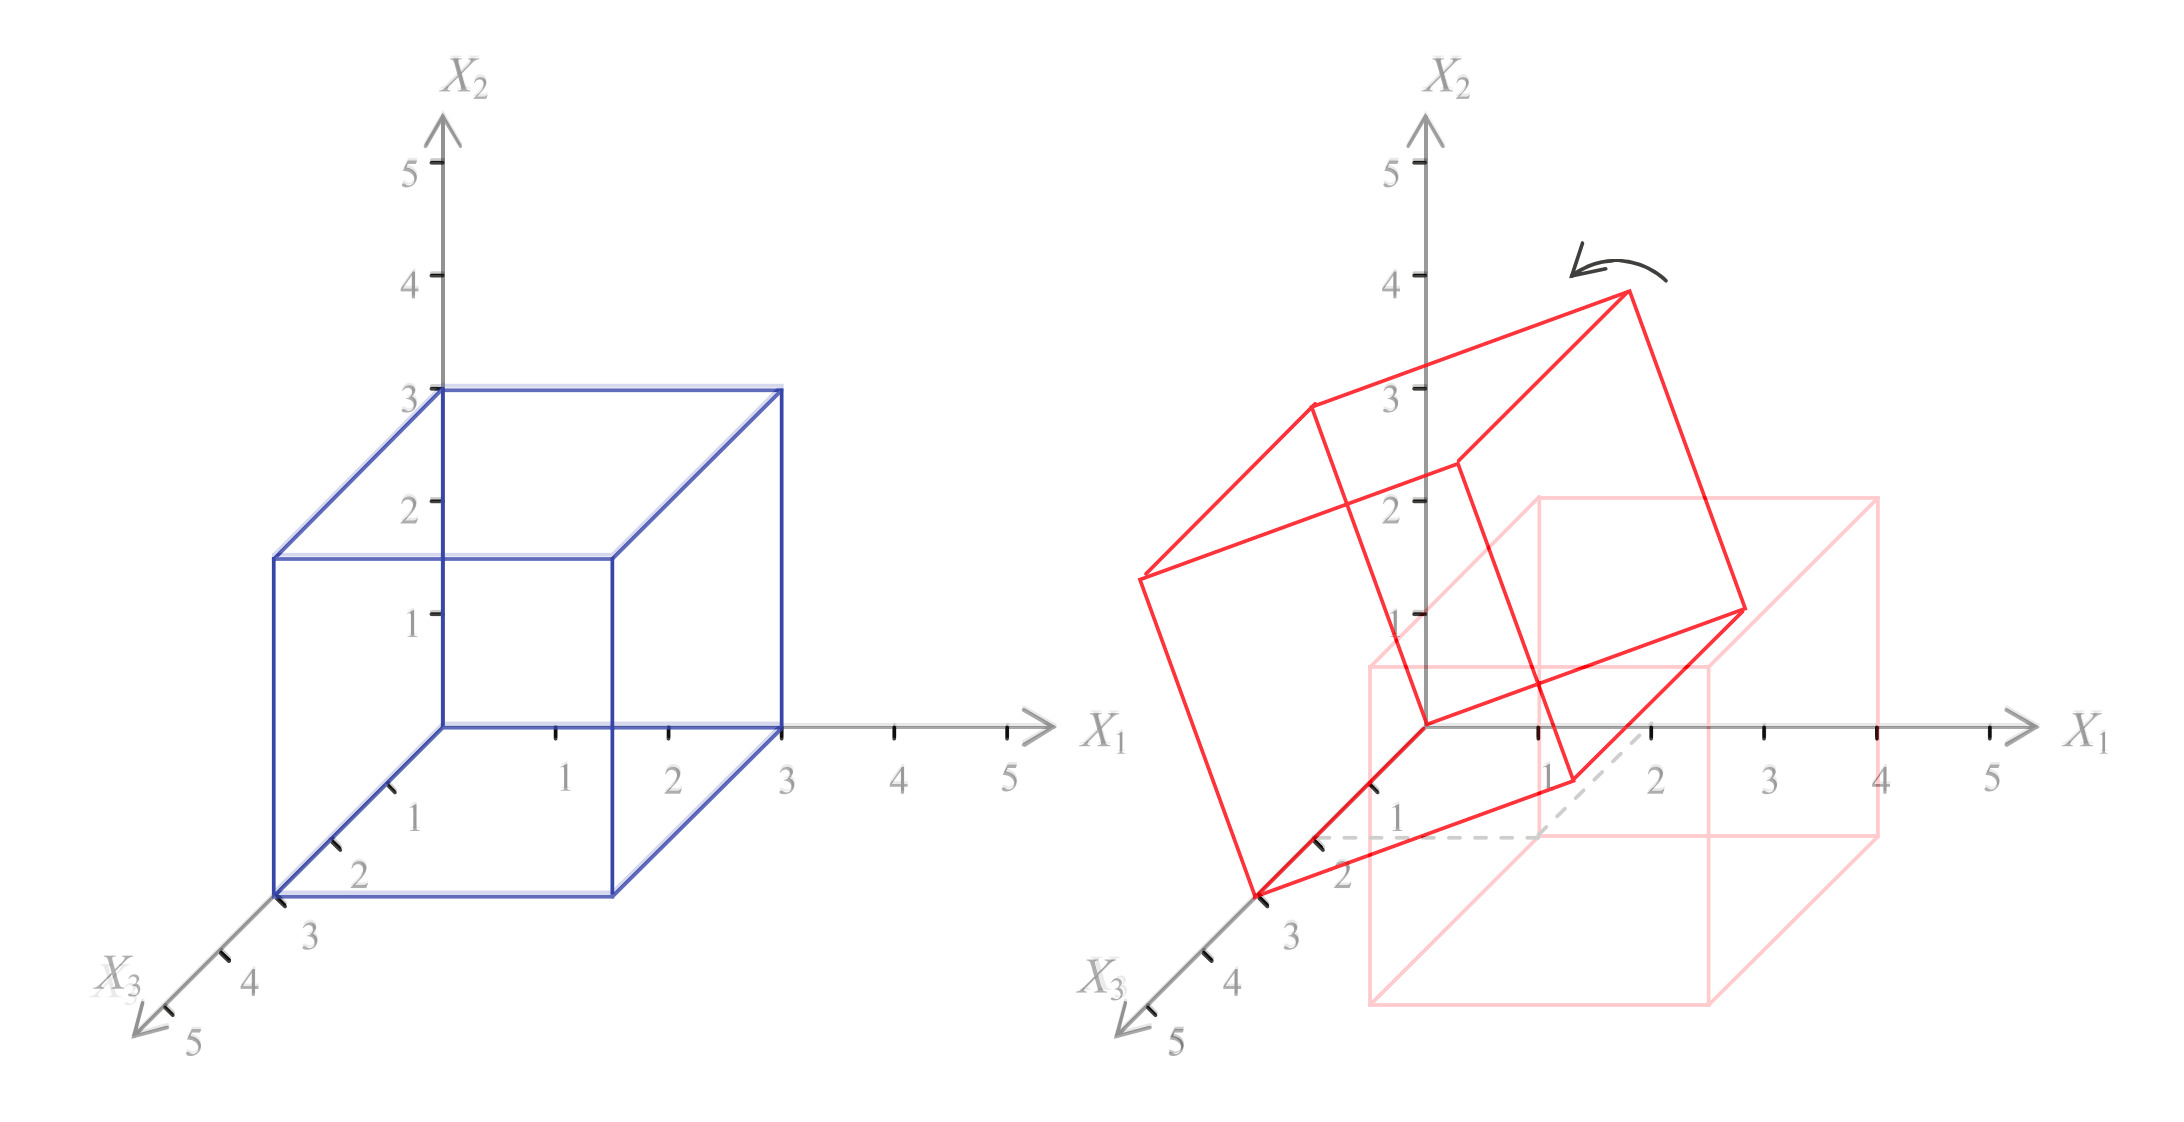
\includegraphics[width=12cm]{Img/GEO/geo-rotacion3d.jpg}
\centering
    \caption{\footnotesize{\textbf{Ejemplo de rotación sobre el eje $X_{3}$ de una figura con $\theta = 20^{\circ}$}}}
\end{figure}

Las ecuaciones para las rotaciones sobre el eje $X_{1}$, y eje $X_{2}$, pueden ser obtenidas mediante las permutaciones cíclicas de los parámetros $X_{1}$, $X_{2}$, $X_{3}$: \vskip
\begin{center}
$X_{1}$\xrightarrow{}$X_{2}$\xrightarrow{}$X_{3}$
\end{center}

\begin{figure}[h]
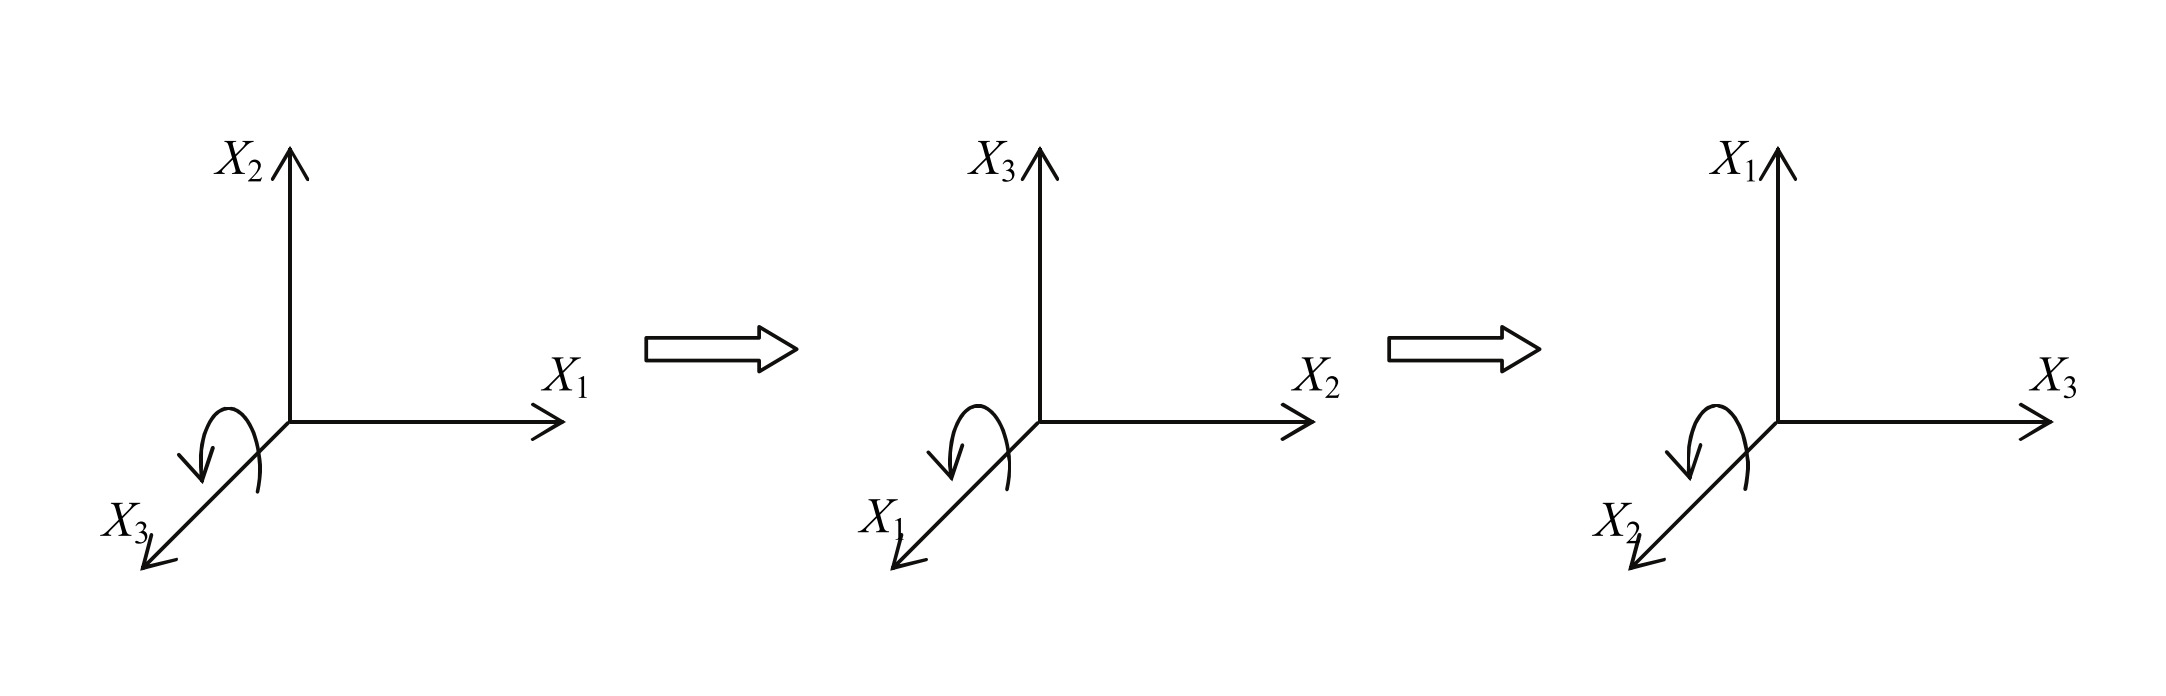
\includegraphics[width=12cm]{Img/GEO/geo-trans.jpg}
\centering
    \caption{\footnotesize{\textbf{Permutaciones cíclicas de los ejes coordenados}}}
\end{figure}



Entonces, aplicando estas substituciones cíclicas en la \ref{eq:giro2d}, se obtienen las ecuaciones para la rotación alrededor del eje $X_{1}$ dado un ángulo
$\theta$


\begin{equation}\label{eq:giro2d1}
  \begin{split}
   \begin{cases}
{x_{2}}^{\prime} = x_{2} \cos(\theta) -x_{3} \sin(\theta) \\ 
{x_{3}}^{\prime} = x_{2} \sin(\theta) +x_{3} \cos(\theta) \\
{x_{1}}^{\prime} = x_{1}
\end{cases}
  \end{split}
\quad\longrightarrow\quad
  \begin{split}
   \begin{cases}
{x_{1}}^{\prime} = x_{1} \\ 
{x_{2}}^{\prime} = x_{2} \cos(\theta) -x_{3} \sin(\theta) \\
{x_{3}}^{\prime} = x_{2} \sin(\theta) +x_{3} \cos(\theta)
\end{cases}
\end{split}
\end{equation}

\begin{center}
\textbf{\footnotesize{Fórmulas para la rotación 3D alrededor del eje $X_{1}$}}
\end{center}
    
Sea $R_{1}( \theta )$ la matriz de rotación alrededor del eje $X_{1}$, en coordenadas homogéneas la
rotación de un punto p alrededor de dicho eje, se puede expresar como el producto matricial $p^{\prime} = p.R_{1}(\theta)$, es decir:

\begin{equation}
\begin{array}{rccl}
\left[
\begin{array}{rccl}
{x_{1}}^{\prime} & {x_{2}}^{\prime} & {x_{3}}^{\prime} & 1\\
\end{array}
\right]
\end{array}
=
\begin{array}{rccl}
\left[
\begin{array}{rccl}
x_{1} & x_{2} & x_{3} & 1\\
\end{array}
\right]
\end{array} 
.
\left[
\begin{array}{rccl}
1 & 0 & 1 & 0\\
0 & \cos\theta & \sin\theta &  0\\
0 & -\sin\theta & \cos\theta & 0 \\
0 & 0 & 0 & 1\\
\end{array}
\right]
\end{equation}

\begin{center}
\textbf{\footnotesize{Expresión matricial para la rotación 3D alrededor del eje $X_{1}$}}
\end{center}

Aplicando nuevamente las substituciones cíclicas en la \ref{eq:giro2d1}, se obtienen las fórmulas para la rotación alrededor del eje $X_{2}$ dado un ángulo $\theta$

\begin{equation}
  \begin{split}
   \begin{cases}
{x_{3}}^{\prime} = x_{3} \cos(\theta) -x_{1} \sin(\theta) \\ 
{x_{1}}^{\prime} = x_{3} \sin(\theta) +x_{1} \cos(\theta) \\
{x_{2}}^{\prime} = x_{2}
\end{cases}
  \end{split}
\quad\longrightarrow\quad
  \begin{split}
   \begin{cases}
{x_{1}}^{\prime} = x_{1} \cos(\theta) + x_{3}\sin(\theta) \\ 
{x_{2}}^{\prime} = x_{2} \\
{x_{3}}^{\prime} = -x_{1} \sin(\theta) + x_{3} \cos(\theta)
\end{cases}
\end{split}
\end{equation}

\begin{center}
\textbf{\footnotesize{Fórmulas para la rotación 3D alrededor del eje $X_{2}$}}
\end{center}


Sea $R_{2}( \theta )$ la matriz de rotación alrededor del eje $X_{2}$, en coordenadas homogéneas la rotación de un punto p alrededor de dicho eje, se puede expresar como el producto matricial $p^{\prime} = p.R_{2}(\theta)$, es decir:

\begin{equation}
\begin{array}{rccl}
\left[
\begin{array}{rccl}
{x_{1}}^{\prime} & {x_{2}}^{\prime} & {x_{3}}^{\prime} & 1\\
\end{array}
\right]
\end{array}
=
\begin{array}{rccl}
\left[
\begin{array}{rccl}
x_{1} & x_{2} & x_{3} & 1\\
\end{array}
\right]
\end{array} 
.
\left[
\begin{array}{rccl}
1 & 0 & 1 & 0\\
0 & \cos\theta & \sin\theta &  0\\
0 & -\sin\theta & \cos\theta & 0 \\
0 & 0 & 0 & 1\\
\end{array}
\right]
\end{equation}

\begin{center}
\textbf{\footnotesize{Expresión matricial para la rotación 3D alrededor del eje $X_{2}$}}
\end{center}

\subsubsection{Rotaciones 3D Como Rotaciones Paralelas a un Plano}

Las rotaciones en el espacio 3D son bien conocidas y entendidas por la mayoría de la
gente, y muchos pueden interpretarla como la rotación de un objeto alrededor de un eje (uni-dimensional) de rotación, sin embargo, es más adecuado pensar en un conjunto de rotaciones paralelas a un plano 2D, inmerso en el espacio. Se sabe que en 3D hay tres ejes coordenados: $X_1$, $X_2$ y $X_3$, y los planos principales son los formados por todas las posibles combinaciones de 2 de estos ejes, se obtienen así, los planos principales 3D: $X_1X_2$, $X_1X_3$ y $X_2X_3$.\vskip
Como se ve en la explicaciones anteriores, hay tres rotaciones principales, alrededor de cada uno los ejes principales, y durante estos giros se cumple que: dado el origen y ángulo de rotación, el conjunto de todos los puntos rotados por una matriz dada caen en un plano, llamado \textit{plano de rotación}, y el eje lineal de rotación es el que coincide con el vector normal de este plano. Esto es consistente con el espacio 2D, porque todos los puntos rotados caen en un único y mismo plano, el plano $X_1X_2$. \vskip
Entonces se puede deducir que las rotaciones alrededor de los ejes coordenados producen rotaciones de todos los planos paralelos al plano de rotación, el cuál está formado por los ejes restantes, es decir, si el eje de rotación es el eje $X_3$, el plano de rotación será el formado por los ejes coordenados restantes: el plano $X_1X_2$, de esta manera, si el eje de rotación es el eje $X_2$, el plano de rotación será el plano $X_1X_3$, y si el eje de rotación es el eje $X_1$, y el plano de rotación será el plano $X_2X_3$ (ver Figura \ref{rotaciones} a) b) y c) respectivamente).


\begin{figure}[h]
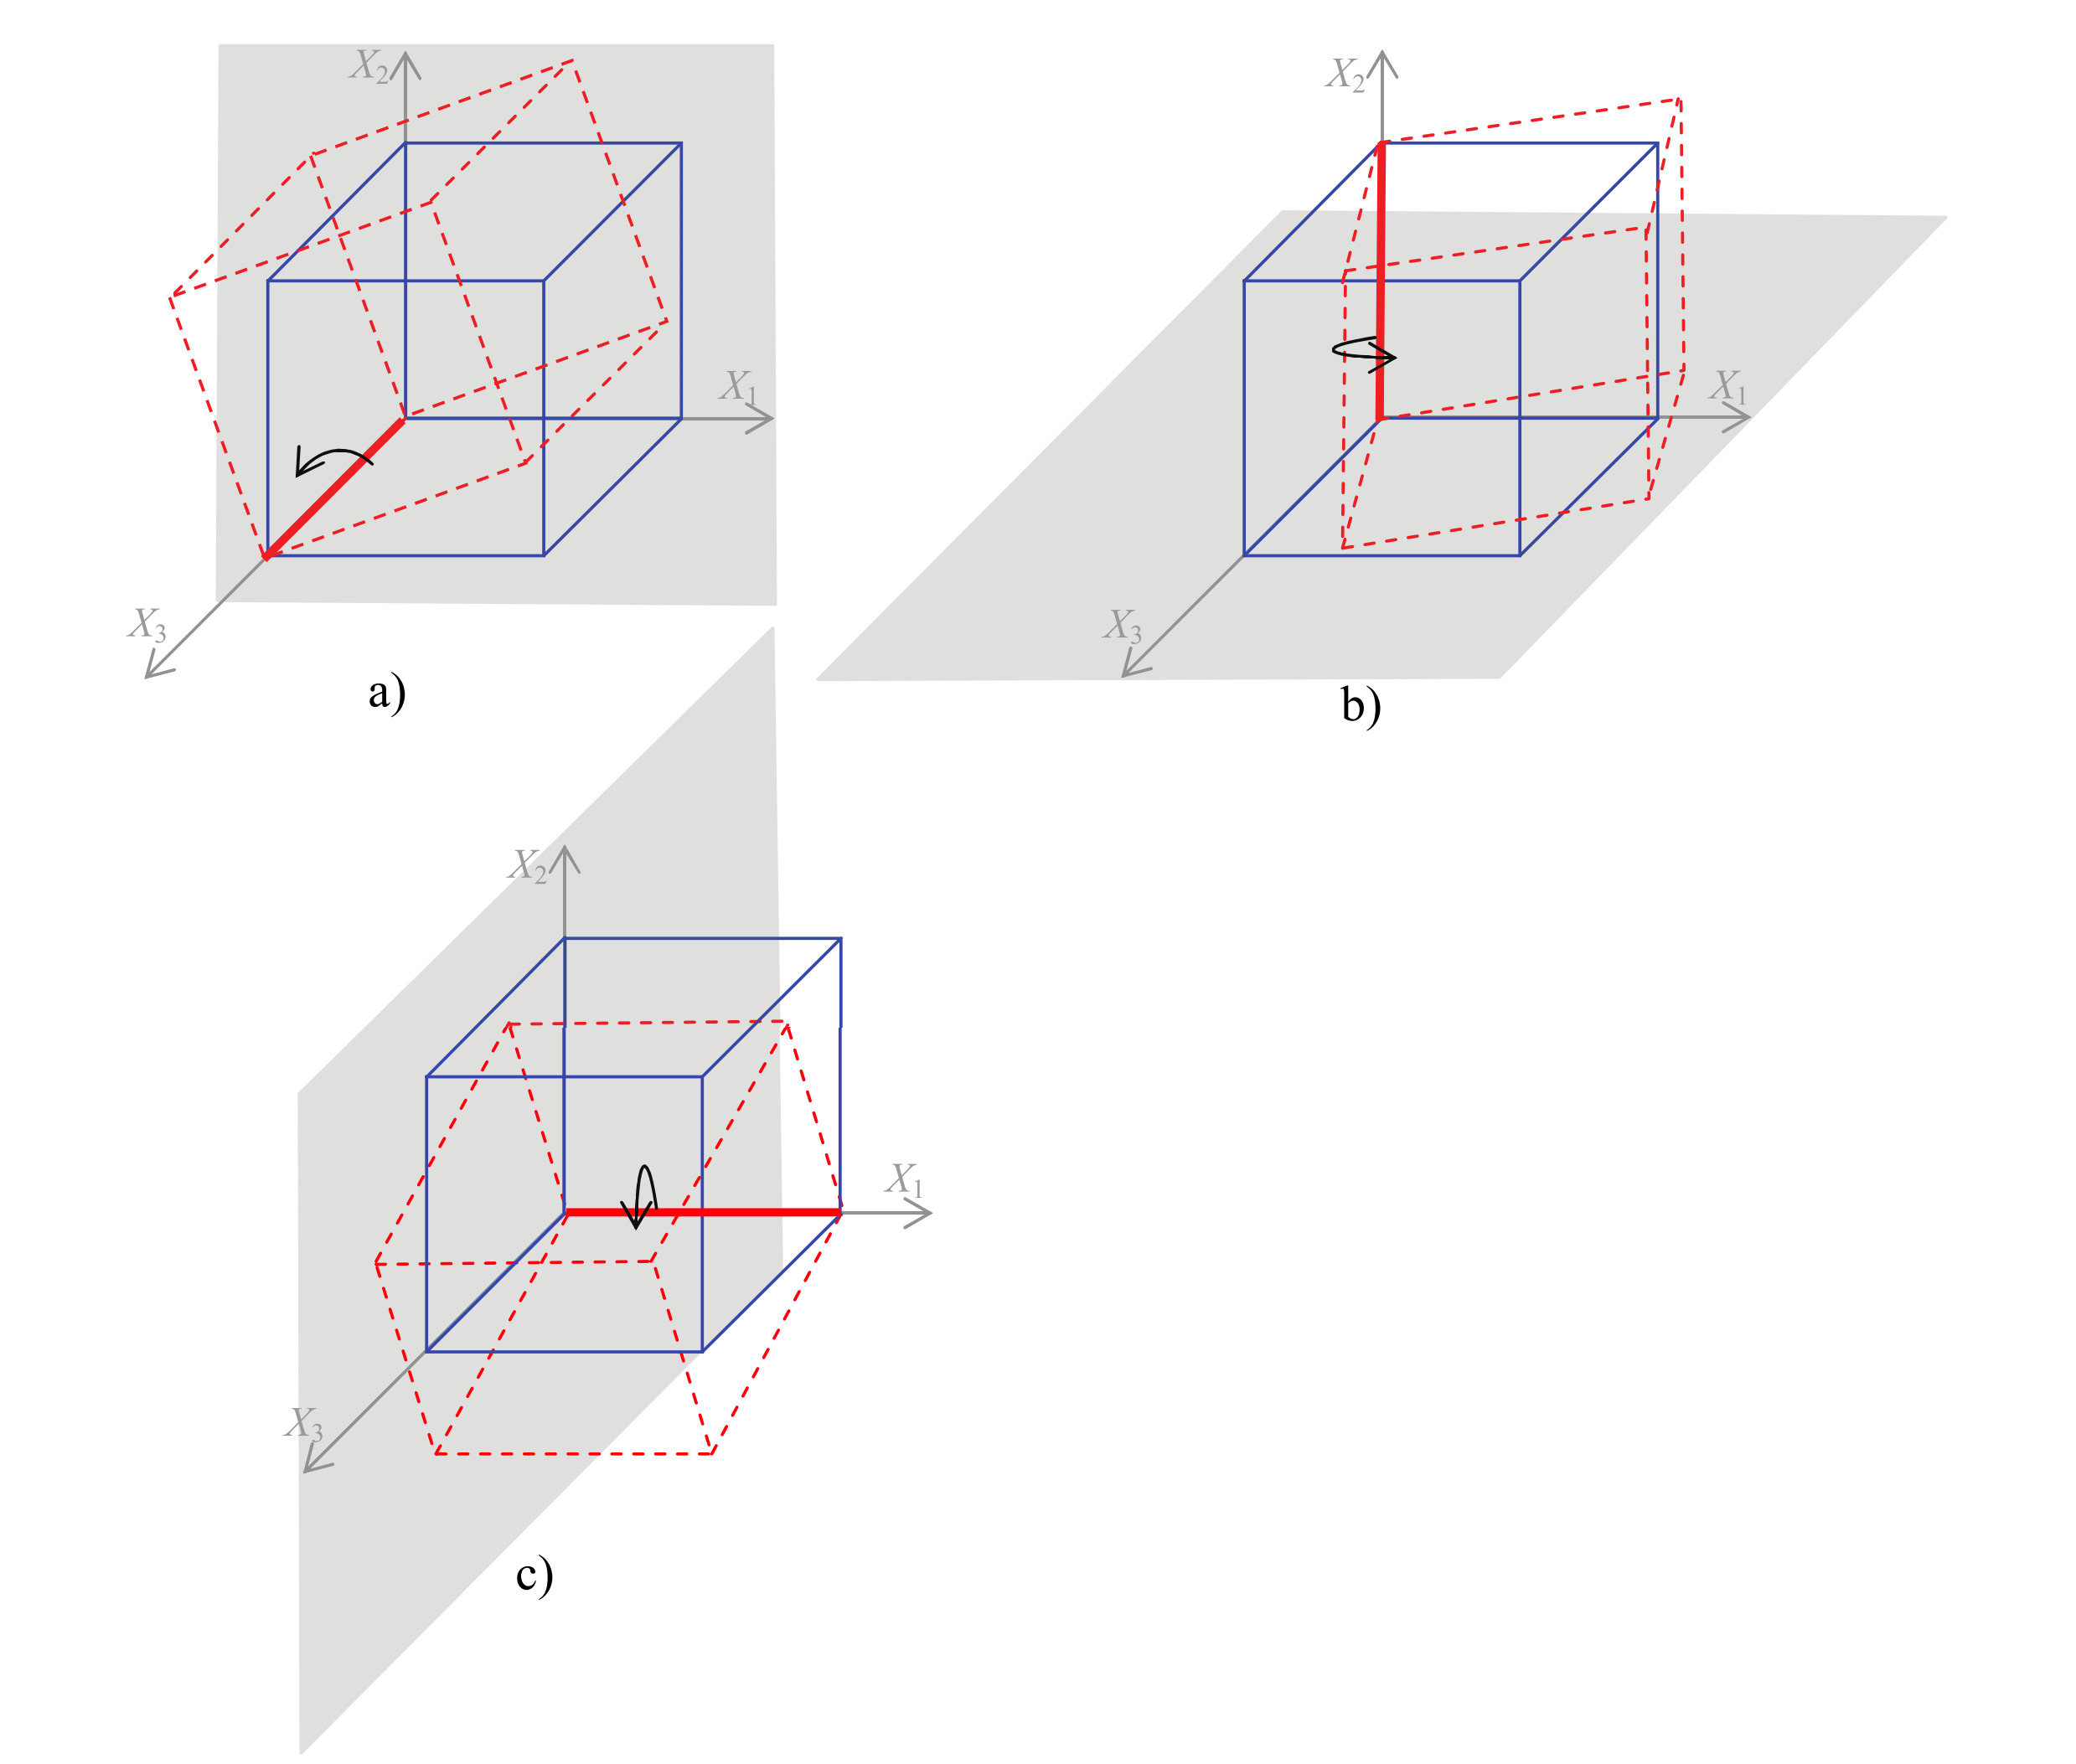
\includegraphics[width=12cm]{Img/GEO/geo-ejes.jpg}
\centering
    \caption{\footnotesize{\textbf{Rotaciones principales 3D: a) eje $X_3$, plano $X_1X_2$,   b) eje $X_2$, plano $X_1X_3$   y c) eje $X_1$, plano $X_2X_3$.}}}
    \label{rotaciones}
\end{figure}





\begin{equation}
\label{eq:rotaciones}
\footnotesize{
   \begin{cases}
   \begin{array}{rccl}
    
    R_3(\theta) = R_{1,2}(\theta)
    =
    \left[
    \begin{array}{rccl}
    \cos\theta & \sin\theta & 0 & 0\\
    -\sin\theta & \cos\theta & 0  &  0\\
    0 & 0 & 1 & 0 \\
    0 & 0 & 0 & 1\\
    \end{array}
    \right]
   
    &
    R_1(\theta) = R_{2,3}(\theta)
    =
    \left[
    \begin{array}{rccl}
    1 & 0 & 1 & 0\\
    0 & \cos\theta & \sin\theta &  0\\
    0 & -\sin\theta & \cos\theta & 0 \\
    0 & 0 & 0 & 1\\
    \end{array}
    \right]
    \\ \\
    R_2(\theta) = R_{3,1}(\theta)
    =
    \left[
    \begin{array}{rccl}
    \cos\theta & 0 & -\sin\theta & 0\\
    0 & 1 & 0 &  0\\
    \sin\theta & 0 & \cos\theta & 0 \\
    0 & 0 & 0 & 1\\
    \end{array}
    \right]
    
    \end{array}
\end{cases}
}
\end{equation}


\begin{center}
\caption{\footnotesize{\textbf{Renombramiento de las matrices de rotación 3D en términos de planos de rotación.}}}
\end{center}
    
También se cumple que las rotaciones 3D dejan fijo un subespacio uni-dimensional, 
tal subespacio es el eje de rotación, lo que significa que todos los puntos que 
caen sobre este eje, no se ven afectados por la rotación. Esto se puede ver 
gráficamente en la Figura \ref{rotaciones}, donde se observa que en cada una 
de las rotaciones, los puntos que caen sobre el eje de rotación no se ven afectados 
durante el giro. Si se renombran las matrices de rotación 3D, en términos de planos 
de rotación, colocando como subíndices los ejes que forman dicho plano se tiene la \ref{eq:rotaciones}.

Las Rotaciones principales 3D se cumple cuando el plano de rotación y el eje (n-2)-dimensional están formados por los ejes coordenados. También las \textit{Rotaciones Generales 3D} cuando el plano de rotación y el eje están definido por puntos arbitrarios y no mediante los ejes coordenados, sin embargo para los fines prácticos de este trabajo de investigación, es suficiente conocer los conceptos de las rotaciones principales.
\vskip

\subsubsection{Transformaciones Compuestas}
Con la representación matricial se puede aplicar una secuencia de transformaciones, calculando simplemente la multiplicación matricial de cada una de las matrices de transformación. Dado que se está manejando una representación de la posición de un punto p como vector renglón, se puede aplicar una transformación compuesta a un punto $p$, multiplicando las matrices de izquierda a derecha, comenzando con el punto $p$.
Por ejemplo, si se desea aplicar una translación, seguida de un escalamiento a un punto $p$, la posición final del punto $p^{\prime}$ se calcula de la siguiente manera:

$$p^{\prime} = (p. T(d)).S(s)$$
o bien una traslación seguida de una rotación:
$$p^{\prime} = (p.T(d)).R_{a,b}(\theta)$$

Las matrices de transformaciones compuestas para el caso que sean del mismo tipo, se comportan de la siguiente manera:

\begin{itemize}
  \item Las traslaciones sucesivas son aditivas: $T(d_a).T(d_b) = T(d_a + d_b)$
  \item Los escalamientos sucesivos son multiplicativos: $S(s_a).S(s_b) = S(s_a . s_b)$
  \item Las rotaciones sucesivas son aditivas: $R_{a,b}(\theta).R_{a,b}(\omega) = R_{a,b}(\theta + \omega)$
\end{itemize}

\clearpage
\subsection{Historia del Modelado Geométrico}

Las raíces del Modelado Geométrico se encuentran en los primeros sistemas gráficos, que fueron desarrollados al comienzo de la década de los 60 con propósitos CAM. Esto di lugar a la revolución industrial de la maquinaria numéricamente controlada en ingles \textit{Numeric Control} (NC)\footnote{El control numérico o control decimal numérico es un sistema de automatización de máquinas herramienta que son operadas mediante comandos programados.}.
El siguiente paso importante fue dado en el MIT\footnote{http://web.mit.edu/}, con el desarrollo de un compilador para un lenguaje de descripción gráfica en 1967. Paralelamente, las principales multinacionales en los campos automovilísticos, aviación, etc. desarrollaron sus primeros sistemas gráficos de diseño.
A mediados de los 70 se produjeron avances significativos en el Modelado Geométrico. Las limitaciones iniciales que presentaban los primeros sistemas gráficos fueron superadas desarrollando nuevas técnicas, las cuales permitieron realizar lo que conocemos como superficies esculpidas en ingles \textit{sculptured surfaces}, las superficies paramétricas, de Bezier, etc.
Mientras tanto, se desarrollaron los primeros modeladores alámbricos en inglés \textit{wireframe} y los esquemas poligonales, de los cuales hablaremos más tarde. Inicialmente estos sistemas fueron bidimensionales y trataban de implantar lo que se conoce como \textit{dibujo técnico} para ser realizado con la computadora \citep{Ramos2012}.
Finalmente surgieron los esquemas de Modelado de Sólidos (o Modelado Sólido), sobre los que se desarrolla a continuación.



\section{Modelado Sólido}
\textit{El \textbf{Modelado Sólido} es una rama relativamente reciente del Modelado Geométrico, que hace hincapié en la aplicabilidad general de los modelos, e insiste en crear solamente modelos ``completos" de los sólidos, es decir, modelos que son adecuados para responder algorítmicamente a cualquier pregunta geométrica que se formule.} \citep{Ramos2012} 

El objetivo de ``aplicabilidad general" diferencia los esquemas de Modelado Sólido de otros esquemas de modelado geométricos, los cuales se utilizan en casos especiales. Así, los modelos gráficos en inglés \textit{graphical models} se utilizan para describir el dibujo técnico de los objetos, por ejemplo en ingeniería.
Los modelos de superficie en inglés \textit{surface models} proporcionan información detallada sobre superficies, pero no siempre proporcionan la información suficiente para determinar todas las propiedades geométricas. 

\begin{figure}[h]
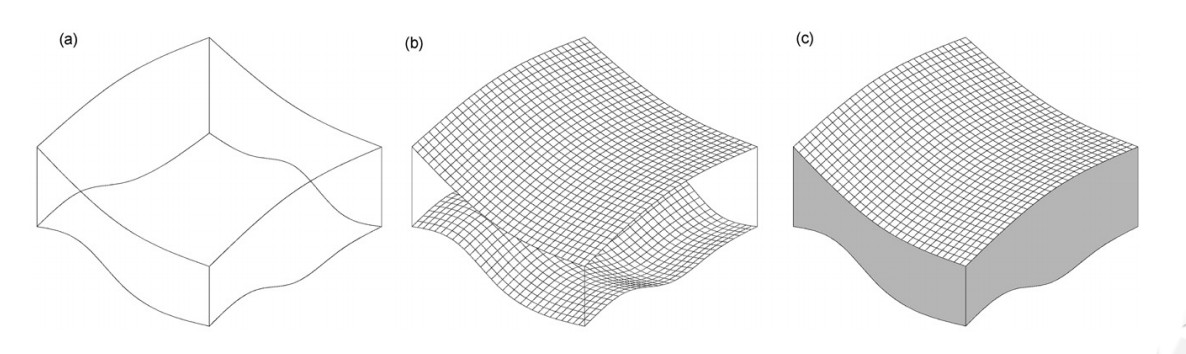
\includegraphics[width=15cm]{Img/GEO/geo-compa.jpg}
\centering
\caption{\textbf{\footnotesize{Modelos 3D: a) wireframe, b) surface, c) sólido}}}
\end{figure}


De acuerdo con el principio de universalidad, se espera de los modelos sólidos que sean capaces de responder algorítmicamente a las preguntas geométricas típicas que aparecen en las aplicaciones de ingeniería. Estos son algunos ejemplos de dichas preguntas:
¿Cuál es el aspecto del objeto? ¿Cuál es su peso, área, etc.? ¿Toca el objeto a otro
si se mueven? ¿Qué carga puede soportar? ¿Cómo puede fabricarse con los procesos de
manufacturación disponibles?\vskip
La respuesta a estas preguntas podría ser una imagen, un número o una constante booleana. De hecho, incluso podría ser otro modelo sólido,
como por ejemplo en la siguiente pregunta: ¿cuál es el efecto del proceso de fabricación aplicado a este objeto? Obviamente, es importante que un sistema de Modelado Geométrico incluya la posibilidad de modelar no sólo objetos físicos, sino también los efectos de aplicar sobre ellos procesos físicos. El sistema de modelado también debería ser capaz de realizar iteraciones, realizando operaciones sobre los resultados obtenidos al hacer operaciones similares anteriormente. Es decir, las operaciones disponibles en el sistema de modelado deben formar un sistema cerrado donde se garantice que todas las operaciones mantengan la corrección de los modelos generados en las operaciones anteriores.

Las ventajas prácticas del modelado sólido son:
\begin{itemize}
    \item Agiliza el desarrollo y los detalles del diseño.
    \item Mejora la visualización y la comunicación.
    \item Elimina los problemas de interferencias del diseño.
    \item Comprueba la funcionalidad y el rendimiento del diseño (sin la necesidad de prototipos físicos).
    \item Proporciona de forma automática las características topológicas para la fabricación digital, necesarias al programar maquinas herramienta de CNC, impresoras 3D, etc.
\end{itemize}
 


\begin{figure}[h]
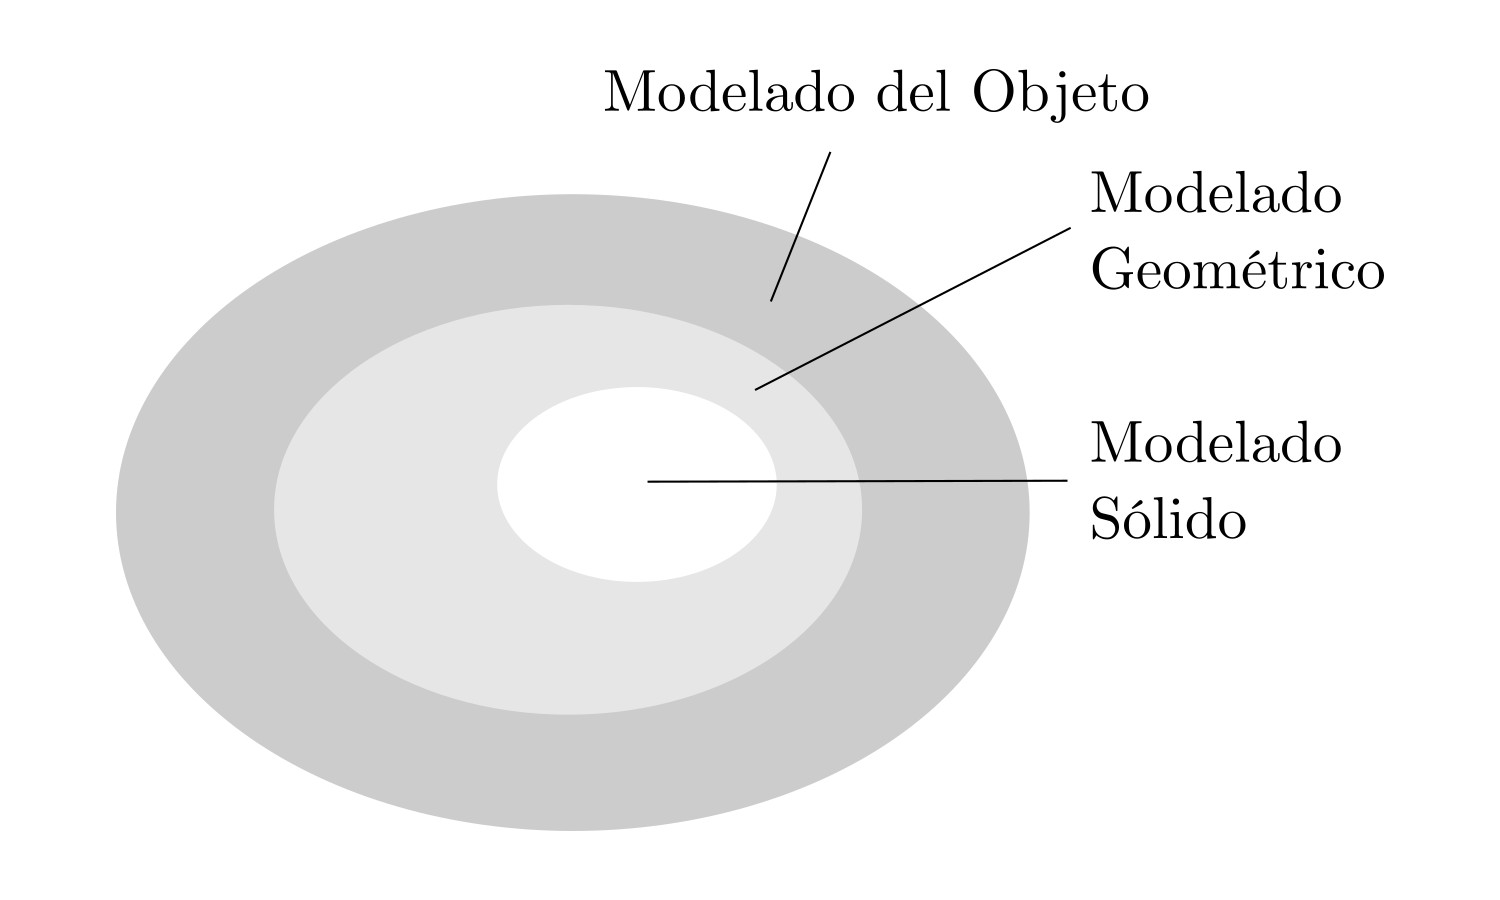
\includegraphics[width=10cm]{Img/GEO/geo-modelado0.jpg}
\centering
\caption{\textbf{\footnotesize{Estructura de subconjuntos en el Modelado}}}
\end{figure}


\subsection{ Historia del Modelado Sólido }
Las universidades de Hokkaido y Cambridge desarrollaron los primeros sistemas gráficos basados en esquemas de Modelado Sólido: TIPS y BUILD \citep{Toriya:1993:CPA:562297}, respectivamente. Se presentaron en Budapest en 1.973, demostrando su superioridad sobre cualquier otro sistema de Modelado Geométrico.
TIPS utiliza figuras básicas o primitivas\footnote{ Las formas geométricas se consideradas primitivas por su básica constitución en las partes que la conforman por ejemplo cubo, cono, esfera.} y operaciones booleanas\footnote{Las operaciones booleanas se basan en los modelos que se estudian con el álgebra de Boole, se utilizan conceptos de suma, resta, intersección, etc. para el modelado de sólidos.} para definir sólidos en tres dimensiones. Esta técnica se conoce actualmente como Geometría Constructiva de Sólidos en inglés \textit{Constructive Solid Geometry} (CSG), también llamado Modelado Booleano.
BUILD define los objetos como un conjunto de superficies, más la información topológica que las relaciona (cómo se conectan las caras, aristas y vértices). Hoy se conoce esta técnica como la Representación por Fronteras en inglés \textit{Boundary Representation} (B-Rep).
Desde entonces han surgido otros muchos modeladores, pero la gran mayoría usan conceptos de los dos anteriores o incluso de ambos (Modeladores Híbridos).
En 1977 se desarrolló en la universidad de Rochester (Estados Unidos) el sistema gráfico PADL-1 \citep{Toriya:1993:CPA:562297}, que utiliza CSG para definir los objetos, pero que puede convertir automáticamente las representaciones a B-Rep. La conversión en sentido contrario presenta muchos problemas. 

\begin{figure}[h]
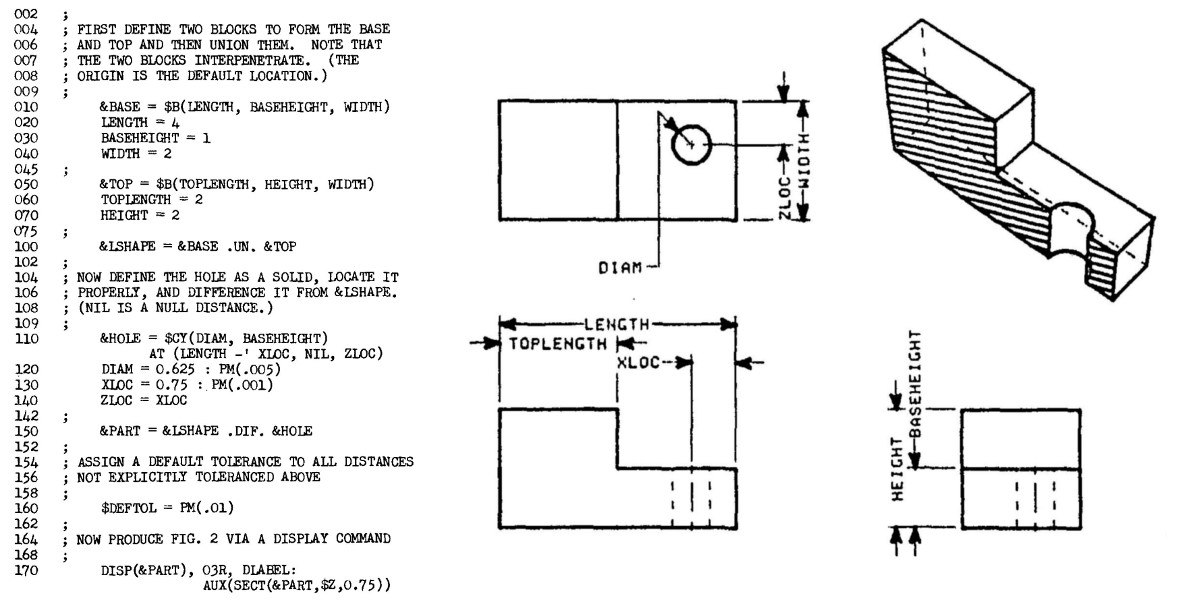
\includegraphics[width=16cm]{Img/GEO/geo-padl.jpg}
\centering
\caption{\textbf{\footnotesize{Ejemplo de modelado con PADL-1}}}
\end{figure}

\clearpage
\subsection{ Problemas del Modelado Sólido }
\label{sectionproblema}

El requerimiento de aplicabilidad general de los modelos sólidos implica la necesidad de que sean completos y exactos. Conseguir esto resulta problemático.
A continuación se explican los puntos más conflictivos: 

\subsubsection{Que sean completos}

En general, los modelos gráficos 2D no sirven para el Modelado Sólido, porque evidentemente no se puede responder algorítmicamente a todas las preguntas geométricas en tres dimensiones a partir de dibujos realizados en 2D.
Los modelos gráficos bidimensionales pueden ser transformados en modelos tridimensionales, añadiendo la información de la tercera coordenada.
De esta forma se obtiene una representación de sólidos conocida normalmente como modelo alámbrico \footnote{Los modelos alámbricos se caracterizan por no disponer de superficies, sólo consta de puntos, líneas y curvas con las que se describen los lados de los objetos.} del inglés \textit{wireframe model}. Con el modelo alámbrico es posible almacenar un solo modelo tridimensional, y generar todas las vistas bidimensionales a partir de él, superándose de esta manera los problemas planteados por los modelos gráficos en 2D.
Sin embargo, un grupo de líneas tridimensionales no es suficiente para representar una figura ya que, en ocasiones, se pueden dar varias interpretaciones.
Un ejemplo común es mostrado en la Figura \ref{fig:problema0}.

\begin{figure}[h]
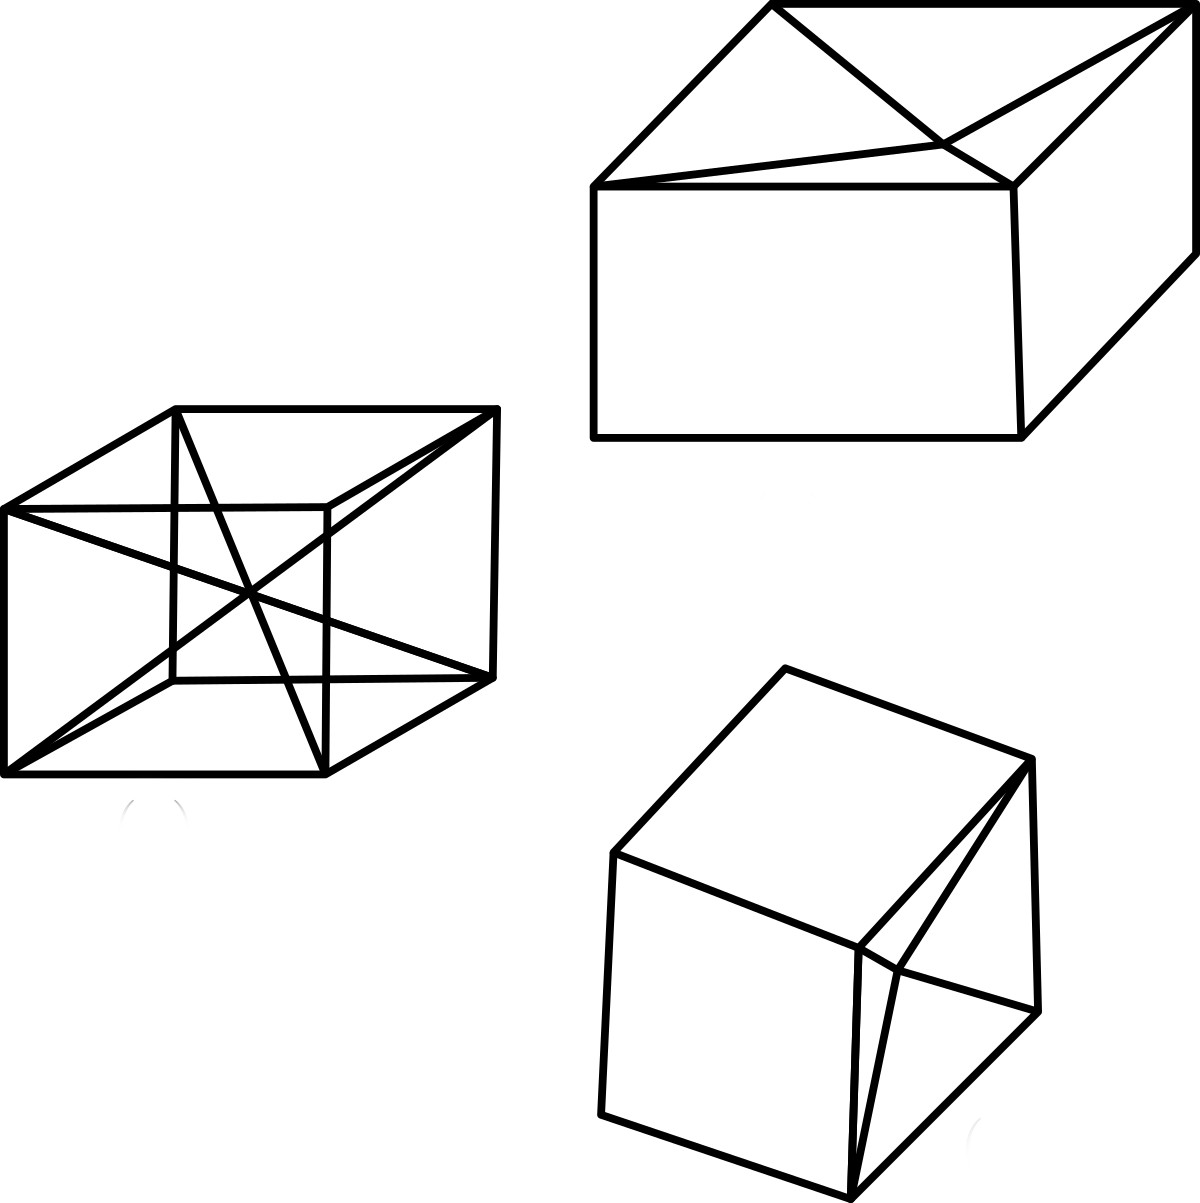
\includegraphics[width=6cm]{Img/GEO/geo-problema.jpg}
\centering
\caption{\textbf{\footnotesize{posibles interpretaciones de un modelo gráfico ambiguo. }}}
\label{fig:problema0}
\end{figure}

\vskip
Otro problema que plantean los modelos alámbricos es que permiten el diseño de objetos que no pueden ser creados como objetos 3D reales, según se muestra a continuación. 
\begin{figure}[h]

\includegraphics[width=10cm]{Img/GEO/geo-problema1.png}
\centering
\caption{\textbf{\footnotesize{posibles interpretaciones de un modelo gráfico ambiguo. }}}
\end{figure}

\vskip
Otra deficiencia de los modelos alámbricos es la falta de contorno o información de perfil para las superficies supuestas entre las aristas alámbricas.

\begin{figure}[h]

\includegraphics[width=12cm]{Img/GEO/geo-problema2.png}
\centering
\caption{\textbf{ \footnotesize{información de contorno perdida. }}}
\end{figure}



\subsubsection {Integridad}

Para resolver el problema de eliminar líneas y superficies ocultas, normalmente
se reemplazan los modelos gráficos por \textit{modelos poliédricos}\footnote{Un modelo poliédrico es un modelo geométrico cuyas caras son planas y encierran un volumen finito.} Estos modelos proporcionan la suficiente información para identificar las partes de los objetos que quedan ocultas al observador. Se construyen a partir de primitivas bidimensionales (polígonos) en vez de sólo líneas.\vskip
Al remplazar líneas por polígonos aparecen nuevos problemas. Normalmente,los algoritmos de eliminación de líneas ocultas asumen que los polígonos no intersequen entre sí, excepto en los vértices y aristas comunes.
Obviamente, un modelo poliédrico no puede incluir polígonos con intersecciones entre ellos, pues la superficie del objeto tendría intersecciones consigo misma. Por lo tanto, sólo se considerarán válidos a aquellos modelos poliédricos con polígonos sin intersecciones mutuas. Pero ¿cómo asegurarse de que los modelos cumplen este criterio?\vskip
El comprobar que el Modelado Sólido cumple este u otros requisitos preserva la \textit{integridad} del modelo, evitando la generación de modelos incorrectos.
Sin embargo, la comprobación de la integridad de los modelos trae consigo una disminución en la facilidad de uso y flexibilidad de los sistemas de modelado. 

\subsubsection{Complejidad y cobertura geométrica} El problema de la integridad está relacionado con otro: la \textit{complejidad} en la generación de un modelo poliédrico. Incluso objetos relativamente simples requieren más de cien polígonos; generar toda esa información a mano es complicado, tedioso y propenso a errores.
La \textit{cobertura geométrica} de un modelo poliédrico no es suficiente para tareas que requieren un modelado exacto de superficies curvas (como la carrocería de un coche), motivo por el cual se han desarrollado métodos para manejar formas complejas. 

\clearpage

\subsection{ Fundamentos del Modelado Sólido }
Un sistema de Modelado Sólido maneja dos tipos de información: los datos geométricos y datos topológicos. Los datos geométricos son aquellos que representan geométricamente los objetos (coordenadas de vértices, ecuaciones de superficies...). En cambio, los topológicos se refieren a cómo conectar componentes geométricos para conseguir un modelo.
A continuación se desarrollan las características topológicas más útiles en modelado (en 2 y 3D), que sirven principalmente para validar la integridad de los modelos \citep{Ramos2012} .

\subsubsection{ Teorema del camino cerrado }
El giro total a lo largo de un camino cerrado es un entero múltiplo de 360°. Este entero se conoce como número de rotaciones (\textbf{Nr}) del camino. El valor de Nr es independiente de dónde se comience el recorrido del camino y de cómo esté orientado.

\begin{figure}[h]

\includegraphics[width=8cm]{Img/GEO/geo-camino.jpg}
\centering
\caption{\textbf{\footnotesize{Ejemplo de caminos cerrados con valores de Nr diferentes.}}}
\end{figure}

\subsubsection{ Teorema del camino cerrado simple }
\textit{Un camino cerrado simple es aquél que no se corta a sí mismo}.\vskip
El teorema del camino cerrado simple dice que el giro total en un camino cerrado que no se corte a sí mismo es $\pm 360^\circ$. En otras palabras, el número de rotación Nr de un camino cerrado simple es $\pm1$.

\begin{figure}[h]
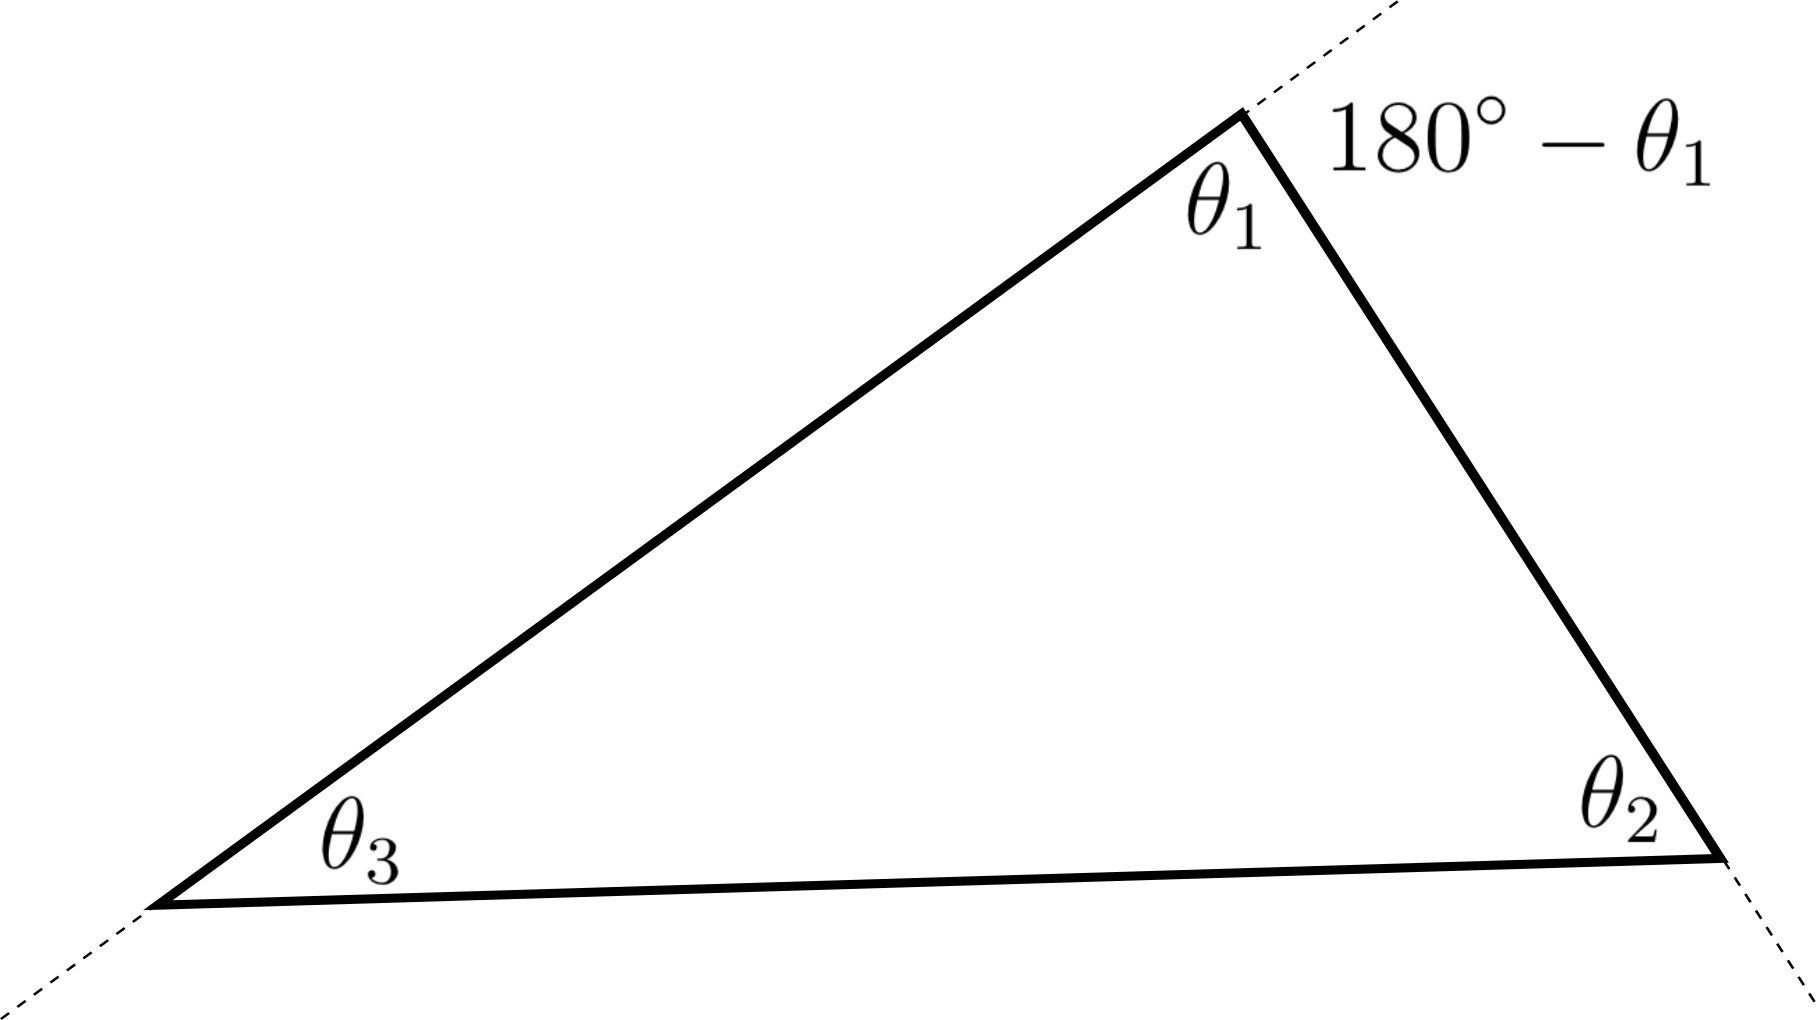
\includegraphics[width=8cm]{Img/GEO/geo-caminos.jpg}
\centering
\caption{\textbf{\footnotesize{La suma de los ángulos de giro en un camino cerrado simple es $\pm 360^\circ$}}}
\end{figure}

Por ejemplo, en el triángulo de la figura anterior, siendo $\theta_1, \theta_2$, y  $\theta_3$ sus ángulos internos, la suma de los ángulos de giro es:

\begin{equation}
(180^\circ - \theta_1) + (180^\circ - \theta_2 ) + (180^\circ - \theta_3) = 3\cdot180 - ( \theta_1 + \theta_2 + \theta_3) = 540 -180 = 360^\circ
\end{equation}

Recordemos que la suma de los ángulos interiores de un triángulo (en la geometría euclidiana) es siempre $180^\circ$.\vskip
La importancia del teorema anterior en modelado radica en que es relativamente fácil medir los giros de los camino cerrados (ej., los ángulos de los polígonos), aplicando métodos locales. De este modo, si al finalizar el recorrido de un camino cerrado (aristas de un polígono) el acumulado final del giro es diferente a $360^\circ$ podemos asegurar que el modelo no es íntegro (está mal construido), ya que uno de sus polígonos se autointerseca, como ocurre en el ejemplo de la figura 3.9.

\begin{figure}[h]

\includegraphics[width=6cm]{Img/GEO/geo-caminon.jpg}
\centering
\caption{\textbf{\footnotesize{La suma de los ángulos de giro en un camino cerrado no simple es diferente de $\pm 360^\circ$}}}
\end{figure}

\subsubsection{ Deformación de curvas y planos }

El teorema de deformación de curvas y planos dice que \textit{cualquier curva cerrada simple de un plano se puede transformar mediante una isotopía de ambiente en un cuadrado}.\vskip
En 1936, H.Whitney y W.C.Graustein observaron que dos caminos cerrados coplanarios pueden transformarse el uno en el otro sólo si tienen el mismo giro total. Este resultado junto con el teorema anterior se puede utilizar para probar el teorema del camino cerrado simple: por una parte, cualquier curva cerrada simple en un plano se puede transformar en un cuadrado, y además, un camino cerrado sólo puede transformarse en otro si tiene el mismo giro total. Entonces se puede deducir que cualquier camino cerrado simple tiene el mismo giro total que un cuadrado, es decir, $\pm 360^\circ$, con lo que se demuestra el teorema.\vskip
Las transformaciones pueden ser de dos tipos:

\begin{itemize}
\item \textit{Homotopía regular}. Es una deformación que produce cambios en el camino.
\item \textit{Isotopía de ambiente}. Suponer el camino dibujado sobre una lámina de goma. Si se estira o encoge la lámina por diferentes puntos, se puede conseguir que varíe la trayectoria del camino, o sea, una isotopía de ambiente o transformación de hoja de goma.
\end{itemize}

La homotopía regular es más drástica (no conservadora) que la isotopía de ambiente (conservadora), ya que puede crear o eliminar puntos de corte, cosa que no hace esta última. De hecho, una isotopía de ambiente es un caso especial de la homotopía regular, en la que no se añaden ni eliminan puntos de corte.


\begin{figure}[h]
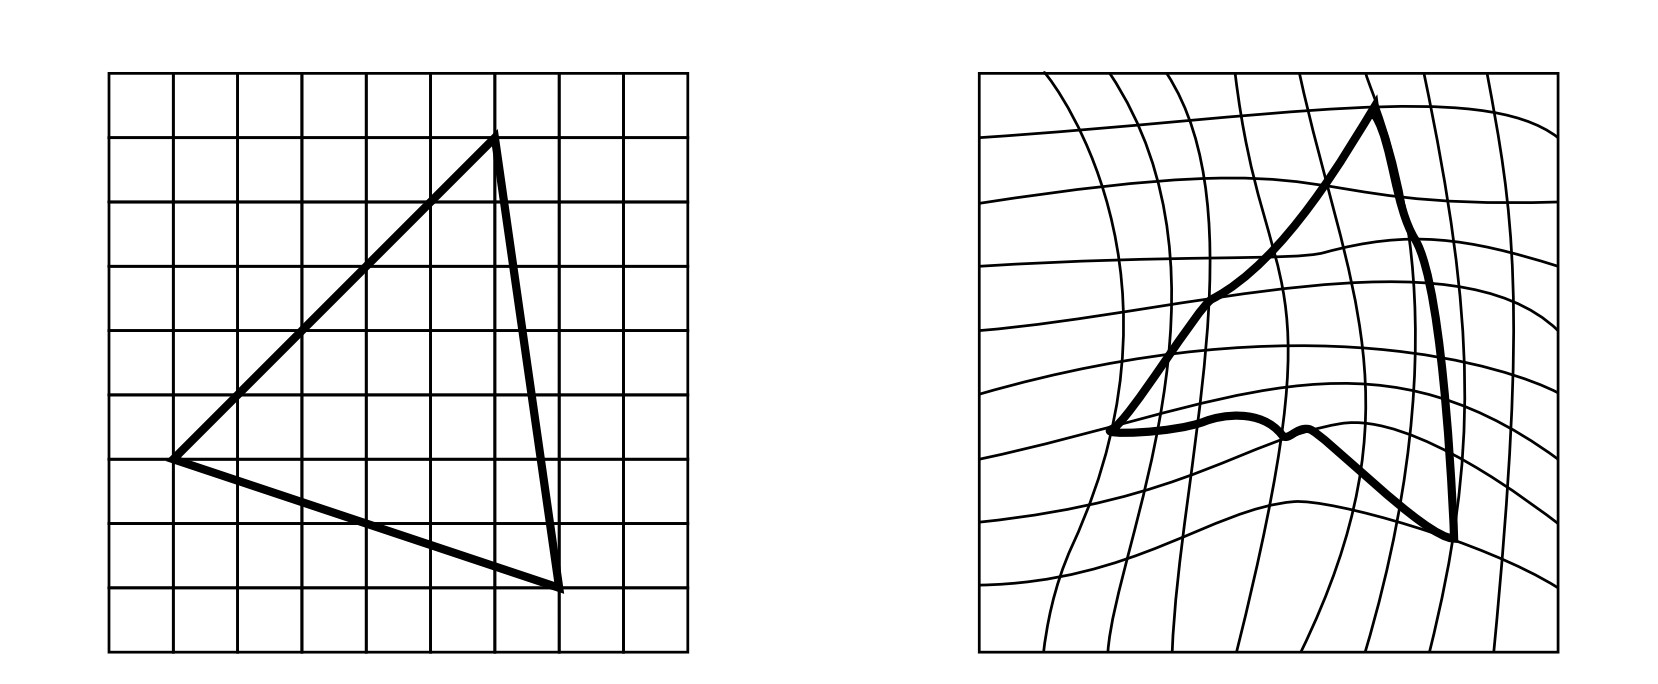
\includegraphics[width=14cm]{Img/GEO/geo-goma.jpg}
\centering
\caption{\textbf{\footnotesize{Deformación conservadora en una hoja de goma}}}
\end{figure}


\subsubsection{ Teorema de la curva de Jordan }
Se deduce del teorema de deformación de curvas y planos y dice que \textit{cualquier curva cerrada simple en un plano, divide a éste en dos regiones: una interior y otra exterior.} Da igual de qué curva cerrada simple se trate, pues siempre va a dividir al plano en una
parte interior a la curva y otra exterior. Este teorema es válido sólo para curvas que estén en superficies planas, ya que podemos trazar una curva cerrada simple en un toro, por ejemplo, y no dividirlo en dos regiones.
El interior de la curva es deformable mediante una isotopía de ambiente y puede
transformarse en un cuadrado. Una región, plana o no, que pueda ser transformada mediante una isotopía de ambiente en un cuadrado se llama \textit{disco topológico} y se caracteriza porque no tiene huecos ni puntos aislados en él.

\subsubsection{ Ángulo de Exceso }

Se conoce como ángulo de exceso (o simplemente exceso), \textit{el ángulo de giro implícito a un camino cerrado trazado sobre una superficie.} También se define como el giro que experimenta un puntero de referencia cuando es llevado alrededor de un camino cerrado. Como pronto se verá, el ángulo de exceso está íntimamente relacionado con la curvatura de las superficies.\vskip
El concepto de ángulo de exceso sirve para generalizar el teorema del camino cerrado simple, de modo que también sea válido para caminos cerrados simples sobre superficies
curvas. La generalización de este teorema nos dice que el giro total a lo largo de un camino cerrado simple, más el ángulo de exceso, debe ser igual a $360^\circ$, es decir, que:

\begin{equation}
 T+E=360   
\end{equation}

donde:

\begin{description}
\item T = Giro Total a lo largo del camino.
\item E = Ángulo de exceso a lo largo del camino.
\end{description}

Para aclarar este concepto obsérvese la figura siguiente

\begin{figure}[h]
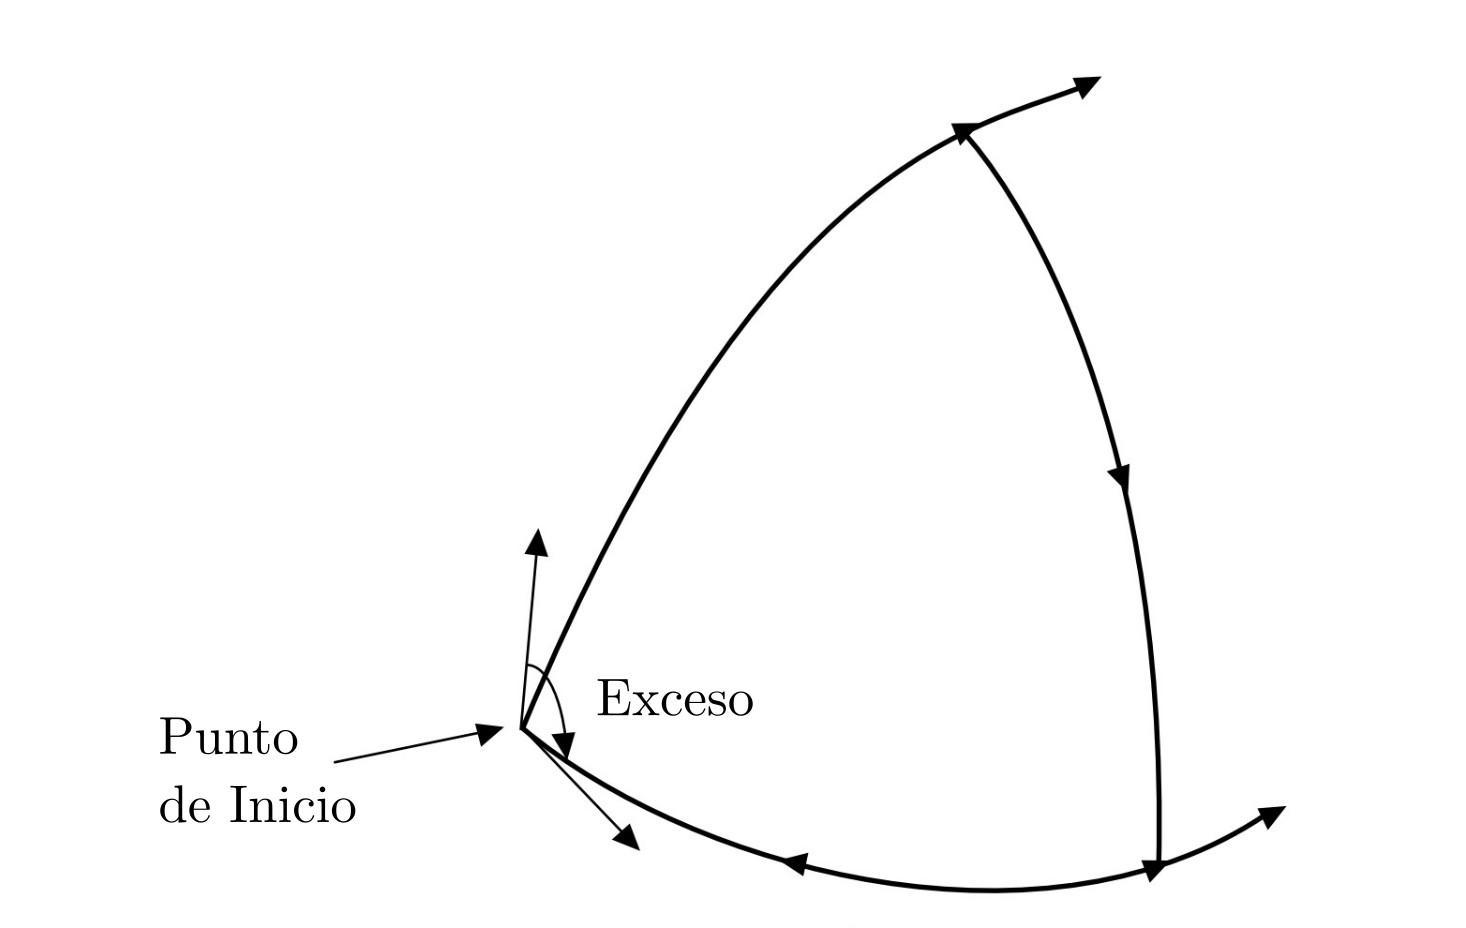
\includegraphics[width=8cm]{Img/GEO/geo-curva.jpg}
\centering
\caption{\textbf{\footnotesize{Concepto de ángulo de exceso}}}
\end{figure}

En esta figura se representa un cuadrante esférico. Supongamos que comenzamos a
andar desde el punto de inicio, con un puntero sobre nuestra cabeza apuntando hacia el polo. Al llegar a éste, giramos $90^\circ$ para volver al ecuador (obsérvese que sólo giramos nosotros, no el puntero, por lo que entre nuestra nariz y el puntero hay un ángulo de $90^\circ$).
De vuelta en el ecuador, damos otro giro de $90^\circ$ para regresar al punto de inicio (ahora
nuestra nariz y el puntero miran en direcciones opuestas). Una vez allí damos otro giro de $90^\circ$ que nos dejará en la posición inicial.
Se puede ver que el giro total que hemos realizado es de $90^\circ.3 = 270^\circ$ Luego $T = 270^\circ$. En cambio lo que ha girado el puntero (ángulo de exceso) es $E = 90^\circ$. Sumando ambas cantidades obtenemos $360^\circ$ que es lo que afirma el teorema.\vskip

\textit{Cuanto más curva es la superficie mayor es el ángulo de exceso. Si la superficie es plana, el ángulo de exceso es cero.}\vskip

\textbf{Propiedades del ángulo de exceso:} \vskip
a) Para un determinado camino, su ángulo de exceso es siempre el mismo, independientemente de donde comience el recorrido.\vskip
b) El ángulo de exceso es aditivo. Así, el exceso de cualquier polígono es igual a la suma de los excesos de los sub-polígonos en que se subdivida.



\subsubsection{ Curvatura total de las superficies }

\textit{Para cualquier disco topológico en una superficie cualquiera, el exceso que se obtiene alrededor de su frontera es igual a la curvatura total del interior.}
Como el exceso posee la propiedad aditiva, si se subdivide una superficie cualquiera en piezas o trozos poligonales, y para cada polígono se calcula el ángulo de exceso, la suma de los excesos de cada polígono se conoce como \textit{curvatura total de la superficie}, y se representa por K.
\textit{La curvatura total es una constante topológica para todas las superficies cerradas}; por ejemplo, todas las esferas tienen la misma curvatura total.
Por tanto, se puede usar el ángulo de exceso para averiguar la curvatura total de un objeto, simplemente recorriendo caminos cerrados dibujados en la superficie y calculando sus ángulos de exceso.
\vskip

\vspace{5mm}
\textbf{Evaluación de la curvatura en los modelos 3D cerrados}\vskip
Dos superficies cerradas son \textbf{topológicamente equivalentes} si es posible transformar una superficie en otra mediante \textit{transformaciones conservativas}, es decir, deformaciones que no rompan o corten la superficie. Por ejemplo, un cubo y una esfera son topológicamente equivalentes, ya que es posible (al menos mentalmente) transformar progresivamente el cubo hasta convertirlo en una esfera, y viceversa. En cambio, el toro y la esfera no lo son, ya que no es posible obtener un toro a partir de una esfera sin romper (rasgar) la superficie de ésta.
\textit{Todos los objetos cerrados que son topológicamente equivalentes poseen la misma curvatura.}


\vspace{5mm}
\textbf{A) Esferas, toros y asas}

Se puede calcular la curvatura total de los objetos de diferentes familias topológicas, a partir de la curvatura total de estos tres tipos de objetos: esferas, toros y asas.
Según vimos, el exceso de un cuadrante esférico es de $90^\circ$, o lo que es igual, su curvatura es de $\pi/2$. Como todos los cuadrantes son iguales, la curvatura total de la semiesfera es $2\pi$; por tanto, la curvatura total de la esfera será de $4\phi$ $(K = 4\pi)$.
Por otro lado, aunque no se incluya la demostración, un toro (un donut o rosquilla) tiene una curvatura total 0 $(K = 0)$, lo que no implica que el toro sea plano, sino que tiene tanta curvatura positiva como negativa.\vskip
Un toro, topológicamente hablando, puede considerarse como una esfera con un asa.
El proceso de añadir asas a las esferas no es una deformación topológica conservativa, ya que se ha de cortar la superficie de éstas, para pegar las asas. Esto implica que el objeto original y el resultante (después de añadir las asas) no son topológicamente equivalentes.
Para construir un toro a partir de una esfera se procede como sigue: primero se achatan (aplanan) dos regiones circulares en la esfera. De cada región se recorta un disco liso. A continuación se pega (o cose) un asa en los huecos dejados por los discos; el asa es un cilindro hueco (tubo) y sus aristas deben hacerse coincidir con los bordes de los discos recortados. El resultado obtenido será un toro como se muestra en la Figura \ref{fig:toro}.

\begin{figure}[h]
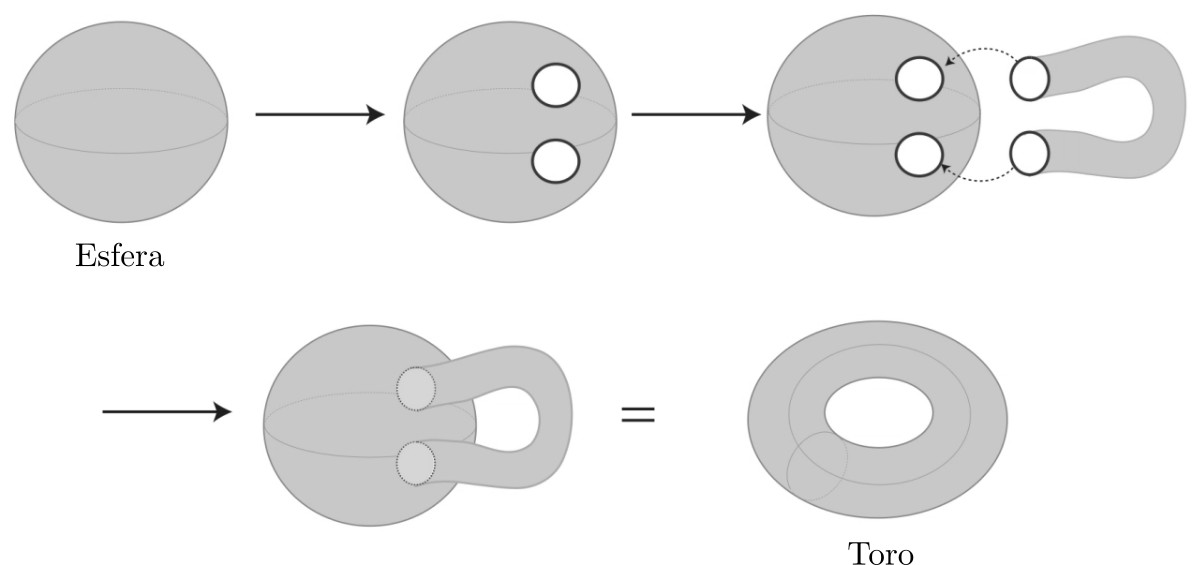
\includegraphics[width=15cm]{Img/GEO/geo-asa.jpg}
\centering
\caption{\textbf{\footnotesize{Construcción de un Toro a partir de una Esfera}}}
\label{fig:toro}
\end{figure}

En otras palabras:\vskip 
\begin{equation}
esfera - 2discos + asa = toro
\label{eq:toro}
\end{equation}
Para calcular la curvatura total del asa, en la \ref{eq:toro} se sustituyen los objetos por su curvatura correspondiente $(4\pi \ – \ 2\cdot0 + K_{asa} = 0)$ obteniéndose que la curvatura del asa es $–4\pi$. Por tanto, vemos que al añadir asas a cualquier superficie, la curvatura total de dicha superficie disminuye en $4\pi$. Además, observamos también que un toro con dos agujeros es topológicamente equivalente a un toro con un asa y a una esfera con dos asas.
En general, para una superficie topológicamente equivalente a una esfera con $g$ asas, la curvatura total es
\begin{equation}
K_{esfera \ con \ g  \ asas} = 4_{\pi}(1 - g)
\label{eq:toro1}
\end{equation}

\begin{figure}[h]
\includegraphics[width=14cm]{Img/GEO/geo-toro.jpg}
\centering
\caption{\textbf{\footnotesize{Equivalente topológico a una esfera con tres asas}}}
\label{fig:toro1}
\end{figure}

$``g”$ se conoce como \textit{orden o grado del objeto} y también como \textit{orden de la superficie}.
La importancia de esto es que cualquier superficie cerrada tridimensional que no se corte a si misma es topológicamente equivalente a una esfera con $g$ asas. Por ejemplo, una superficie como la mostrada en la Figura \ref{fig:toro1}
es topológicamente equivalente a una esfera con 3 asas.
De la \ref{eq:toro1} se deduce que \textit{la curvatura total de una superficie cerrada
en el espacio tridimensional es un múltiplo de $4\pi$}. Ver esta afirmación no
es otra cosa que la versión 3D del teorema del camino cerrado, o bien, del
teorema de camino cerrado simple si $g = 0$. Esta característica topológica de
las superficies cerradas es muy útil para la construcción y la validación de la
integridad de los modelos complicados, ya que normalmente se conoce la familia topológica $(g)$ del objeto modelado. Para ello se compara la curvatura
calculada con la indicada por la \ref{eq:toro}. Si se desconoce $g$, al menos es posible
verificar que su curvatura sea un múltiplo de $4\pi$.

\subsection{ Representación de Modelos Sólidos }

\subsubsection{ Estudio de los modelos de caras planas o poliedros }
\label{sectionpoliedro}

El estudio de los modelos de caras planas tiene una importancia especial debido a que muchos esquemas de representación usan poliedros y la topología asociada a los mismos.
Por poliedro (poli- muchos, edro- cara) entendemos una disposición de polígonos de forma que solamente dos polígonos se unen en una arista, formando el conjunto de polígonos una superficie cerrada. Además, es posible recorrer la superficie del poliedro siguiendo sus aristas.

\begin{figure}[h]
\includegraphics[width=12cm]{Img/GEO/geo-vertex.jpg}
\centering
\caption{\textbf{\footnotesize{Caras, aristas y vértices en 2 poliedros diferentes (prisma rectangular y tetraedro)}}}
\end{figure}

\vskip

\textbf{Características topológicas de los poliedros}

Conocer las características topológicas de los poliedros es importante en la construcción de los modelos y especialmente para su validación. A continuación se ven los tipos de poliedros más importantes para el modelado y sus propiedades topológicas.

\textbf{A) Poliedros simples}\vskip
Un poliedro simple es aquél que puede ser transformado de forma continua en una esfera, o sea, que es topológicamente equivalente a una esfera $(g = 0)$\vskip
Los poliedros regulares forman un subconjunto de los poliedros simples, cuya característica principal es que todas sus caras (polígonos) son iguales.
\begin{description}
\item i. Fórmula de Euler para los poliedros simples.\vskip
Para un poliedro simple se cumple que el número de vértices, menos el número de aristas, más el número de caras es 2, es decir

\begin{equation}
V - A  +  C = 2
\end{equation}

Según esta fórmula, se puede demostrar que sólo hay 5 poliedros regulares: tetraedro, hexaedro o cubo, octaedro, dodecaedro e icosaedro.
\item ii. Fórmula de Euler-Poincaré.\vskip
Poincaré generalizó la fórmula de Euler para el espacio n-dimensional. En lugar de puntos, aristas y caras, él definió elementos de $0, 1, ..., n-1$ dimensiones. A cada uno de estos elementos lo llamó, $N_0, N_1,..., N_{n}-1$, respectivamente, y expresó la fórmula de Euler como

\begin{equation}
N_0 - N_1 + N_2 - ... = 1-(-1)^n
\end{equation}

Para $n = 3$ se obtiene la fórmula de Euler. 
\end{description}


\textbf{B) Poliedros no simples. Número de conectividad y de orden}\vskip
Los \textit{poliedros no simples} son los equivalentes topológicos de cualquier objeto sólido con huecos, por lo que son muy útiles en el Modelado Sólido. En la Figura \ref{fig:polino} hay algunos ejemplos de poliedros no simples.

\begin{figure}[h]
\includegraphics[width=8cm]{Img/GEO/geo-nosimples.jpg}
\centering
\caption{\textbf{\footnotesize{ejemplos de poliedros no simples. No se pueden transformar en una esfera}}}
\label{fig:polino}
\end{figure}

Para proceder a la clasificación de los poliedros se recurre al concepto de \textbf{número de conectividad (n)}. Si la superficie de un poliedro se puede dividir en dos regiones separadas mediante un camino cerrado trazado a lo largo de sus aristas, decimos que tiene conectividad $n = 0$. Esto es así porque una esfera se puede dividir en dos partes, por cualquier camino cerrado que tracemos sobre su superficie. Se considera que la conectividad de la esfera es 0 $(n = 0)$.\vskip
De esto se obtiene un resultado: \textit{cualquier poliedro cuya conectividad sea 0 puede ser transformado en una esfera}. En la figura 13 hay caminos cerrados que no dividen a la superficie del poliedro en dos partes separadas. A estos poliedros se les asigna un número de conectividad mayor que 0.
Formalmente se define el \textit{número de conectividad como el máximo número de bucles distintos con o sin puntos comunes (intersecciones) que se puedan trazar sobre un poliedro, sin que se divida su superficie en dos regiones separadas}.
Se puede generalizar la fórmula de Euler a poliedros de cualquier número de conectividad n:

\begin{equation}
V - A + C = 2 - n
\end{equation}

Asimismo, se define el grado $``g”$ de un poliedro de la misma forma que su número de conectividad, pero sin que los bucles se intersequen. La ecuación de Euler, generalizada a poliedros de cualquier grado g es:

\begin{equation}
V - A + C = 2 - 2g
\end{equation}

de donde se deduce que $2g = n$.
Estas fórmulas son útiles porque partiendo del número de aristas, vértices y caras del poliedro, se puede saber su número de conectividad y el grado

\begin{equation*}
 n = -V + A - C + 2 
\end{equation*}

\begin{equation}
 g = \frac{(-V + A - C + 2)}{2}
\end{equation}


De este modo se sabe si los poliedros equivalen topológicamente a una esfera, a un toro, etc.

\textbf{Curvatura de los modelos poliédricos}\vskip
Toda la curvatura de las superficies de caras planas se concentra en los vértices, lo que facilita el cálculo la curvatura total \textbf{(K)}. Sólo necesitamos sumar el ángulo de exceso de los pequeños caminos alrededor de cada vértice, es decir,

\begin{equation}
K = \sum_{i=1}^{v}E_{i}
\end{equation}

donde $E_i$ es el exceso del camino alrededor del vértice $i$, y $v$ el número de vértices del poliedro.
Recordando que $T + E = 2\pi$ la ecuación anterior queda:

\begin{equation}
K = \sum_{i=1}^{v}(2\pi - T_i)
\end{equation}

donde $T_i$ es el \textit{}giro total del camino alrededor del vértice $i$. Sacando el $2\pi$ fuera del sumatorio se tiene

\begin{equation}
K = 2\pi V - \sum_{i=1}^{v}( T_i)
\end{equation}

Teniendo en cuenta que el giro total del camino alrededor del vértice \textit{$i$ $(Ti)$ es igual a la suma de todos los ángulo interiores de dicho vértice}, la expresión anterior se puede expresar más claramente si se agrupan los ángulos interiores por caras, aprovechando la propiedad asociativa de la suma.

\begin{equation}
\label{eq:poli}
K = 2\pi V - \sum_{i=1}^{C}C_i
\end{equation}

donde $ci$ es la suma de los ángulos interiores de la cara $i$ y $C$ es el total de caras del poliedro.
Este es un resultado sorprendente porque podemos calcular el segundo término sin saber cómo están unidas las distintas aristas. Por tanto, si conocemos todas las caras del poliedro y conocemos $V$, podemos calcular la curvatura total sin saber nada sobre las relaciones entre las aristas y las caras.\vskip
Para poliedros cuyas caras sean cuadrados la fórmula es todavía más simple, ya que la suma de los ángulos interiores de cualquier cara es $2\pi$.\vskip 
Por tanto, $K = 2\pi V - 2\pi C$ ó $K = 2\pi (V - C)$. Ver que esta ecuación para calcular la curvatura total no depende de los ángulos para nada.
La expresión anterior aún se puede generalizar más. Partiendo de la \ref{eq:poli}, se puede demostrar que la suma
$\sum_{i=1}^{C}C_{i}$ puede expresarse independientemente de los valores particulares de los ángulos; solamente se necesita conocer el número total de caras, vértices y aristas. Según esto, para una superficie de caras planas cerrada con $V$ vértices, $A$ aristas y $C$ caras, la \textit{curvatura total} es 

\begin{equation}
K = 2\pi (V - A + C)
\end{equation}

A la cantidad $(V - A + C)$ se le llama \textit{característica de Euler} de una superficie y se denota con la letra griega
$\chi$ (chi). Usando esta notación, rescribimos la fórmula de la curvatura como

\begin{equation}
\label{eq:chi}
K = 2\pi \chi
\end{equation}

La \ref{eq:chi} muestra que, para cualquier superficie cerrada, la curvatura total y la característica de Euler están relacionadas. Esto constituye el \textbf{teorema de Gauss-Bonnet}, y \textit{puede ser aplicado a todo tipo de superficies cerradas}, no sólo a las de caras planas, ya que la característica de Euler es una constante topológica al igual que a curvatura total. Este teorema es de suma importancia para la validación de las redes trazadas sobre superficies cerradas: \textit{todas las infinitas redes diferentes que es posible trazar sobre una superficie cerrada poseen la misma característica de Euler}.
Este teorema proporciona resultados muy importantes, ya que además de ser un medio muy útil para poder calcular la curvatura total de las superficies cerradas, da una relación entre una cantidad definida en términos topológicos, como es la característica de Euler, con otra definida en términos geométricos, como es la curvatura total.

\vspace{5mm}
\textbf{Representación topológica de los poliedros.}\vskip
Uno de los puntos clave en el modelado con poliedros es cómo se ha de registrar su información topológica, es decir, las relaciones entre los vértices, aristas y caras que los definen.
La forma más simple y directa para representar los poliedros consiste en describir cada cara por separado, señalando explícitamente cómo han de unirse. Este método de representación se conoce como \textbf{atlas}. La Figura \ref{fig:atlascubo} muestra el atlas de un cubo.

\begin{figure}[h]
\includegraphics[width=8cm]{Img/GEO/geo-atlas0.jpg}
\centering
\caption{\textbf{\footnotesize{atlas de un cubo}}}
\label{fig:atlascubo}
\end{figure}

Cada eje se etiqueta con un par de números indicando la cara y el número de la arista de la cara. Así el par (1,0) se interpreta como la arista 0 de la cara 1. Cada unión de dos aristas se especificará por dos pares de números, identificando las aristas que se unen. De esta forma, el atlas formado queda como siguiente:


$$
\begin{array}{c@{}c@{}c@{}c}
 \begin{array}{cc}
         [(1,0) & (2,0)]
  \end{array} & \begin{array}{cc}
         [(1,1) & (5,0)]
  \end{array} & \begin{array}{cc}
         [(1,2) & (4,0)]
  \end{array} &
  \begin{array}{cc}
         [(1,3) & (3,0)] 
  \end{array}
  \\
  \begin{array}{cc}
         [(2,1) & (3,3)]
  \end{array} & \begin{array}{cc}
         [(2,3) & (6,2)]
  \end{array} & \begin{array}{cc}
         [(2,3) & (5,1)] 
  \end{array} &
  \begin{array}{cc}
         [(3,1) & (4,3)]
  \end{array}
  \\
  \begin{array}{cc}
         [(3,2) & (6,3)]
  \end{array} & \begin{array}{cc}
         [(4,1) & (5,3)]
  \end{array} & \begin{array}{cc}
         [(4,2) & (6,0)] 
  \end{array} &
  \begin{array}{cc}
         [(5,2) & (6,1)] 
  \end{array}
\end{array}
$$   

\begin{center}
\textbf{\footnotesize{representación matricial del atlas}}
\end{center}

Además de especificar qué aristas están unidas, se ha de decir cómo unirlas. La Figura \ref{fig:atlas0} muestra dos formas diferentes de unir un par de aristas. La primera, mostrada a la izquierda, es la unión con \textit{orientación conservadora}, y la segunda tiene \textit{orientación inversora}. Para unir esas dos aristas hay que hacer coincidir los números de cada una de ellas. Si se hace mediante la orientación conservadora se obtiene un cilindro y una \textit{cinta de Moebius\footnote{La cinta de Möbius o Moebius es una superficie con una sola cara y un solo borde. Tiene la propiedad matemática de ser un objeto no orientable.}} con la orientación inversora.

\begin{figure}[h]
\includegraphics[width=8cm]{Img/GEO/geo-atlas1.jpg}
\centering
\caption{\textbf{\footnotesize{orientaciones conservadora e inversora}}}
\label{fig:atlas0}
\end{figure}

Para especificar en el atlas de qué forma se van a unir las aristas, utilizamos la \textit{paridad de transición} que es $\pm 1$, unida al par de aristas. La Figura \ref{fig:atlas1} presenta varios ejemplos de un esquema de notación que incluye el número de paridad de transición

\begin{figure}[h]
\includegraphics[width=11cm]{Img/GEO/geo-atlas2.jpg}
\centering
\caption{\textbf{\footnotesize{atlas y paridad de transición de una esfera, un toro y una botella de Klein.}}}
\label{fig:atlas1}
\end{figure}


\textbf{A) Superficies Orientables y No Orientables} \vskip
Si utilizamos uniones no conservadoras en un atlas podemos conseguir algunas curiosidades matemáticas llamadas \textit{superficies no orientables}, como la \textit{cinta de Moebius} y la \textit{botella de Klein}\footnote{En topología, una botella de Klein es una superficie no orientable abierta cuya característica de Euler es igual a 0 ; no tiene interior ni exterior.} (ver Figura \ref{fig:atlas2}). La cinta de Moebius posee una curiosa particularidad. Si se recorre la cinta comenzando en un punto cualquiera, y se da una vuelta completa, como se trata de una cinta bidimensional, cuando se llegue al punto de partida se observará que la derecha e izquierda están intercambiadas. Este tipo de superficies se llaman \textbf{no orientables} y se producen al efectuar uniones no conservadoras entre sus aristas. Por el contrario, si en la superficie nunca se intercambian la izquierda y derecha, entonces se dice que la superficie es \textbf{orientable}.

\begin{figure}[h]
\includegraphics[width=14cm]{Img/GEO/geo-mobius.jpg}
\centering
\caption{\textbf{\footnotesize{Cinta de Moebius y Botella de Klein}}}
\label{fig:atlas2}
\end{figure}

Habíamos visto que para que cualquier superficie cerrada tridimensional sea consistente, debe ser topológicamente equivalente a una esfera con $g$ asas. Ahora se añade otra condición más: \textit{debe ser orientable}.
Si partimos de una cinta de Moebius y la cerramos aplicando una orientación conservadora, obtenemos otra superficie no orientable llamada botella de Klein, que no se puede construir en un espacio tridimensional sin que se auto interseque.


\subsubsection{ Objetos de Euler }
A los objetos cerrados tridimensionales de orden $g \geq 0 $ que verifican ciertos
requisitos de construcción, se les denomina objetos de Euler. Dichas normas son:

\begin{itemize}
\item Todas sus caras (curvas o planas) han de ser discos topológicos. 
\item Cada arista une sólo dos caras y todas finalizan en un vértice en
cada extremo.
\item Por lo menos tres aristas se unen en un vértice. 
\end{itemize}

En los objetos de Euler se cumple que:


\begin{equation}
V - A + C  = 2(S-P)
\end{equation}

\begin{description}
\item $S$: número de superficies inconexas del objeto.
\item $P$: total de pasajes (túneles) en el objeto.
\end{description}

Como el número de pasajes en un objeto es igual al total de ``asas” o agujeros que posea, ocurre que en la ecuación anterior $P$ es igual al orden del objeto $(P = g)$.\vskip
Para entender mejor el significado de $S$, la figura \ref{fig:euler} muestra tres objetos eulerianos, con una, dos y tres superficies inconexas.

\begin{figure}[h]
\includegraphics[width=12cm]{Img/GEO/geo-euler0.jpg}
\centering
\caption{\textbf{\footnotesize{Objetos de Euler con diferentes valores de $S$}}}
\label{fig:euler}
\end{figure}

En la Figura \ref{fig:euler1} se pueden ver algunos ejemplos de objetos eulerianos, cuando $S = 1$ y $P = 0$. Ver que en este caso la Ec. 16 se reduce a la ecuación de Euler.

\begin{figure}[h]
\includegraphics[width=14cm]{Img/GEO/geo-euler1.jpg}
\centering
\caption{\textbf{{Ejemplos de objetos de Euler}}}
\label{fig:euler1}
\end{figure}


En la Figura \ref{fig:euler2} hay otros dos objetos de Euler. El izquierdo es de grado 1, ya que tiene un túnel que lo cruza; el otro, aunque posee una cavidad, ésta no llega a atravesar el modelo. Por tanto, se trata de un objeto topológicamente equivalente a una esfera, es decir, de grado 0.

\begin{figure}[h]
\includegraphics[width=8cm]{Img/GEO/geo-euler2.jpg}
\centering
\caption{\textbf{\footnotesize{Objetos eulerianos de grado 1 y 0, respectivamente}}}
\label{fig:euler2}
\end{figure}


\textbf{ Operadores de Euler.}\vskip
Los \textbf{operadores de Euler} \textit{permiten crear y transformar objetos de Euler, en nuevos objetos (también eulerianos)} mediante la adición o eliminación de caras, aristas y vértices. Dichos operadores son especialmente útiles en la creación y transformación de los modelos poliédricos, ya que directamente generan modelos íntegros, lo que evita (o minimiza) la verificación de la integridad de los modelos. Los operadores de Euler trabajan directamente sobre las estructuras de datos que definen los objetos. Por lo tanto, \textit{un operador de Euler es un proceso} que actúa sobre la base de datos donde está la información de los poliedros que ha de crear o transformar.\vskip
Durante la transformación de un objeto de Euler en otro objeto de Euler, \textit{inevitablemente se producen objetos intermedios que no son de Euler}. Por ejemplo, en la Figura \ref{fig:euler3} se pueden ver tres transformaciones realizadas con operadores de Euler. En el primer y segundo caso se han añadido las aristas y vértices suficientes para que los objetos resultantes sigan siendo de Euler. En el caso tercero, aunque cumple la ecuación de Euler, sin embargo, las aristas $(1,5)$ y $(2,5)$ no unen dos caras y, además, del vértice 5 no parten tres aristas, por lo que se trata de un objeto intermedio no euleriano. Éste puede convertirse en euleriano añadiendo dos nuevas aristas, la $(4,5)$ y la $(3,5)$.

\begin{figure}[h]
\includegraphics[width=12cm]{Img/GEO/geo-euler3.jpg}
\centering
\caption{\textbf{\footnotesize{Operaciones de Euler sobre un cubo.}}}
\label{fig:euler3}
\end{figure}

A base de añadir o eliminar aristas, vértices y caras, los operadores de Euler sólo pueden transformar los objetos de Euler en otros de la misma familia topológica. Si a partir de un objeto de grado g se pretende obtener otro de grado diferente, entonces no queda más remedio que agujerear alguna superficie (acordarse del proceso de pegado de asas) para poder construir un nuevo pasaje.\vskip
Por lo tanto, para poder cambiar el grado de los objetos, \textit{los operadores de Euler incorporan la posibilidad de añadir o eliminar agujeros a los discos topológicos que configuran los objetos de Euler}. Al agregar un agujero en una cara, se crea un objeto intermedio3 donde se cumple que:

\begin{equation}
\label{fig:ecuacioneuler}
V - A + C - O  = 2(S-P)
\end{equation}

$``O”$ es el total de orificios (agujeros) en las caras. Ver que la ecuación de los objetos eulerianos es un caso particular de ésta, ya que entonces $O = 0$.\vskip
Los sumandos de la izquierda en la expresión $V - A + C  = 2(S-P)$ pueden ser modificados directamente en la estructura de datos, mientras que los de la derecha (S y P) no. Esto significa que si, por ejemplo, se desea transformar un objeto de Euler de modo que el objeto final resultante haya cambiado de familia topológica (variado $g$), es posible conseguirlo añadiendo o eliminando vértices, aristas, caras y/o agujeros en las caras, de forma que al final se cumpla que
$V^\prime - A^\prime + C^\prime - O^\prime  = 2(S^\prime-P^\prime)$

En el ejemplo de la Figura \ref{fig:euler4}, se aprecia un objeto no euleriano con un agujero en una cara y su transformación en uno de Euler. Observar que el hecho de hacer agujeros en las caras, no implica necesariamente que el objeto euleriano resultante sea de grado diferente al del objeto original.

\begin{figure}[h]
\includegraphics[width=12cm]{Img/GEO/geo-euler4.jpg}
\centering
\caption{\textbf{\footnotesize{Transformación de un objeto no euleriano en otro de Euler.}}}
\label{fig:euler4}
\end{figure}

\textbf{A) Elección de los operadores de Euler}\vskip

Dado que interesa que los operadores de Euler sean capaces de cambiar el grado de los objetos, se utiliza la \ref{fig:ecuacioneuler} para establecer los criterios de elección de los operadores de Euler.\vskip
Se ha demostrado que \textit{no existe un conjunto de operadores de Euler que garantice la coherencia de los objetos intermedios}, es decir, que siempre se crearán objetos intermedios no eulerianos. Sin embargo, algunos operadores generan objetos intermedios más incoherentes que otros. Este hecho sirve como criterio de elección de los operadores de Euler. Así, \textit{los operadores preferidos serán aquellos que generen objetos intermedios poco incoherentes}, es decir, que se desvíen lo mínimo posible de los objetos de Euler.
Braid, Hillyard y Stroud establecieron en 1978 un conjunto de 5 operadores básicos, con los cuales es posible efectuar cualquier transformación admisible. Estos operadores son:
\begin{list_type}  
\item - PAV. Poner una arista y un vértice. 
\item - PCA. Poner una cara y una arista.
\item - PSCV. Poner una superficie, una cara y un vértice.
\item - PPS. Poner un pasaje y una superficie.
\item - PA-EO. Poner una arista y eliminar un agujero (orificio).
\end{list_type}

Estos operadores tienen otros 5 operadores complementarios, que en vez de añadir, eliminan elementos. Son:
\begin{list_type}  
\item - EAV. Eliminar una arista y un vértice. 
\item - ECA. Eliminar una cara y una arista.
\item - ESCV. Eliminar una superficie, una cara y un vértice.
\item - EPS. Eliminar un pasaje y una superficie.
\item - EA-PO. Eliminar una arista y poner un agujero (orificio).
\end{list_type}

Los operadores anteriores poseen la propiedad de mantener balanceada la \ref{fig:ecuacioneuler}, es decir, la adición o eliminación de uno o varios elementos a un lado de la ecuación queda contrarrestada añadiendo o quitando los elementos necesarios en el otro lado. Por ejemplo, el operador $PSCV$ añade un vértice (+1) y una cara (+1) en el lado izquierdo de la \ref{fig:ecuacioneuler}, y esto lo contrarresta añadiendo una superficie, que está en el otro lado de la ecuación, y tiene peso 2. Por lo tanto, como se añaden 2 por la izquierda y otros dos por la derecha, la \ref{fig:ecuacioneuler} permanece balanceada.

\begin{center}
 \begin{tabular}{ c |c c c c c c} 
   \empty & V & A & C & O & 2S & 2P \\ 
   PAV & 1 & 1 & 0 & 0 & 0 & 0 \\
   \hline
   PCA & 0 & -1 & 1 & 0 & 0 & 0 \\
   PSCV & 1 & 0 & 1 & 0 & 1 & 0 \\
   PPS & 0 & 0 & 0 & 0 & 1 & 1 \\
   PA-EO & 1 & 0 & -1 & 0 & 0 & 0 \\
   \hline
   EAV & -1 & -1 & 0 & 0 & 0 & 0 \\
   ECA & 0 & -1 & -1 & 0 & 0 & 0 \\
   ESCV & -1 & 0 & -1 & 0 & -1 & 0 \\
   EPS & 0 & 0 & 0 & 0 & -1 & -1 \\
   EA-PO & 0 & -1 & 0 & 1 & 0 & 0 \\
\end{tabular}
\end{center}
\vskip
\begin{center}
\caption{tabla 2: balance de los diferentes operadores de Euler}
\end{center}

De igual modo, el operador $PCA$ añade una cara (+1), que se contrarresta añadiendo una arista que, aunque está en el mismo lado de la ecuación, tiene signo opuesto (-1). En la tabla 2 se muestra el balanceado con respecto a la \ref{fig:ecuacioneuler}, de cada uno de los operadores de Euler vistos.\vskip
Veamos un ejemplo sobre una de las posibles secuencias de operadores de Euler para construir un tetraedro. Siendo V = 4, A = 6, C = 4, O = P = 0, y S = 1, la siguiente secuencia de operadores finaliza con la creación de un tetraedro:

\begin{center}
 \begin{tabular}{ c |c c c c c c} 
   \empty & V & -A & +C & -O & 2S & -2P \\ 
   \hline
   PSCV & 1 & 0 & 1 & 0 & 1 & 0 \\
   \hline
   PAV & 1 & 1 & 0 & 0 & 0 & 0 \\
   PAV & 1 & 1 & 0 & 0 & 0 & 0 \\
   PAV & 1 & 1 & 0 & 0 & 0 & 0 \\
   \hline
   PCA & 0 & 1 & 1 & 0 & 0 & 0 \\
   PCA & 0 & 1 & 1 & 0 & 0 & 0 \\
   PCA & 0 & 1 & 1 & 0 & 0 & 0 \\
\end{tabular}
\end{center}
\vskip
\begin{center}
\caption{secuencia de operadores de Euler para crear un tetraedro}
\end{center}

Cada uno de los procesos anteriores queda reflejado en la siguiente figura:
\begin{figure}[h]
\includegraphics[width=12cm]{Img/GEO/geo-euler5.jpg}
\centering
\caption{\textbf{\footnotesize{Construcción de un tetraedro mediante los operadores de Euler.}}}
\end{figure}

Vemos en el ejemplo que la fórmula de Euler está equilibrada en todo momento, aunque no se obtiene un sólido válido hasta después de haber realizado la última operación. El primer operador (el PSCV) se encarga de inicializar la estructura de datos, y añade un vértice, una cara e incrementa el contador de superficies. Como argumentos requiere las coordenadas del vértice y los parámetros que describen la cara (no sus aristas).

\subsubsection{ Concepto de Frontera. }

Si se tiene una región n-dimensional $R^n$ en un espacio n-dimensional $E^n$, sus puntos pueden ser clasificados como: los que están dentro de la región y
los que están en su límite o frontera. Por lo tanto, el conjunto de puntos de $R^n$ estará formado por el subconjunto de puntos interior $(iR)$, más el conjunto de los puntos de la frontera $(fR)$.

\begin{equation}
R = [iR, fR]
\end{equation}

Según lo anterior, cualquier punto en el espacio $E^n$, tiene la siguiente propiedad respecto a $R^n$:

\begin{itemize}
\item Pertenecer al interior de $R^n$, es decir a $iR$. 
\item Pertenecer a la frontera de $R^n$, es decir a $fR$.
\item No pertenecer a $R^n$. 
\end{itemize}


\begin{figure}[h]
\includegraphics[width=8cm]{Img/GEO/geo-frontera0.jpg}
\centering
\caption{\textbf{\footnotesize{objetos planos con sus puntos frontera e interiores.}}}
\end{figure}

\subsubsection{ Operadores Booleanos. }

Los objetos geométricos pueden considerarse como conjuntos de puntos, tanto de interior como de frontera. En Modelado Sólido, para construir objetos complejos se utilizan operaciones entre conjuntos, tales como unión $(\cup)$, intersección $(\cap)$ y diferencia $(−)$. A estos operadores se les conoce en modelado como \textbf{operadores Booleanos}. Al aplicar los operadores booleanos sobre objetos simples para formar modelos más complejos, es importante que los modelos obtenidos sean íntegros (topológicamente válidos), y que además sean \textit{dimensionalmente homogéneos}, es decir, que su dimensión sea igual a la de los objetos que se combinan. La Figura \ref{fig:booleano0} muestra dos ejemplos donde se pierde la homogeneidad dimensional, después de efectuar la intersección entre objetos válidos de 2 y 3 dimensiones.


\begin{figure}[h]
\includegraphics[width=14cm]{Img/GEO/geo-booleano0.jpg}
\centering
\caption{\textbf{\footnotesize{Intersección que presenta un resultado degenerado.}}}
\label{fig:booleano0}
\end{figure}

lndependientemente de cómo se presenten los objetos, es necesario combinarlos para formar nuevos. Uno de los métodos más intuitivos y comunes para combinar objetos son las \textit{operaciones booleanas de conjuntos}, como la unión, la diferencia y la intersección, ilustradas en la figura \ref{fig:booleano1}.

\begin{figure}[h]
\includegraphics[width=14cm]{Img/GEO/geo-booleano1.jpg}
\centering
\caption{\textbf{Figura 3.11. \footnotesize{Operaciones booleanas Objetos $A \ y  \ B$, $A \cup B$, $A \cap B$, $A - B$, $B - A$}}}
\label{fig:booleano1}
\end{figure}


\vspace{5mm}
\textbf{ Operadores booleanos regularizados }

La aplicación de una operación booleana ordinaria de conjuntos a dos objetos sólidos no necesariamente produce un objeto sólido. Por ejemplo, la intersección ordinaria de dos cubos que se unen en un solo vértice es un punto.\vskip
Para evitar los resultados degenerados se utiliza el conjunto de los \textbf{operadores regularizados}, que preservan la homogeneidad dimensional. Los operadores regularizados se denotan por $\cup^*$, $\cap^*$ y $-^*$ y se definen de manera que las operaciones con sólidos siempre generen sólidos.

\textbf{ A) Intersección Regularizada ($\cap^{*}$)}

\begin{figure}[h]
\includegraphics[width=12cm]{Img/GEO/geo-booleano2.jpg}
\centering
\caption{\textbf{\footnotesize{Intersección no regularizada ($\cap$) y regularizada ($\cap^*$) de dos solidos.}}}
\end{figure}

Para comprender el proceso de regularización se analizan los objetos bidimensionales A y B de la Figura \ref{fig:booleano2}, si realizamos la intersección no regularizada $(\cap)$ con dichos objetos, se obtiene un objeto que no es dimensionalmente homogéneo en su totalidad, pues contiene una ``arista colgante". El resultado deseado se obtiene mediante la intersección regularizada $(\cap^*)$ de A y B.


\begin{figure}[h]
\includegraphics[width=12cm]{Img/GEO/geo-booleano3.jpg}
\centering
\caption{\textbf{ \footnotesize{operador booleano de intersección no regularizado $(\cap)$ y el regularizado $(\cap^*)$.}}}
\label{fig:booleano2}
\end{figure}




Los objetos A y B se pueden representar como la unión de los subconjuntos de frontera e interior. Así:

\begin{equation}
   A = iA \cup fA \ \ \text{y} \ \ B = iB \cup fB
\end{equation}

Por tanto, es posible expresar la intersección no regularizada de A y B como:

\begin{equation}
C = A \cap B = (iA \cup fA) I (iB \cup fB)
\end{equation}

Aplicando la propiedad distributiva queda:

\begin{equation}
\label{eq:booleano0}
C = (iA \cap iB) \cup (iA \cap fB) \cup (fA \cap iB) \cup (fA \cap fB)
\end{equation}

En la Figura \ref{fig:booleano3} podemos ver la representación gráfica de cada uno de los términos de la expresión anterior.

\begin{figure}[h]
\includegraphics[width=14cm]{Img/GEO/geo-booleano4.png}
\centering
\caption{\textbf{\footnotesize{subconjuntos de puntos al efectuar $A \cap B$.}}}
\label{fig:booleano3}
\end{figure}

En principio, cada uno de los términos de la \ref{eq:booleano0} es candidato para formar parte del resultado regularizado (homogéneo dimensional), al que llamaremos \textbf{$C^*$}. 
Dado que $C^*$ se trata de un conjunto de puntos, de nuevo se tiene que:

\begin{equation}
C^* = iC^* \cup fC^*
\end{equation}

En la Figura \ref{fig:booleano3} se puede ver que $iC = iC^* = iA \cap iB$. Queda entonces por determinar $fC^*$, que será igual a la parte válida de ($fA \cap fB$).\vskip
Ver que las fronteras de los nuevos elementos siempre consistirán en segmentos de fronteras de los elementos que se combinan. Se puede generalizar esta observación diciendo: \textit{los puntos de frontera pueden llegar a ser puntos de interior, mientras que los puntos de interior nunca pueden llegar a ser puntos de frontera}.\vskip
Además, en las intersecciones regularizadas, aunque no se incluya la demostración, ocurre que:

\begin{equation*}
iA \cup fB \subset fC^* 
\end{equation*}
\begin{equation}
fA \cup iB \subset fC^* 
\end{equation}

Por tanto, tres de los términos de la \ref{eq:booleano0} son válidos para formar fC*.
Sólo queda por analizar el candidato ($fA \cap fB$). Éste término es el único que puede dar problemas de homogeneidad dimensional, ya que pueden surgir subconjuntos de dimensión menor.\vskip
Entre los conjuntos de puntos que se forman al hacer ($fA \cap fB$) (Figura \ref{fig:booleano3}, izq.), el punto aislado es un candidato válido de $C^*$ ya que siempre será un vértice o cruce entre dos fronteras.
En cuanto a los restantes subconjuntos (segmentos en el ejemplo), para determinar cuáles pertenecen a $fC^*$, se aplica una \textit{prueba de pertenencia} como la siguiente:

\begin{enumerate}
\item Se establece para los dos objetos A y B un mismo sentido de giro, p. e., el sentido de giro contrario al de las agujas del reloj.
\item Para cada segmento de ($fA \cap fB$) se elige un punto $``P_0"$ del segmento.
\item Se traza un vector partiendo de $``P_0"$, en el sentido de giro de A, y otro en el sentido de giro de B.
\item Si los vectores tienen sentidos opuestos, el segmento no es válido. En caso contrario el segmento pertenece a $fC^*$.
\end{enumerate}

La figura \ref{fig:booleano4} muestra gráficamente el test anterior

\begin{figure}[h]
\includegraphics[width=4cm]{Img/GEO/geo-booleano5.png}
\centering
\caption{\textbf{\footnotesize{test de validación de un conjunto de puntos de frontera.}}}
\label{fig:booleano4}
\end{figure}

Aplicando esta prueba de validez, el segmento $S_1$ queda eliminado de $fC^*$, mientras que $S_2$ queda admitido. Resumiendo, hemos visto que haciendo

\begin{equation}
C^* (A \cap^* B) = válidos(iA \cap iB) \cup (iA \cap fB) \cup (fA \cap iB) \cup (fA \cap fB)
\end{equation}

se obtiene la intersección regularizada de los objetos A y B, que mantiene la homogeneidad dimensional, respecto de A y B.\vskip
Para desarrollar los operadores booleanos restantes se procede de modo similar, es decir, se dividen los objetos de partida en subconjuntos interior y frontera y se realiza la operación booleana entre dichos subconjuntos, produciéndose candidatos para formar parte de $C^*$.

\subsubsection{ Clasificación de los elementos de un conjunto. }

Para regularizar los resultados booleanos es preciso determinar si los puntos se encuentran en el interior, la frontera o fuera de los conjuntos resultantes.
Se entiende por \textit{clasificación de los elementos de un conjunto}, a la inclusión de los miembros de ese conjunto en uno de estos subconjuntos:
\begin{itemize}
\item \textit{Conjunto de los puntos interiores (iA)}.
\item \textit{Conjunto de los puntos de la frontera (fA)}.
\item \textit{Conjunto de los puntos externos (cA)}.
\end{itemize}

Además de la regularización de los resultados, en Modelado Sólido es interesante realizar una clasificación de los elementos de un conjunto, para determinar las relaciones de inclusión entre los elementos geométricos, como por ejemplo:
\begin{itemize}
\item dados un sólido y un punto, determinar si el punto está dentro, fuera o en la frontera del sólido.
\item dados un polígono y una línea, determinar qué parte de la línea está dentro, qué parte fuera, y qué parte está en la frontera del polígono.
\item dados dos sólidos, determinar cuándo se tocan (problema típico de animación).
\item dados dos polígonos, determinar cuál es su intersección.
\end{itemize}


\textbf{Criterios de clasificación en espacios n-dimensionales }\vskip
Para estudiar este tipo de problemas se establecen unos criterios de clasificación generales, organizados según la dimensión del espacio donde se definen.\vskip
En $E0$ la relación básica es entre dos puntos. Éstos pueden coincidir o pueden ser distintos; en este segundo caso, pueden estar lejos o cerca.\vskip
En $E1$, dada una curva, hay varias clasificaciones posibles. Un punto puede ser el punto inicial, el punto final, o un punto intermedio de la curva. En una línea recta pueden darse otras dos clasificaciones: un punto puede estar delante o detrás de la línea, en la misma dirección. Por último, otras clasificaciones posibles son: un punto puede estar a la derecha de la línea o a su izquierda.\vskip
En $E2$, si se trata de un disco topológico, se puede averiguar si un punto está dentro, fuera o en la frontera del disco topológico.\vskip
Finalmente, en $E3$, dado un sólido, un punto puede estar dentro, en la superficie o fuera. Si el sólido es un poliedro, y si el punto está en la superficie, podría encontrarse en una cara, en una arista o en un vértice.
Estas son, más o menos, las posibles clasificaciones que pueden hacerse de los elementos de $E0$, con respecto a $E1$, $E2$ y $E3$.\vskip
En modelado, tan importante como la clasificación de los puntos es la clasificación de los elementos de $E1$ (líneas y curvas) en $E1$, $E2$ y $E3$. Es muy común el tener que averiguar la intersección entre líneas, la intersección y recorte (clipping) entre líneas y polígonos y la intersección entre líneas y sólidos (p. e. en ray tracing).\vskip
No menos importante es la clasificación entre los elementos de $E2$ (planos, polígonos y superficies curvas) en $E2$ y $E3$, es decir, localizar las intersecciones de superficies (que como veremos será muy importante a la hora de fronterizar los modelos booleanos) y los cortes entre planos y/o superficies y los sólidos.
Finalmente, la clasificación de los elementos de $E3$ con los de $E3$ también es importante, especialmente en animación y modelado, para la detección de colisiones entre los objetos y la composición de modelos complejos, a partir de otros más simples.

\subsubsection{Representaciones de barrido}
Al barrer un objeto a lo largo de una trayectoria por el espacio se define un objeto nuevo, llamado barrido. El barrido más sencillo es el definido por un área bidimensional barrida por una trayectoria lineal normal al plano del área para crear un volumen. Este proceso se conoce como barrido traslacional o \textbf{extrusión} y es una forma natural de representar objetos formados por la extrusión de metal o plástico a través de un molde con la sección transversal deseada.\vskip
En los casos más sencillos cada volumen de barrido no es más que el área del objeto que se barre multiplicada por la longitud del barrido. Las extensiones sencillas comprenden el escalamiento de la sección transversal durante el barrido para producir un objeto ahusado o barrer la sección transversal a lo largo de una trayectoria lineal que no es la normal. Los barridos rotacionales se definen mediante la rotación de un área con respecto a un eje.\vskip
El objeto que se barre no tiene que ser bidimensional. Los barridos de sólidos son útiles para modelar la región barrida por la cabeza de corte de una máquina herramienta o un robot que sigue una trayectoria. Los barridos donde el área o el volumen que generan cambia de tamaño, forma u orientación y que siguen una trayectoria curva arbitraria se denominan barridos generales.\vskip
Los \textit{barridos generales} de secciones transversales bidimensionales generalmente se modelan como secciones transversales bidimensionales parametrizadas barridas con ángulos rectos sobre una curva arbitraria. Los barridos generales son muy difíciles de modelar en forma eficiente. Por ejemplo, la trayectoria y la forma del objeto que producen pueden ocasionar que el objeto se interseque, complicando los cálculos de volumen. Además, los barridos generales no siempre generan sólidos. Por ejemplo, el barrido de un área bidimensional en su propio plano genera otra área bidimensional.\vskip
En términos generales, es difícil aplicar las operaciones regularizadas de conjuntos booleanos a los barridos sin antes convertirlos a otra representación. Incluso los barridos más simples no son cerrados con las operaciones booleanas regularizadas de conjuntos. Por ejemplo, al unión de dos barridos simples generalmente no es un barrido simple, como se ilustra en la Figura \ref{fig:barrido}.

\begin{figure}[h]
\includegraphics[width=6cm]{Img/GEO/geo-extrude.jpg}
\centering
\caption{\textbf{\footnotesize{Dos barridos traslacionales definidos por triángulos. La unión de los barridos representados no es un barrido simple de un objeto tridimensional.}}}
\end{figure}

Sin embargo, a pesar de los problemas de cerradura y de cálculo, los barridos son una
forma natural e intuitiva de construir diversos objetos. Por ello, muchos sistemas de modelado de sólidos permiten a los usuarios construir objetos como barridos, pero los almacenan con alguna representación.

\begin{figure}[h]
\includegraphics[width=14cm]{Img/GEO/geo-extrude1.jpg}
\centering
\caption{\textbf{\footnotesize{Extrusión (barrido traslacional), Sweep(barrido general) y Loft(barrido general) respectivamente. }}}
\label{fig:barrido}
\end{figure}


\clearpage
\subsection{ Modelado Booleano (CSG) }
\label{sectionCSG}

Al conjunto de procesos que permiten el diseño de sólidos complejos mediante la combinación booleana de objetos simples (primitivas) se conoce como \textbf{modelado booleano}, o también como Geometría Constructiva de Sólidos en inglés \textit{Constructive Solid Geometry} (CSG) \citep{Ramos2012}.\vskip
En el modelado booleano, después de trasladar, girar y escalar convenientemente las primitivas, se aplican los operadores booleanos regularizados ($\cup^*$, $\cap^*$ y $-^*$) para combinarlas. Además de los procesos anteriores, también son necesarios métodos de clasificación de vértices y aristas, así como de evaluación de fronteras.
Dado que los operadores booleanos son regularizados, todos los sólidos con los que se va a operar, así como los objetos resultantes, han de tener la misma dimensión espacial.\vskip
Un sólido construido mediante un modelador booleano queda descrito mediante un árbol binario en el que:

\begin{itemize}
\item El nodo raíz es el sólido resultante.
\item Los nodos internos son los operadores booleanos.
\item Los nodos hoja son las primitivas.
\end{itemize}

En los nodos terminales del árbol no sólo se representan las primitivas, sino que también se indican las transformaciones lineales que se han de efectuar sobre ellas. En el árbol, tanto las operaciones como los nodos hoja deberán encontrarse ordenadas, debido a que las operaciones booleanas no son, en general, conmutativas. El proceso de seguimiento (recorrido) del árbol se hará partiendo de los nodos terminales.

\begin{figure}[h]
\includegraphics[width=12cm]{Img/GEO/geo-booleano6.png}
\centering
\caption{\textbf{\footnotesize{Arbol CSG con tres operaciones booleanas: unión $\cup$, intersección $\cap$ y diferencia $-$ }}}
\end{figure}

En el ejemplo de la figura 13 se puede ver la descripción de un modelo booleano, llamado R3.\vskip Partiendo de las primitivas $P_0$ (cilindro), $P_1$ (cilindro), $P_2$ (cilindro), $P_3$ (esfera) y $P_4$ (cubo) se obtiene el objeto final ($R_3$) después de tres niveles de operaciones booleanas.\vskip
En primer lugar se efectúa la unión de $P_0$ y $P_1$, después de haber transformado y posicionado adecuadamente las primitivas en el espacio, mediante las matrices netas $T_0$ y $T_1$.

\begin{equation}
R_0 = P_0\cdot T_0 \cup P_1\cdot T_1
\end{equation}

A continuación el resultado intermedio $R_0$ se suma con la primitiva $P_2$ (cilindro), después de haber sido escalada y posicionada por $T_2$.

\begin{equation}
R_1 = R_0 \cup P_2\cdot T_2
\end{equation}

Para producir el resultado $R_2$ se realiza la intersección entre $P_3$ y $P_4$, después de haber transformado y posicionado adecuadamente las primitivas en el espacio, mediante las matrices netas $T_3$ y $T_4$

\begin{equation}
R_2 = P_3\cdot T_3 \cap P_4\cdot T_4
\end{equation}

Finalmente, a $R_2$ se le resta $R_1$, obteniendo así el objeto raíz del árbol $R_3$.


\begin{equation}
R_3 = R_2 - R_1 = (P_3\cdot T_3 \cap P_4\cdot T_4) - ((P_0\cdot T_0 \cup P_1\cdot T_1) \cup (P_2\cdot T_2))
\end{equation}

Se puede apreciar que las transformaciones han incrementado el tamaño del sólido resultante $R_3$. \vskip
El modelado booleano es un proceso descriptivo, es decir, sólo se limita a especificar qué primitivas se utilizan y cómo se combinan. En otras palabras, en los modelos booleanos sólo se dispone de la información geométrica y topológica de las primitivas, pero no la de los objetos modelados. Por tal motivo, también se les denomina modelos descriptivos y/o no evaluados, ya que para conocer sus características geométricas y topológicas es preciso efectuar un proceso de evaluación, conocido como evaluador de fronteras, que se encarga de hallar las intersecciones entre las superficies de las primitivas, para luego poder buscar los vértices y aristas. Además, ha de analizar la conectividad de los elementos encontrados, para determinar la topología del modelo.

Por lo general, el escalado de las primitivas no es uniforme, es decir, los factores de escala $Sx$, $Sy$, y $Sz$ son diferentes. De este modo, una sola primitiva proporciona una infinita variedad de copias diferentes.\vskip
Para poder combinar las primitivas en un esquema de modelado, éstas han de ser definidas previamente. Una forma frecuente de crearlas es estableciendo los parámetros de las ecuaciones que las definen. Entre las primitivas más comunes se encuentran los cubos, esferas, cilindros, conos y toros. Los parámetros suelen ser longitudes, como radios, diámetros, alturas, etc.

\subsubsection { Definición de las primitivas }
Las primitivas son los únicos elementos de los modelos booleanos (sin evaluar) que disponen de la información geométrica y topológica. Por tal motivo, para su definición se ha de utilizar un método que permita el registro de dicha información.

\vspace{5mm}
\textbf{Definición algebraica de las primitivas}\vskip
A cada conjunto de puntos $\Re$ , en principio se le puede asignar una función característica $g_\Re(X): X$ \xrightarrow $\{0,1\}$, que indica si un punto cualquiera $X$ pertenece o no a $\Re$. En otras palabras, si

$$g_\Re(X) = 1 \Rightarrow X \in \Re$$
\begin{equation}
g_\Re(X) = 0 \Rightarrow X \notin \Re
\end{equation}

Esta función característica no es de mucha ayuda cuando se trata de conjuntos de puntos generales (sillas, zapatos), ya que su definición sería bastante ardua. Sin embargo, existe una clase interesante de conjuntos de puntos, cuya función característica puede quedar representada por una ecuación algebraica sencilla, del tipo $F(x, y, z) = 0$, siendo $x, y, z$ variables reales. En estos conjuntos se cumple que:
$\forall X = (x, y, z)$, si $F(X) \geq 0 \Rightarrow X
\in \Re$ , si $F(X) < 0 \Rightarrow X \notin \Re$, es decir que pertenece al complementario de \Re.

\vspace{5mm}
\textbf{A) Semiespacios}

La función $F(X) = 0$ define una superficie que divide el espacio cartesiano en dos regiones o conjuntos de puntos. \textit{Estas dos regiones se llaman semiespacios y están representados por las funciones} $F(X)
\geq 0$ y $F(X) \leq 0$. Por lo tanto, la función $F(x, y, z)$ vale $0$ en la superficie, y toma valores distintos de $0$ en el interior del semiespacio que contiene los puntos que van a formar parte del sólido. Los semiespacios quedan representados matemáticamente mediante la función $F(x, y, z)$, y mediante la ecuación $f(x, y, z)
\geq 0$ o $f(x, y, z) \leq 0$. Ver
que en cualquier caso, los puntos de las superficies pertenecen a los semiespacios.\vskip
Como representante típico de los semiespacios tenemos el \textit{semiespacio planar}, cuya función característica es $A_x + B_y + C_z + D \geq 0$. Este semiespacio se define como la unión de los puntos del plano definido por $A_x + B_y + C_z + D = 0$ (conjunto de puntos de frontera $fR$), más los puntos de uno de los subespacios separados por el plano, en este caso el positivo (puntos de interior $iR$).\vskip
Otro ejemplo lo tenemos en el \textit{semiespacio cilíndrico}, formado por todos los puntos que se encuentran en el interior y en la superficie de un cilindro infinito, con el eje en Z. En este caso, su ecuación característica es $x^2 + y^2 - r^2 \leq 0$.\vskip
La Figura \ref{fig:csg0} muestra los semiespacios anteriores. Las flechas señalan hacia los puntos que pertenecen al semiespacio.

\begin{figure}[h]
\includegraphics[width=12cm]{Img/GEO/geo-semiespacio0.png}
\centering
\caption{\textbf{\footnotesize{ejemplos de semiespacios abiertos. }}}
\label{fig:csg0}
\end{figure}

Los ejemplos anteriores representan superficies ilimitadas que dividen el espacio cartesiano en dos regiones ilimitadas, generando semiespacios abiertos. Sin embargo, también puede haber semiespacios cerrados.\vskip
Así, la ecuación $x^2 + y^2 + z^2 – r^2 = 0$ define una superficie cerrada que divide el espacio cartesiano en una región ilimitada y otra limitada. La superficie representa una esfera de radio $r$, y el semiespacio esférico que genera queda definido por\vskip
$x^2 + y^2 + z^2 – r^2 \leq 0$, o sea, por todos los puntos que están dentro ($iR$) y en la superficie de la esfera ($fR$).
Otros semiespacios interesantes para modelado, definidos por ecuaciones características de grado 2 o superior, son los generados por las superficies cónicas (semiespacios cónicos abiertos, $x^2 + y^2 – z^2 \leq 0$), y por los toros (semiespacios tóricos cerrados, $(x^2 + y^2 + z^2 – (a^2 + b^2))^2 \leq 4a^2(b^2 – z^2)$.\vskip
La Figura \ref{fig:csg1} muestra estos semiespacios, con los parámetros que intervienen en sus ecuaciones características.

\begin{figure}[h]
\includegraphics[width=16cm]{Img/GEO/geo-semiespacio1.png}
\centering
\caption{\textbf{\footnotesize{semiespacio esférico, cónico y tórico }}}
\label{fig:csg1}
\end{figure}

En la \ref{fig:csg1} a la derecha se muestra una sección transversal del toro, que consiste en dos círculos, de radio $b$, centrados en $x = \pm a$, $z = 0$.

\vspace{5mm}
\textbf{B) Primitivas de espacios semiabiertos}\vskip
Por definición, el modelado booleano requiere que las primitivas sean sólidos cerrados. Por tanto, si un modelador desea utilizar semiespacios abiertos (planares, cilíndricos, cónicos, etc.) antes ha de efectuar una composición de semiespacios, de modo que el semiespacio resultante sea un espacio cerrado.\vskip
Como los semiespacios son conjuntos de puntos, los procesos naturales para crear primitivas cerradas a partir de semiespacios abiertos, no son otros que los operadores booleanos regularizados de unión, intersección y diferencia, aunque normalmente, con la intersección es suficiente. En definitiva, \textit{las primitivas que requieren semiespacios abiertos en su definición, se construyen combinando copias de semiespacios, mediante operaciones booleanas}.\vskip
En el ejemplo se utilizan semiespacios abiertos diferentes para crear una primitiva, ver la Figura \ref{fig:csg2}.
En este caso, se trata de crear un cilindro cerrado. Para ello, se utiliza un semiespacio cilíndrico y dos planares, orientados según muestra la figura. Las ecuaciones características de estos semiespacios son:
\begin{figure}[h]
\includegraphics[width=8cm]{Img/GEO/geo-semiespacio2.png}
\centering
\caption{\textbf{\footnotesize{obtención de una primitiva (cilindro cerrado) a partir de semiespacios. }}}
\label{fig:csg2}
\end{figure}

\begin{description}
\item $S_1$: $x^2 + z^2 − r^2 \leq 0$
\item $S_2$: $y\geq0$
\item $S3$: $y - a \leq 0$, siendo $a$ la altura del cilindro.
\end{description}

\begin{equation}
\text{El cilindro queda definido por: } C = S_1 \cap S_2 \cap S_3
\end{equation}


\subsubsection{Conjuntos de primitivas}
Para desarrollar un modelador booleano es fundamental \textit{establecer el conjunto de primitivas de que va a disponer el modelador}.\vskip
Se llama \textit{dominio o poder expresivo} de un modelador, a la \textit{capacidad que posee para modelar los diferentes objetos}. Cuanto mayor sea el poder expresivo de un modelador, mayores son las posibilidades de modelado.\vskip
El dominio de un sistema de modelado no depende del número de primitivas disponibles, sino que viene dado por \textit{la variedad de semiespacios utilizados al construir las primitivas, del conjunto de operadores booleanos desarrollados, y del total de operaciones de transformación disponibles}.

En principio, un sistema de modelado podría permitir al usuario aumentar el dominio y/o la potencia del modelador, dejándole definir sus propias primitivas. Esto implicaría que habría que comprobar, por parte del usuario mismo o del sistema, la validez de estas primitivas, creándose una incertidumbre sobre la integridad de los modelos. La mejor solución es que el sistema de modelado proporcione un conjunto completo de primitivas, de modo que no exista la necesidad de crear otras por parte del usuario. Éste, sólo se encargará de proporcionar los parámetros necesarios para manipular las primitivas, por ej. la posición, orientación, forma y tamaño.\vskip
La Figura \ref{fig:csg3} muestra un conjunto de primitivas, más los parámetros de control que cada una requiere (excluidos los de posición y orientación).

\begin{figure}[h]
\includegraphics[width=14cm]{Img/GEO/geo-primitivas0.png}
\centering
\caption{\textbf{\footnotesize{Conjunto operativo de primitivas. }}}
\label{fig:csg3}
\end{figure}

El dominio del conjunto anterior es de 5 semiespacios diferentes (planar, cilíndrico, cónico, esférico, y tórico), y su potencia de modelado es de 11, dado que dispone de 11 primitivas diferentes.

\clearpage

\textbf{Generación de ejemplares de primitivas}\vskip
En la generación de ejemplares de primitivas, el sistema de modelado define un conjunto de formas sólidas primitivas tridimensionales que son relevantes para el área de aplicación. Estas primitivas suelen parametrizarse no sólo en función de las transformaciones, sino también con base en otras propiedades. Por ejemplo, un objeto primitivo puede ser una pirámide regular con un número (definido por el usuario) de caras que se unen en el ápice. Los ejemplares de primitivas son similares a objetos parametrizados, en este caso los objetos son sólidos.\vskip
La generación de ejemplares de primitivas se utiliza con frecuencia en objetos de complejidad relativa, como engranajes o tuercas, que son tediosos de definir en función de combinaciones booleanas de objetos más sencillos pero que se pueden caracterizar fácilmente con unos cuantos parámetros de alto nivel. Por ejemplo, un engranaje se puede parametrizar por su diámetro, su número de dientes, etc, como se ilustra en la figura \ref{fig:csg4}.


\begin{figure}[h]
\includegraphics[width=14cm]{Img/Modelos/engranaje.jpg}
\centering
\caption{\textbf{\footnotesize{Mismo engranaje con parámetros diferentes}}}
\label{fig:csg4}
\end{figure}

Aunque se pueda construir una jerarquía de ejemplares de primitivas, cada ejemplar de nodo hoja sigue siendo un objeto definido por separado. En la generación de ejemplares de primitivas no hay medios para combinar objetos y crear uno nuevo de mayor nivel usando, por ejemplo, las operaciones booleanas regularizadas de conjuntos.\vskip
Por lo tanto, la única forma de modelar un nuevo tipo de objeto es describiendo el mecanismo que lo define. Así mismo, es necesario escribir individualmente, para cada primitiva, las rutinas que dibujan el objeto o determinan sus propiedades de masa.

\clearpage
\subsection{Visualización de modelos booleanos}

Para entender mejor cómo se efectúa la visualización de los modelos booleanos podemos recurrir al ray casting (porque consideramos se puede considerar como un subconjunto de ray tracing), recordemos brevemente cuál es la información disponible para decidir qué superficies son visibles y cuales no.
\begin{itemize}
    \item Por un lado, en el espacio de referencia se encuentran N sólidos (primitivas), compartiendo o no un mismo volumen de espacio.
    \item Por otro lado, se dispone de un árbol binario CSG, que proporciona una descripción precisa de cómo se combinan booleanamente dichas primitivas.
\end{itemize}

Como las primitivas presentes pueden ser muchas y las combinaciones entre ellas muy complejas, un planteamiento de ``divide y vencerás” parece el más apropiado para resolver el arduo problema de averiguar qué primitivas y puntos de la superficie son visibles, y cuales no.\vskip

Para ello se aplica el proceso siguiente: 
\begin{enumerate}
    \item Se inicia el recorrido del árbol binario \textit{comenzando por el nivel inferior}, localizando el primer par de nodos terminales, la primitiva y la matriz de transformación asociada a cada nodo; en el nodo padre de los nodos terminales se encuentra el operador booleano que se ha de aplicar al par de primitivas.
    \item Una vez que las primitivas localizadas están convenientemente escaladas y situadas en el sistema de referencia, \textit{se efectúa la clasificación del rayo con respecto a cada una de las dos primitivas} (clasificación de E1 en E3), o lo que es igual, se averigua qué puntos del rayo se encuentran en las fronteras de las primitivas y cuáles en su interior. Siendo $t_e$ y $t_s$ los valores que toma $t$ (en la ecuación paramétrica del rayo) \ref{eq:rayos} en los puntos de intersección de entrada y salida (fronteras), el rayo queda clasificado, con respecto a cada primitiva, en el intervalo $[t_e, t_s]$ (un intervalo por primitiva).
    \item Una vez que se dispone de los intervalos ${[t_e, t_s]}_1$ y ${[t_e, t_s]}_2$, \textit{se procede a clasificar el rayo, con respecto al modelo resultante de operar booleanamente ambas primitivas}, según sea el operador booleano asignado al nodo padre. En otros términos, si $P_1$ y $P_2$ son las primitivas y $<op>$ el operador booleano, siendo $R = P_1 <op> P_2$, se ha de clasificar el rayo con respecto a $R$. Esta clasificación no se realiza directamente sobre el objeto resultante $(R)$, sino indirectamente sobre los intervalos de clasificación del rayo.
    \item Con los resultados obtenidos, se continúa recorriendo el árbol recursivamente, hasta que se llegue a su raíz, momento en el que se sabrá los puntos del modelo final que son intersecados y atravesados por el rayo.
    
\end{enumerate}

Volviendo al punto tercero, es importante ver que si se crease un nuevo objeto operando booleanamente con las primitivas (proceso bastante costoso), y se procediese a la clasificación del rayo con el objeto resultante $(R)$, \textit{el intervalo o intervalos ${[t_e, t_s]}_R$ que se obtuviesen, serían los mismos que los obtenidos al efectuar directamente la operación ${[t_e, t_s]}_1 <op> {[t_e, t_s]}_2$. Esta propiedad es la clave que permite que la visualización de los modelos booleanos, mediante ray casting o ray tracing, sea muy sencilla.}


\subsbsection{Diagramas de Roth}
Para facilitar la comprensión del proceso de clasificación de los rayos con respecto a las primitivas y modelos resultantes es de gran ayuda (al menos visualmente) la utilización de los llamados diagramas de Roth. Éstos no son otra cosa que la representación recursiva en la recta real $[−\infty, +\infty]$ de los intervalos de clasificación $[t_e, t_s]$.
Para ver cómo son los diagramas de Roth y entender mejor la visualización de los modelos booleanos en general, nada mejor que mostrar algunos ejemplos. Comenzaremos viendo un caso sencillo, en el que sólo intervienen dos primitivas.
Sea $R = P_1.T_1 \cap P_2.T_2$ el objeto resultante de la intersección de dos primitivas, tal como muestra la Figura \ref{fig:visual0}

\begin{figure}[h]
\includegraphics[width=8cm]{Img/GEO/visual0.jpg}
\centering
\caption{\textbf{\footnotesize{modelo booleano}}}
\label{fig:visual0}
\end{figure}

A la hora de visualizar el modelo booleano, el algoritmo de ray casting se va a encontrar, en este ejemplo, con dos sólidos posicionados en el \textbf{SUR} (ver sección \ref{section:ray-concept}). Suponiendo que la dirección del rayo trazado sea la que se muestra en la Figura \ref{fig:visual1}, la clasificación del rayo, con respecto a las primitivas, queda reflejada en un diagrama de Roth como sigue:

\begin{figure}[h]
\includegraphics[width=14cm]{Img/GEO/visual1.jpg}
\centering
\caption{\textbf{\footnotesize{diagrama de Roth para un modelo de dos niveles}}}
\label{fig:visual1}
\end{figure}

De los 4 puntos de intersección posibles $(t_{e1},\ t_{s1},\ t_{e2}, $ y $ t_{s2})$, solamente
serán válidos $t_{e2}$ y $t_{s2}$ en la visualización del objeto resultante. \vskip
Ver que $[t_{e2}, t_{s2}] = [t_{e1}, t_{s1}] \cap [t_{e2}, t_{s2}]$. Por lo tanto, no ha sido preciso calcular el objeto resultante (R en la Figura \ref{fig:visual0}), para saber qué puntos serán visibles y las propiedades óptico-geométricas en dichos puntos. En el mismo modelo, si el rayo trazado fuese el que se muestra en la Figura \ref{fig:visual2}, la clasificación del rayo quedaría:

\begin{figure}[h]
\includegraphics[width=14cm]{Img/GEO/visual2.jpg}
\centering
\caption{\textbf{\footnotesize{diagrama de Roth}}}
\label{fig:visual2}
\end{figure}

En este caso, al calcular la intersección entre los intervalos de clasificación del rayo, el resultado es $[t_{e1}, t_{s2}] = [t_{e1}, t_{s1}] \cap [t_{e2}, t_{s2}]$. Vemos que se produce una singularidad, la cual es fácilmente detectable dado que $t_{e1} \cong t_{s2}$, considerando el posible error de precisión. La detección de una singularidad puede considerarse como un test de validez alternativo en los operadores booleanos regularizados que, como en el ejemplo, implica que el rayo no interseca con el objeto resultante $R$.\vskip
A continuación se ve otro ejemplo (también en 2D), en el que el árbol binario tiene más de un nivel.

\begin{figure}[h]
\includegraphics[width=16cm]{Img/GEO/visual3.jpg}
\centering
\caption{\textbf{\footnotesize{diagrama de Roth para un modelo de tres niveles}}}
\label{fig:visual3}
\end{figure}

Como puede verse en el diagrama de Roth de la Figura \ref{fig:visual3}, primero se efectúa la clasificación del rayo con las primitivas del nivel inferior $(P_1.T_1$ y $P_1.T_2)$, y a continuación, se hace otro tanto con $R_1$, que es igual a $(P_1.T_1 - P_1.T_2)$. El resultado, pasa a ser la primitiva izquierda del nivel superior. El proceso se repite con $R_1$ y $P_2.T_3$, obteniéndose finalmente los segmentos de clasificación del rayo con $R2$. Conociendo los valores de \textbf{t} en los puntos de intersección, y las primitivas donde se localizan, el algoritmo de ray casting puede completar su ejecución. Si el objeto es opaco, el valor de \textbf{t} más pequeño será el único válido, ya que se trata del punto de intersección más cercano al observador. Si fuese transmisor de la luz, los restantes valores de \textbf{t} serían necesarios para calcular correctamente la intensidad y color del píxel.


\clearpage
\subsection{ Sistemas de modelado de sólidos }

En las aplicaciones gráficas, el software que se ocupa de los modelos sólidos, incluyendo el conjunto de algoritmos que solucionan los problemas geométricos más comunes, se suele llamar \textbf{sistema de modelado de sólidos}.
En la creación de un sistema de modelado de sólidos, además de los problemas que se explican en la sección \ref{sectionproblema}, existen muchos puntos que hacen que el desarrollo de un sistema de modelado no sea una tarea trivial.
Los requisitos que debe cumplir en un sistema de modelado de sólidos puede resumirse de la siguiente manera:\vskip

\begin{itemize}
\item Inicialmente, los objetos son descritos por el usuario mediante un \textit{lenguaje de descripción}, los cuales están basados en conceptos de modelado disponibles en el sistema de modelado. El usuario puede introducir la descripción mediante texto, o utilizando una \textit{interface de usuario} que ayuda a la interacción gráfica.

\item Una vez introducidos, los objetos son traducidos para crear la \textit{representación interna real}. La relación entre el lenguaje de descripción y la representación interna no es necesariamente directa. Además, un mismo sistema de modelado de sólidos puede incluir varios lenguajes de descripción, atendiendo a diferentes usuarios y aplicaciones.


 La transformación del lenguaje de descripción a la representación interna es necesaria para poder encontrar las respuestas a las preguntas geométricas. De hecho, para que un sistema de modelado sea eficiente, debe soportar (utilizar) múltiples representaciones internas de los objetos. Por lo tanto, el sistema ha de incluir \textit{algoritmos de conversión} que puedan modificar una representación en otra.
 
 \item Además, el sistema de modelado debe proveer interfaces para comunicarse con otros sistemas (importación/exportación). Estas interfaces se utilizan para transmitir o recibir modelos hacia o desde otros sistemas de modelado. Necesariamente deben manejar información geométrica utilizando los diferentes formatos existentes.
 
\item Finalmente, el sistema de modelado debe incluir facilidades para almacenar descripciones de objetos y otros datos en bases de datos permanentes.

\end{itemize}

\begin{figure}[h]
\includegraphics[width=16cm]{Img/GEO/geo-sistema.jpg}
\centering
\caption{\textbf{ \footnotesize{sistema de Modelado de Sólidos. }}}
\end{figure}



\subsubsection{Niveles de Abstracción de un Sistema de Modelado de Sólidos}

\begin{enumerate}
\item \textbf{Interface con el usuario.} Mediante un lenguaje de descripción, el usuario maneja el sistema gráfico con las operaciones comúnmente disponibles a este nivel en cualquier aplicación (crear, modificar, salvar, borrar y analizar diseños).
\item \textbf{Infraestructura matemática y algorítmica.} Implementa las operaciones que proporciona el nivel anterior (por ejemplo, los algoritmos para construir la intersección de dos objetos).
\item \textbf{Primitivas.} Son operaciones aritméticas y lógicas simples usadas por el nivel anterior para construir los algoritmos. El lenguaje de programación elegido forma estas primitivas.
\end{enumerate}

\subsubsection{ Sistemas de Modelado Booleano. }

Los Sistemas de Modelado Booleano se pueden considerar un ``subconjunto" de los Sistemas de Modelado de Sólidos debido a que su descripción y representación se enfocan en la geometría constructiva de solidos (CSG). Considerando los 3 niveles de abstracción vistos anteriormente se puede ver en la Figura \ref{fig:sistemabool} un esquema reducido para el sistema booleano.

\begin{figure}[h]
\includegraphics[width=16cm]{Img/GEO/geo-sistema1.jpg}
\centering
\caption{\textbf{\footnotesize{sistema de Modelado Booleano. }}}
\label{fig:sistemabool}
\end{figure}

Tanto el lenguaje de descripción como el lenguaje de representación interna pueden ser diferentes, aunque en este caso establezcan específicamente procesos CSG. Un ejemplo de esta situación son los lenguajes de descripción basados en python que pueden combinarse con varios softwares de representación interna como OpenCascade y CGAL.

\subsubsection{Modelado sólido en programas de diseño 3D}
Existen muchos programas con herramientas para el modelado sólido y booleano como el caso de Blender\footnote{\url{http://blender.org}}, un programa informático FLOOS multiplataforma, dedicado especialmente al modelado, iluminación, renderizado, animación y creación de gráficos 3D. También puede realizar composición digital, edición de vídeo, escultura y pintura digital. Entre todas sus características provee mecanismos para asegurar que los modelos sean sólidos.

\vspace{5mm}
\textbf{Geometría non-manifold en Blender}

\textit{Se considera non-manifold una geometría que no puede ser representada en el mundo real}, para ver en detalle los conceptos se puede ver la sección 2.4.2

\begin{figure}[h]
\includegraphics[width=12cm]{Img/Modelos/modelado20.jpg}
\centering
\caption{\textbf{ \footnotesize{Objetos no sólidos por geometria non-manifold en Blender. Caras y vértices sin conectar, Caras en el interior, Superficies sin grosor.}}}
\end{figure}


Para explicar una solución utilizaremos la Figura \ref{fig:blender} que se muestra a continuación. El modelo 3D de la izquierda no consiste en un volumen, sino en una serie de superficies que no están cerradas y no posee grosor. Para garantizar que el objeto sea sólido es importante cerrar los agujeros en el modelo. Esto es posible creando una superficie con $N$ caras como vemos en el resultado de la derecha.

\begin{figure}[h]
\includegraphics[width=10cm]{Img/Modelos/modelado21.jpg}
\centering
\caption{\textbf{ \footnotesize{Objetos no sólido por superficies no cerradas y su solución }}}
\label{fig:blender}
\end{figure}


\textbf{Modelado booleano en Blender}

Lo recomendado en Blender es usar un Modificador\footnote{
Los modificadores en Blender son operaciones automáticas que afectan a un objeto de una manera no destructiva.} Booleano para tener mayor flexibilidad y realizar ediciones no destructivas. Mediante los modificadores se pueden mover los objetos y ver el operador booleano (union, intersección o diferencia) aplicado de forma interactiva en tiempo real.

\begin{figure}[h]
\includegraphics[width=9cm]{Img/Modelos/modelado22.jpg}
\centering
\caption{\textbf{ \footnotesize{Modificador booleano, aplicación de intersecciones y su resultado. }}}
\end{figure}

La herramienta booleana nativa de Blender es excelente para partes simples o de modelado mecánico con resultados en tiempo real. Con complementos en inglés \textit{add-ons} se puede extender la aplicación booleana a modelos con mallas complejas, con muchos polígonos y que requieren una elevada potencia de cálculo.
Cork\footnote{\url{https://github.com/dfelinto/cork-on-blender}} es un complemento para Blender que se desarrolló especialmente para el ámbito de la impresión 3D. En la imagen podemos ver un ejemplo de su potencia en operaciones booleanas.

\begin{figure}[h]
\includegraphics[width=12cm]{Img/Modelos/modelado23.jpg}
\centering
\caption{\textbf{ \footnotesize{Aplicación de modificadores booleanos con el add-on Cork. }}}
\end{figure}





\clearpage
\subsubsection{Modelado booleano especificado en algoritmos}

El lenguaje de descripción debe proveer los mecanismos para crear y manipular sólidos en 3D, así también formas en 2D para poder producir modelos de barrido (extrusión) o bien nuevas primitivas a través de la intersección. El  modelado  booleano  es  un proceso  descriptivo,  es  decir,  sólo  se limita  a  especificar que primitivas se utilizan y cómo se combinan, para una mejor comprensión se utiliza un pseudocódigo\footnote{Un pseudocódigo (o falso lenguaje) es una descripción de alto nivel compacta e informal del principio operativo de un algoritmo} similar al lenguaje descriptivo de OpenSCAD.

\textbf{Objetos}. Los Objetos representan la construcción de los modelos, creados a partir  de las primitivas. Los objetos pueden utilizar uno o mas parámetros por lo tanto se pueden especificar utilizando paréntesis \textbf{( )}

\begin{minted}[baselinestretch=1]{python}
   objeto()
\end{minted}


\textbf{Operadores}. Los Operadores o Transformaciones sirven para modificar la escala, rotación y aplicar otras operaciones sobre los objetos. Los Operadores pueden recibir uno o más parámetros utilizando paréntesis \textbf{()}

\begin{minted}[baselinestretch=1]{python}
   operador()
\end{minted}


\textbf{Parámetros}. Los parámetros o acciones sirven para construir objetos y definir operadores. Pueden ser asignados de forma directa utilizando variables.

\begin{minted}[baselinestretch=1]{python}
   parametro
   var a = parametro
\end{minted}

\textbf{Comentarios}. Sirve para agregar texto informativo sin que el mismo afecte al funcionamiento del código del programa. Se especifica con numeral \# seguido del texto.
\begin{minted}[baselinestretch=1, 
framesep=0]{python}
    # esto es un comentario
\end{minted}

\vspace{5mm}
Un ejemplo de utilización del pseudocódigo, ver resultado en la Figura \ref{fig:traslacion}

\begin{minted}[baselinestretch=1, framesep=0]{python}
    # objeto(parametro1, ...).operador(parametro2, parametro3, ...)
    b = cubo(10, 10, 20).trasladar(15, 0, 2) 
\end{minted}


\clearpage
\subsubsection{Cubo especificado en algoritmos}
\begin{description}
\item  \textbf{Parámetros:}
\item   \textbf{longitud}:
\begin{description}
\item \textbf{1 valor} único que especifica la longitud de todos los lados del cubo.
\item \textbf{3 valores} en un vector $[x,y,z]$, especificando dimensiones $x$, $y$ y $z$.
\end{description}
\item   \textbf{centro}:
\begin{description}
\item \textbf{F} falso (por defecto), 1er octante positivo, esquina en $(0, 0, 0)$
\item \textbf{V} Verdadero, el centro del cubo está en $(0, 0, 0)$
\end{description}
\end{description}

Ver aplicación en los ejemplos a y b:

\textbf{a)} Todos los scripts (lineas de código) son equivalentes en este ejemplo: \begin{listing}[ht]
\begin{minted}[baselinestretch=1]{python}
        cubo(longitud=8)
        cubo(8)
        cubo([8, 8, 8])
         
        cubo(8, F)
        cubo([8, 8, 8], F)
        cubo([8, 8, 8], centro=F)
        cubo(longitud=[8, 8, 8], centro=F)
        cubo(centro=F, longitud=[8, 8, 8])
\end{minted}
\end{listing}

\begin{figure}[h]
\includegraphics[width=7cm]{Img/Modelos/modelado1.jpg}
\centering
\caption{\textbf{\footnotesize{Cubo de $longitud = 8$ y ubicado en la esquina $(0,\ 0, \ 0)$. }}}
\end{figure}


\clearpage
\textbf{b)} Todos los scripts (lineas de código) son equivalentes en este ejemplo: \begin{listing}[ht]
\begin{minted}[baselinestretch=1]{python}
    cubo([18, 28, 8], centro=V)
    caja=[18, 28, 8] cubo(caja, V)
\end{minted}
\end{listing}

\begin{figure}[h]
\includegraphics[width=7cm]{Img/Modelos/modelado2.jpg}
\centering
\caption{\textbf{\footnotesize{prisma rectangular construido a partir de un cubo. }}}
\end{figure}

\clearpage
\subsubsection{Esfera especificada en algoritmos}

\begin{description}
\item \textbf{Parámetros:}
\item  \textbf{r}: Radio de la esfera.
\item  \textbf{d}: Diámetro de la esfera.
\item  \textbf{res}: Resolución de la esfera.
\end{description}

\textbf{a)} 

\begin{minted}{python}
    esfera(r=6, res=12); 
\end{minted}


\begin{figure}[h]
\includegraphics[width=7cm]{Img/Modelos/modelado3.jpg}
\centering
\caption{\textbf{\footnotesize{Esfera de $radio=6$ con baja resolución (12 polígonos en $360^\circ)$. }}}
\end{figure}

\textbf{b)} 

\begin{minted}{python}
    esfera(r=8, res=100); 
\end{minted}

\begin{figure}[h]
\includegraphics[width=7cm]{Img/Modelos/modelado4.jpg}
\centering
\caption{\textbf{ \footnotesize{Esfera de $radio=8$ con alta resolución (100 polígonos en $360^\circ$).}}}
\end{figure}

\clearpage
\subsubsection{Cilindro especificado en algoritmos}
\begin{description}
\item  \textbf{Parámetros:}
\item  \textbf{alto}: Alto del cilindro o cono.
\item  \textbf{r}: Radio del cilindro cuando r1 = r2.
\item  \textbf{r1}: Radio inferior.
\item  \textbf{r2}: Radio superior.
\item  \textbf{d1}: Diámetro inferior.
\item  \textbf{d2}: Diámetro superior.
\item   \textbf{centro}:
\begin{description}
\item \textbf{F} falso (por defecto), Inicia en el $z$ desde $0$ hasta $alto$
\item \textbf{V} Verdadero, sobre el eje Z en el rango $-alto/2$ hasta $alto/2$

\end{description}
\item \textbf{res}: Resolución de la esfera.
\end{description}

Ver aplicación en los ejemplos a y b:

\textbf{a)} Todos los scripts son equivalentes para este ejemplo:


\begin{minted}[baselinestretch=1]{python}
    cilindro(alto=15, r1=9.5, r2=19.5, centro=F)
    cilindro(15, 9.5, 19.5, F)
    cilindro(15, 9.5, 19.5)
    cilindro(15, 9.5, d2=39)
    cilindro(15, d1=19, d2=39)
    cilindro(15, d1=19, r2=19.5)
\end{minted}


\begin{figure}[h]
\includegraphics[width=7cm]{Img/Modelos/modelado5.jpg}
\centering
\caption{\textbf{a) \footnotesize{Un cilindro con radios diferentes. }}}
\end{figure}

\textbf{b)} Todos los scripts son equivalentes para este ejemplo:

\begin{minted}[baselinestretch=1]{python}
    cilindro(altura=15, r1=10, r2=0, centro=V)
    cilindro(15, 10, 0, V)
    cilindro(altura=15, d1=20, d2=0, centro=V)
\end{minted}

\begin{figure}[h]
\includegraphics[width=7cm]{Img/Modelos/modelado6.jpg}
\centering
\caption{\textbf{b) \footnotesize{Un cono generado a partir de un cilindro.}}}
\end{figure}

Al aumentar los valores del parámetro \textbf{res} (resolución) se genera una superficie cada vez mas suave o lisa. A su vez, el uso de valores bajos de \textbf{res} produce algunos objetos no circulares que pueden ser útiles o interesantes. Algunos ejemplos a continuación:

\begin{minted}[baselinestretch=1]{python}
    cilindro(20, 20, 20, res=3)
    cilindro(20, 20,  0, res=4)
    cilindro(20, 20, 10, res=4)
\end{minted}

\begin{figure}[h]
\includegraphics[width=12cm]{Img/Modelos/modelado7.jpg}
\centering
\caption{\textbf{b). \footnotesize{Figuras generadas a partir de un cilindro con baja resolución.}}}
\end{figure}

\clearpage
\subsubsection{Poliedro especificado en algoritmos}
El poliedro es una primitiva 3D genérica puede representar cualquier objeto sólido debido a que se define como un cuerpo geométrico cuyas caras son obligatoriamente planas y encierran un volumen como se vió en la sección \ref{sectionpoliedro}. A continuación vemos cómo especificar poliedros usando algoritmos.\vskip



\begin{description}
\item  \textbf{Parámetros:}
\item  \textbf{puntos}: Vector con puntos o vértices. Cada punto se define mediante un vector con sus coordenadas $[x,\ y,\ z]$.
Los puntos se pueden definir en cualquier orden. $N$ puntos son referenciados en un orden definido de $0$ a $N-1$.
\item  \textbf{caras}: Vector con caras que cierran la superficie del sólido. Cada cara es un vector que contiene los índices de 3 o más puntos pertenecientes al vector de puntos. 
Las caras se pueden definir en cualquier orden. Se debe definir suficientes caras para encerrar por completo el sólido, sin superposición entre ellas.
\end{description}

En el ejemplo \textbf{a)} se utiliza un poliedro para generar el mismo resultado que el siguiente cubo:

\begin{minted}{python}
    cubo([10, 7, 5])
\end{minted}

\begin{figure}[h]
\includegraphics[width=8cm]{Img/Modelos/modelado9.jpg}
\centering
\caption{\textbf{\footnotesize{Resultado del algoritmo del poliedro para un cubo.}}}
\end{figure}

Para comprender como funciona el algoritmo \textbf{a)} del poliedro, observar la Figura \ref{fig:poliedrodes} que ilustra el despliegue del poliedro con sus vértices y caras.

\clearpage
\textbf{a)}
\begin{minted}[baselinestretch=1]{python}
    puntos = [ [ 0, 0, 0],  # 0
               [10, 0, 0],  # 1
               [10, 7, 0],  # 2
               [ 0, 7, 0],  # 3
               [ 0, 0, 5],  # 4
               [10, 0, 5],  # 5
               [10, 7, 5],  # 6
               [ 0, 7, 5] ] # 7
  
    caras = [ [0, 1, 2, 3],  # abajo
              [4, 5, 1, 0],  # frente
              [7, 6, 5, 4],  # arriba
              [5, 6, 2, 1],  # derecha
              [6, 7, 3, 2],  # atras
              [7, 4, 0, 3] ] # izquierda
  
    poliedro(puntos, caras)

\end{minted}

\begin{figure}[h]
\includegraphics[width=10cm]{Img/Modelos/modelado8.png}
\centering
\caption{\textbf{ \footnotesize{Despliegue de poliedro con vértices y caras.}}}
\label{fig:poliedrodes}
\end{figure}

\clearpage
\textbf{b)} Una pirámide con base cuadrada

\begin{minted}[baselinestretch=1]{python}
    poliedro(
    puntos=[ [10, 10, 0], [10, -10, 0], [-10, -10, 0], [-10, 10, 0], 
          # los cuatro puntos de la base
           [0, 0, 10] ],  
          # la punta de la pirámide                                
    caras=[ [0, 1, 4], [1, 2, 4], [2, 3, 4], [3, 0 , 4],               
          # los triángulos de los lados
          [1, 0, 3], [2, 1, 3 ] ]                         
          # dos triángulos para la base cuadrada
    )

\end{minted}

\begin{figure}[h]
\includegraphics[width=8cm]{Img/Modelos/modelado10.jpg}
\centering
\caption{\textbf{ \footnotesize{Pirámide con base cuadrada.}}}
\end{figure}

\clearpage
Definir objetos mediante poliedros puede ser una herramienta muy potente, sin embargo su complejidad aumenta cuando se definen objetos con mucha resolución o con formas elaboradas. En el ejemplo \textbf{c)} se muestra un modelo de zapato generado a partir de \textbf{49818} triángulos. 

\textbf{c)} 

\begin{minted}[baselinestretch=1]{python}
    poliedro(
    puntos = [
        	[33.329444, 29.010915, 35.886886],
        	[30.592163, 29.074943, 29.971662],
        	[33.969806, 29.182254, 35.545883],
        	[30.592163, 29.074943, 29.971662],
        	... # A partir de esta linea 49814 vectores
        	]
    caras =  [
        	[0, 1, 2],
        	[3, 4, 5],
        	[6, 7, 8],
        	[9,10,11],
        	... # A partir de esta linea 49814 vectores
        	]
    )

\end{minted}

\begin{figure}[h]
\includegraphics[width=8cm]{Img/Modelos/modelado14.jpg}
\centering
\caption{\textbf{ \footnotesize{Modelo de zapato formado por 49818 triángulos }}}
\end{figure}

\clearpage
\subsubsection{Transformaciones especificadas en algoritmos}

Las transformaciones se realizan mediante operadores indicando el objeto a transformar seguido de un $``."$ e indicando la acción a realizar (trasladar, escalar, rotar, etc). Las transformaciones compuestas se realizan utilizando el mismo mecanismo.

\begin{description}
\item  \textbf{Traslación - Parámetros:}
\item  \textbf{punto}: Vector con las coordenadas $[x,\ y, \ z]$ del punto al que se traslada el objeto.
\end{description}

\begin{minted}[baselinestretch=1]{python}
    a = cubo(10, centro=V)
    
    b = cubo(10, 10, 20)
    b.trasladar([15, 0, 0]) 
   
\end{minted}

\begin{figure}[h]
\includegraphics[width=8cm]{Img/Modelos/modelado11.jpg}
\centering
\caption{\textbf{ \footnotesize{Traslación del objeto $b$ (prisma rectangular) al punto $[15, 0, 0]$}}}
\label{fig:traslacion}
\end{figure}

\begin{description}
\item  \textbf{Escala - Parámetros:}
\item  \textbf{punto}: Vector con los factores de escalamiento en cada eje $[s_x,\ s_y, \ s_z]$.
\end{description}

\begin{minted}[baselinestretch=1]{python}
    a = cubo(10, centro=V)
    
    b = esfera(10, res=100).trasladar([0, 0, 30])
    b.escalar([0.5, 0.5, 2]) 
   
\end{minted}

\begin{figure}[h]
\includegraphics[width=8cm]{Img/Modelos/modelado12.jpg}
\centering
\caption{\textbf{ \footnotesize{Escala del objeto $b$ (esfera) por los factores de escalamiento $[0.5,\ 0.5,\ 2]$, el objeto es previamente trasladado al punto $[0,\ 0,\ 30]$ }}}
\end{figure}

\vskip
\begin{description}
\item  \textbf{Rotacion - Parámetros:}
\item  \textbf{punto}: Vector con los ángulos de rotación del objeto sobre los ejes coordenados $[x,\ y, \ z]$ especificados en grados $^\circ$.
\end{description}


\begin{minted}[baselinestretch=1]{python}
    a = cubo([5, 10, 20]).trasladar([20,0,0])
    a.rotar([45,0,0]) # Rotar 45 º sobre el eje X

    b = cubo([5, 10, 20]).trasladar([20,0,0])
    b.rotar([0,-45,0]) # Rotar -45 º sobre el eje Y

    c = cubo([5, 10, 20]).trasladar([-20,0,0])
    b.rotar([0,0,45]) # Rotar 45 º sobre el eje Z

\end{minted}

\begin{figure}[h]
\includegraphics[width=8cm]{Img/Modelos/modelado13.jpg}
\centering
\caption{\textbf{ \footnotesize{Rotación de 3 objetos sobre los tres ejes coordenados. }}}
\end{figure}

\clearpage
\subsubsection{Operaciones booleanas especificadas en algoritmos}
Las operaciones booleanas se realizan mediante operadores indicando el objeto a aplicar seguido de un “.” y la acción a realizar (interactuar, unir, substraer), como parámetro se indica el otro objeto. ej. \textbf{objeto1.unir(objeto2)}
\vspace{5mm}

\textbf{a)} Operaciones booleanas de los objetos \textbf{a} (cubo) y \textbf{b} (esfera). Ver Figura \ref{aCSG} \vskip

Los objetos solidos $a$ y $b$ son generados con el siguiente código  

\begin{minted}[baselinestretch=1]{python}
    a = cubo(100)
    b = esfera(65).trasladar([65, 65, 65])
\end{minted}

Operaciones booleanas simples:

\begin{minted}[baselinestretch=1, bgcolor=LightGray]{python}
    a.unir(b)
    # Sentencias equivalentes
    cubo(100).unir( esfera(65).trasladar([65, 65, 65]) )
\end{minted}

\begin{minted}[baselinestretch=1, bgcolor=LightGray]{python}
    a.substraer(b)
    # Sentencias equivalentes
    cubo(100).substraer( esfera(65).trasladar([65, 65, 65]) )
\end{minted}

\begin{minted}[baselinestretch=1, bgcolor=LightGray]{python}
    a.intersectar(b)
    # Sentencias equivalentes
    cubo(100).intersectar( esfera(65).trasladar([65, 65, 65]) )
\end{minted}

\textbf{b)} En este ejemplo se construye un sólido mediante operaciones booleanas combinadas como se analiza en la sección \ref{sectionCSG}. Ver Figura \ref{bCSG} \vskip

Los objetos solidos \textbf{a}, \textbf{b}, \textbf{c}, \textbf{d} y \textbf{e} son generados con el siguiente código  


\begin{minted}[baselinestretch=1, bgcolor=LightGray]{python}
    a = cubo(100, centro=V)
    b = esfera(65)
    c = cilindro(longitud=130, r=32.5, centro=V).rotar([90, 0, 0])
    d = cilindro(longitud=130, r=32.5, centro=V)
    e = cilindro(longitud=130, r=32.5, centro=V).rotar([0, 90, 0])
\end{minted}

Operaciones booleanas combinadas:

\begin{minted}[baselinestretch=1, bgcolor=LightGray]{python}
    a.intersectar(b).substraer(c.union(d).union(e))
\end{minted}

\begin{figure}[h]
\includegraphics[width=14cm]{Img/Modelos/modelado15.jpg}
\centering
\caption{\textbf{ \footnotesize{a) Operaciones booleanas simples }}}
\label{aCSG}
\end{figure}

\begin{figure}[h]
\includegraphics[width=16cm]{Img/Modelos/modelado16.jpg}
\centering
\caption{\textbf{ \footnotesize{b) Operaciones booleanas combinadas }}}
\label{bCSG}
\end{figure}

\clearpage

\subsubsection{Polígonos (2D) especificados en algoritmos}
Los polígonos no son sólidos geométricos, sin embargo pueden ser utilizados como base para la construcción de modelos 3D sólidos. Los polígonos también pueden manipularse utilizando transformaciones.

\begin{description}
\item  \textbf{Cuadrado - Parámetros:}
\item   \textbf{longitud}:
\begin{description}
\item \textbf{1 valor} único que especifica la longitud de todos los lados del cuadrado.
\item \textbf{2 valores} especificando dimensiones $x$, $y$.
\end{description}
\item   \textbf{centro}:
\begin{description}
\item \textbf{F} Falso (por defecto), 1er cuadrante positivo, esquina en $(0, 0)$
\item \textbf{V} Verdadero, el centro del cuadrado está en $(0, 0)$
\end{description}
\end{description}

\textbf{a) Cuadrado y rectángulo} 

\begin{listing}[ht]
\begin{minted}[baselinestretch=1]{python}
    a = cuadrado(20, 20, centro = V)
    
    b = cuadrado(40, 20, centro = V).trasladar( [50, 0, 0] ) 
    # Rectángulo
\end{minted}
\end{listing}

\begin{figure}[h]
\includegraphics[width=8cm]{Img/Modelos/modelado17.jpg}
\centering
\caption{\textbf{ \footnotesize{a) a=cuadrado y b=rectángulo}}}
\end{figure}

\clearpage
\begin{description}
\item \textbf{Círculo - Parámetros:}
\item  \textbf{r}: Radio del círculo.
\item  \textbf{d}: Diámetro del círculo.
\item  \textbf{res}: Resolución del círculo.
\end{description}

\textbf{a)} 
\begin{listing}[ht]
\begin{minted}[baselinestretch=1]{python}
    a = circulo(r=20, res=3).trasladar( [-50, 0, 0] )
    b = circulo(r=20, res=4).trasladar( [ 0, 0, 0] )
    c = circulo(r=20, res=5).trasladar( [50, 0, 0] )
    d = circulo(r=20, res=6).trasladar( [-50, -50, 0] )
    e = circulo(r=20, res=8).trasladar( [ 0, -50, 0] )
    f = circulo(r=20, res=50).trasladar( [ 50, -50, 0] )
\end{minted}
\end{listing}

\begin{figure}[h]
\includegraphics[width=8cm]{Img/Modelos/modelado18.jpg}
\centering
\caption{\textbf{\footnotesize{a) círculos con diferentes resoluciones que producen diferentes polígonos a=triangulo, b=cuadrado, c=pentágono, d=hexágono, e=heptágono y f=círculo  }}}
\end{figure}


\clearpage
\subsubsection{Operaciones de barrido especificadas en algoritmos}

El barrido translacional o \textbf{extrusión} es una operación de modelado que parte de un polígono (cuadrado, rectángulo, circulo) y lo extiende a la tercera dimensión (sólido 3D). Para simplificar el funcionamiento se considera que el modelo parte del plano \textit{xy} hasta una longitud indicada en el plano \textit{z}. Es posible aplicar otras transformaciones combinadas con la extrusión.

\begin{description}
\item  \textbf{Extrusión - Parámetros:}
\item  \textbf{longitud}: Longitud de la extrusión (debe ser positivo).
\item  \textbf{torsion}: Rotación en  ángulos $^\circ$ sobre el eje \textbf{z}.
\end{description}

\textbf{a) Extrusión de polígonos} 


\begin{listing}[ht]
\begin{minted}[baselinestretch=1]{python}
    a = circulo(r=5).trasladar( [10, 0, 0] )
    a.extruir(100, torsion = -500)
    
    b = circulo(r=10, res=5).trasladar( [50, 0, 0] )
    b.extruir(100, torsion = 0)
    
    c = cuadrado(20).trasladar( [100, 0, 0] ).escalar( [1, 0.1, 1] )
    c.extruir(longitud = 100,  torsion = 0)
\end{minted}
\end{listing}

\begin{figure}[h]
\includegraphics[width=8cm]{Img/Modelos/modelado19.jpg}
\centering
\caption{\textbf{\footnotesize{a) a=círculo convertido en un cilindro con torsion de $-500^\circ$, b=pentágono convertido en un prisma, c=cuadrado convertido en un poliedro de base rectangular.}}}
\end{figure}


\clearpage


\section{Modelos 3D en la web.}

Las aplicaciones web están ingresando rápidamente en dominios donde las aplicaciones de escritorio fueron la única alternativa viable. Desde la perspectiva de los desarrolladores, es muy interesante por qué ha aumentado el interés en estas aplicaciones basadas en el navegador web. Las aplicaciones resultantes se pueden ejecutar con cualquier combinación de hardware y sistema operativo que permita el uso de un navegador web moderno, incluidos dispositivos como teléfonos móviles y tabletas. Además, el usuario final no tiene que instalar el software en su dispositivo para usarlo, esto se realiza automáticamente mediante el navegador web y cualquier complemento asociado. En general, las aplicaciones web ofrecen a los desarrolladores la oportunidad de llegar a una gran audiencia sin muchas dificultades para dar soporte a múltiples plataformas, como sucedía anteriormente con las aplicaciones de escritorio. \vskip

Incluir gráficos 3D en aplicaciones web no es una nueva tendencia. En 1994, se estandarizó una forma de presentar escenas 3D en el navegador web a través de un lenguaje de marcado llamado VRML. VRML permite que las escenas 3D se especifiquen en un lenguaje similar al HTML. Si bien hay (o ha habido) aplicaciones de nicho que usan VRML, hoy en día existen pocos sitios populares que incluyen documentos VRML. Parece haberse convertido en un estándar que nunca creció lo suficientemente ni se utilizo demasiado como para ver un uso significativo a gran escala. Es probable que el motivo fué la potencia de procesamiento disponible, sobre todo en computadoras de precios razonables, que en esa época no fueron lo suficientemente potentes para proporcionar gráficos 3D convincentes. Esto ha cambiado recientemente con procesadores gráficos dedicados que se abren paso en más y más tipos de dispositivos. Gracias a esto, ha habido un renovado interés en las tecnologías que proporcionan gráficos 3D en páginas web y en aplicaciones web.\vskip

Los gráficos 3D interactivos son una de las áreas más grandes e importantes donde las aplicaciones web no tuvieron mucho éxito hasta hace poco. Parte de esto se debe a que este tipo de interactividad exige comprometer en gran parte del dispositivo y el software relacionado, como las máquinas virtuales para lenguajes de scripting tan a menudo involucradas en este tipo de aplicaciones. Otra razón fué la falta de una Interfaz de Programación de Aplicaciones en inglés  Application Programming Interface (API) para gráficas 3D en la mayoría de las tecnologías de aplicaciones web. Ambas áreas han visto mejoras, la primera con técnicas tales como compilación just-in-time (JIT)\footnote{Un compilador JIT (Just-In-Time) es un componente de software que mejora el rendimiento de las aplicaciones compilando códigos de bytes en código de máquina nativa, en tiempo de ejecución. } y la segunda con la introducción de tecnologías como Stage 3D para Flash\footnote{\url{https://www.adobe.com/devnet/flashplayer/stage3d.html}} y WebGL. \citep{Waerner2012}  
\vskip

La realidad de las aplicaciones actuales implica que las soluciones sean capaces de ejecutarse en más plataformas, admitir más navegadores y dispositivos, por lo tanto, se vuelve fundamental elegir una tecnología desde una perspectiva de compatibilidad, como WebGL. La Figura \ref{fig:compa} muestra la compatibilidad de WebGL con los navegadores más utilizados y sus respectivas versiones.

\begin{figure}[h]
\includegraphics[width=16cm]{Img/WEB/web-compa.jpg}
\centering
\caption{\textbf{\footnotesize{Compatibilidad de WebGL con navegadores web. Verde (Soportado) y Rojo (No soportado). Fuente \url{https://caniuse.com/#feat=webgl} }}}
\label{fig:compa}
\end{figure}


\subsection{WebGL}

WebGL\footnote{\url{https://www.khronos.org/webgl/}} en inglés \textit{Web Graphic Library} es una API de JavaScript que permite implementar gráficos 3D interactivos directamente en el navegador. Fué desarrollado por la fundación Mozilla en 2006, con la intención de proporcionar una API de gráficos 3D para el elemento canvas\footnote{\url{https://developer.mozilla.org/es/docs/Web/HTML/Canvas}} de HTML. El diseño se basó en OpenGL ES 2.0, que es un subconjunto de OpenGL destinado a sistemas embebidos. La especificación WebGL es mantenida desde el 2009 por Khronos Group. No es parte de la especificación HTML5 oficial, pero en la actualidad es compatible con todos los principales navegadores y se ha convertido en la API estándar para gráficos 3D en navegadores. \vskip 


``Bajo nivel" significa que los comandos WebGL se expresan en términos que se relacionan de manera relativamente directa a cómo funciona realmente una GPU (unidad de procesamiento de gráficos, es decir, hardware). Eso significa que WebGL permite aprovechar realmente el conjunto de características y la potencia del hardware de gráficos. De la misma manera que los juegos nativos hacen con OpenGL o Direct3D, probablemente también lo pueden hacer con WebGL. \citep{Nyman2013}

WebGL es de tan bajo nivel que ni siquiera es una API de gráficos ``3D", definiéndola correctamente. Al igual que para el hardware de gráficos es indistinto si está procesando gráficos 2D o 3D. En WebGL, 2D y 3D son solo dos posibles patrones de uso.\vskip Cuando OpenGL 1.0 salió en 1992, era específicamente una API 3D, con el objetivo de exponer las características del hardware de gráficos 3D de esa época, a medida que éste fué evolucionando para ser más genérico y programable, también lo hizo OpenGL. Eventualmente, OpenGL se volvió tan genérico que el 2D y 3D son solo dos casos de uso posibles, a la vez que ofrecen un gran rendimiento. Ese fué el caso de OpenGL 2.0, y WebGL siguió ese concepto en su desarrollo.

A eso se refiere la definición de WebGL como una API de gráficos de bajo nivel en lugar de una API 3D específica. 

Sin embargo, la naturaleza genérica de WebGL hace que desarrollar en contextos de gráfica sea una tarea engorrosa como se puede apreciar en la documentación de la API y tutoriales de la comunidad \citep{MozillaFoundation}. Para solventar este hecho, se construyeron frameworks y librerías con WebGL como base para proporcionar una interfaz de más alto nivel para la API. Las opciones de software para desarrollar gráficas en la web son muy variadas, desde representación de gráficos vectoriales escalables en inglés Scalable Vector Graphics (SVG)\footnote{\url{https://www.w3.org/Graphics/SVG/}} hasta realidad virtual con WebVR\footnote{\url{https://webvr.info/}}. A continuación se analizan y evalúan dos de estas tecnologías, que se consideran técnicamente aptas para cumplir con los objetivos de este trabajo.

\subsection{OpenJSCAD}

OpenJSCad\footnote{\url{https://openjscad.org/}}
es un conjunto de herramientas modulares para diseño paramétrico 2D y 3D, que pueden ejecutarse en el navegador web y a través de interfaces de linea de comandos mediante código JavaScript. A continuación algunas características:

\begin{itemize}
    \item Se puede ejecutar en el navegador web sin necesidad instalar ningún software extra.
    \item Se puede instalar todas las capacidades de la web oficial del proyecto en un servidor propio.
    \item Posee una Interfaz de linea de comandos en ingles \textit{Command Line Interface} (CLI) para computar los modelos en el servidor con Node.js.
    \item Se visualiza en el navegador mediante webGL, haciendo uso de canvas de HTML5.
    \item Soporta modelos paramétricos con parámetros editables por el usuario sin la necesidad de editar el script de origen.
    \item Soporta modelado booleano CSG y transformaciones geométricas.
    \item Los sólidos se almacenan en variables. Esto permite, permite operaciones como la clonación de objetos.
    \item Amplio soporte para matemáticas 2D y 3D (clases para Vector2D, Vector3D, Plane, Line3D, Line2D).
    \item Los sólidos 3D se puede exportar a archivos STL, las áreas 2D se pueden exportar con archivos DXF. También permite la importación en ambos casos.
\end{itemize}

\subsubsection{Creación de un cubo con OpenJSCAD}

Un script OpenJSCAD debe tener al menos una función definida, la funcion $main()$, que retorna un objeto CSG o un vector (array) de dos o más objetos CSG. En el siguiente ejemplo se crea un cubo azul con código OpenJSCAD, se puede ver el resultado en la Figura \ref{fig:jopen}. 

\begin{minted}[baselinestretch=1, bgcolor=LightGray, linenos]{js}
 function main() {
     // Cubo de tamaño 20 de color azul
     return cube({size: 20}).setColor([0, 0, 1]);
 }
\end{minted}

\begin{figure}[h]
\includegraphics[width=15cm]{Img/WEB/web-jopen.jpg}
\centering
\caption{\textbf{\footnotesize{Interfaz de OpenJSCAD }}}
\label{fig:jopen}
\end{figure}


Para trabajar con modelado booleano OpenJSCAD utiliza una librería llamada CSG.js \footnote{\url{https://github.com/jscad/csg.js}}, esta librería implementa operaiones CSG mediante BSP trees. Para la visualiación utiliza lightgl.js \footnote{\url{https://github.com/evanw/lightgl.js/}} que facilita el prototipado rápido de aplicaciones WebGL implementando funciones de Ray Tracing, funciona a un nivel más bajo que muchas otras bibliotecas WebGL y aunque no proporciona un esquema de escena, implementa un mecanismo modelo-vista/proyección\footnote{\url{http://www.opengl-tutorial.org/es/beginners-tutorials/tutorial-3-matrices/}} similar a OpenGL.

\subsection{Three.js
}

Three.js\footnote{\url{https://threejs.org/}} es una librería/API desarrollada en JavaScript y soportada en la mayoría de los navegadores web. Es utilizada sobre todo para crear y visualizar gráficos 3D animados en los navegadores web. Los scripts de Three.js se pueden utilizar mediante canvas de HTML5, SVG o WebGL. Contiene abstracciones de alto nivel para tareas comunes de WebGL y proporciona, entre otras capacidades, las siguientes:

\begin{itemize}
    \item Se puede ejecutar en el navegador web sin necesidad instalar ningún software extra.
    \item Se puede instalar utilizando NPM y Node.js.
    \item Capacidad de gestionar objetos en un escena.
    \item Render usando WebGL, SVG o incluso CSS (con el propósito de soportar navegadores sin soporte de WebGL).
    \item Matemáticas relacionadas con 3D, marcadores de fronteras, transformaciones en objetos de la escena.
    \item Trabajar con una gran cantidad de objetos predefinidos como Primitivas, Materiales (shaders), Luces, Cámaras.
    \item Efectos gráficos como desenfoque de cámara.
    \item Cargadores para archivos de modelos 3D como Collada, STL, Obj.
    \item Puede trabajar con audio mediante WebAudio API\footnote{\url{https://developer.mozilla.org/es/docs/Web_Audio_API}}.
    \item Animación por keyframes usando esqueletos y otros sistemas.
    \item Simulaciones físicas como colisiones, telas, iluminación realista.
\end{itemize} 

\subsubsection{Creación de un cubo con Three.js}

Para poder mostrar algo realmente  con three.js, se necesitan tres cosas: \textit{escena, cámara y renderizador}. Esto es obligatorio para poder renderizar la escena mediante la cámara. En el siguiente ejemplo se crea un cubo azul con código Three.js. 

\begin{minted}[baselinestretch=1, bgcolor=LightGray, linenos]{js} 

 // Se crea una escena
 scene = new THREE.Scene();

 // Se crea una cámara
 camera = new THREE.PerspectiveCamera();
 camera.position.x = 0;
 camera.position.y = 0;
 camera.position.z = 60;
	
 // Se agrega la cámara a la escena		
 scene.add( camera );

 // Se crea un material de color azul			
 var material= new THREE.MeshBasicMaterial( { color: 0x0000ff } );
 // Se crea un cubo de tamaño 20, con el material de color azul 
 cube = new THREE.Mesh( new THREE.CubeGeometry( 20, 20, 20 ), 
 material );
 // Se agrega el cubo a la escena
 scene.add( cube );


 // Se crea un renderizador
 renderer = new THREE.CanvasRenderer();

 // Se realiza el render de la escena con la cámara
 renderer.render( scene, camera );

\end{minted}

Three.js utiliza el concepto de gráfico de escena en inglés \textit{Scene Graph}. La mayoría de los motores 3D usan este concepto, se colocan los objetos que se necesitan visualizar en el gráfico de escena. El motor recorre el gráfico de la escena y calcula una lista de elementos para dibujar. Un gráfico de escena es una colección de nodos en estructura de árbol jerárquico.

Una escena es un soporte para todos los objetos que componen un mundo en 3D, incluidas las luces, los objetos gráficos y posiblemente las cámaras. Actúa como un nodo raíz para el gráfico de escena. Una cámara es un tipo especial de objeto que representa un punto de vista desde el cual se puede hacer una imagen de un mundo 3D. Representa una combinación de una transformación de visualización y una proyección. Un procesador es un objeto que crea la imagen. Los renderizadores siempre dibujarán la imagen en un canvas de HTML.

\begin{figure}[h]
\includegraphics[width=15cm]{Img/WEB/web-three.jpg}
\centering
\caption{\textbf{\footnotesize{Ejemplo de aplicación con Three.js fuente:\url{http://carvisualizer.plus360degrees.com/threejs/} }}}
\label{fig:jopen}
\end{figure}

\clearpage
\subsection{Evaluación de las tecnologías }

A continuación en la tabla se analizan las dos tecnologías respecto a los requerimientos del prototipo COCADA.

\begin{center}
 \begin{tabular}{ c |c c } 
   \empty & OpenJSCAD & Three.js  \\ 
   \hline
   Enfoque de modelado booleano CSG & Sí & No \\
   \hline
   Visualizacion vía WebGL & Sí & Sí \\
   \hline
   Implementación de Ray Tracing & Sí & Sí \\
   \hline
   Interfaz CLI & Sí & No \\
   \hline
   Compatibilidad con la mayoría de los navegadores & Sí & Sí \\
   \hline
   Importación/Exportación de otros formatos & Sí & Sí \\
   \hline
   
   
\end{tabular}
\end{center}
\vskip
\begin{center}
\caption{Tabla comparativa entre OpenJSCAD y Three.js}
\end{center}

Si bien las funcionalidades de ambas tecnologías pueden ser similar es importante aclarar el ámbito de aplicación de cada una.

\begin{itemize}
    \item OpenJSCAD es un conjunto de herramientas para resolver el modelado mediante scripting en la web, con una calidad de visualización suficiente para poder comprender la geometría de un modelo sólido.
    \item Three.js es una librería que a pesar de poder realizar las mismas tareas mediante complementos o plugins\footnote{Los complementos o plugins son herramientas que extienden la funcionalidad de un software}, normalmente se usa para crear complejas animaciones en 3D. Se puede utilizar para programar videojuegos, aplicaciones interactivas, obras de arte digital, instalaciones para productos, etc. Aprovechando las posibilidades como la iluminación, las simulaciones físicas, el uso de cámaras, las partículas, la interacción con dispositivos, el trabajo con audio.
\end{itemize}

 En definitivas, los ámbitos de aplicación son diferentes, con OpenJSCAD se obtienen herramientas de forma casi directa para resolver los problemas de la investigación, mientras que con Three.js se debe adaptar su lógica de funcionamiento a un ámbito mucho más acotado en términos de funcionalidad y visualización. Por todo lo mencionado se considera que OpenJSCAD es una herramienta indicada para ser incorporada en el prototipo COCADA.






\subsection{Data Exchange}

DESARROLLLAR JSON COMO DATA EXCHANGE FORMAT

\subsection{WEB SERVICES - REST API}
RECOMENDACIONES

\subsection{Interfaces de manipulación directa}

DESARROLLAR COMO SE INTERACTUA CON LOS PARAMETROS

\clearpage
\section{Enfoque LEAN UX}


Lean UX \citep{Gothelf2013} es el enfoque o metodología que acompaña la construcción del prototipo de este trabajo final, a continuación se explican los conceptos que motivan la elección de esta metodología.


Desde 1980 hasta fines de 1990 los diseñadores se enfocaron en el diseño de software de la misma manera que lo habían hecho con el resto de los materiales. \vskip
Cuando se diseña para producir un objeto tangible, se necesita tener muy claro lo que se hace antes de iniciar la producción física, porque la producción es costosa, es costoso poner en marcha una fábrica para producir bienes físicos. \vskip En el ámbito del desarrollo de software, los diseñadores tuvieron que enfrentar nuevos retos, descubrir los nuevos medios y, a medida que lo hacían, aparecían nuevas especialidades, como el diseño de interacción o la arquitectura de información. Sin embargo, en esa época la práctica de los diseñadores apenas cambió. Todavía diseñaban los productos de manera tradicional, con mucho detalle y por adelantado, porque había un proceso de ``fabricación": había que hacer copias de los trabajo en discos flexibles y CDs y distribuirlas de la misma manera en la que se distribuyen los bienes físicos. Cometer errores en ese contexto se traducía en enormes costos de producción. \vskip

Internet cambió la lógica de distribución de software de una manera radical, la mayoría del software hoy en día se distribuye en línea y al desaparecer el proceso físico de fabricación se puede trabajar con ciclos de producción mucho más cortos.
Los equipos de desarrollo de software utilizan técnicas como el desarrollo ágil, la integración continua y el despliegue continuo reduciendo drásticamente el tiempo para generar nuevas cambios en el software. Estos equipos realizan cambios en el código y suben los cambios a producción\footnote{Producción es la instancia del software a disposición de los usuarios finales.} con velocidad similar a la acción de guardar cualquier archivo en una computadora. Además, utilizan esos ciclos cortos como ventaja competitiva, producen nuevas versiones del software en tiempos acotados, lo que permite obtener retroalimentación del mercado e iterar incorporando lo que han aprendido y tal vez sin advertirlo aumentan las expectativas de los clientes que pueden obtener más calidad en menos tiempo. En este nuevo contexto, las prácticas de pensar todo al inicio de los procesos quedaron obsoletas. \vskip
\textit{Lean User Experience} (Lean UX) se puede traducir como \textit{Experiencia de Usuario limpia o sin desperdicios} y se describe como una nueva etapa evolutiva en el diseño de productos. Su objetivo es tomar las mejores herramientas del diseño y adaptarlas a esta nueva realidad.

Lean UX es profundamente colaborativo, en gran medida porque:
\begin{itemize}

    \item Logra que los diseñadores no están aislados del resto del equipo de trabajo.
    \item Permite implementar técnicas para construir una comprensión compartida del proyecto. 
    \item Logra un clima propicio para la retroalimentación con los usuarios finales y  replantea las conversaciones de diseño en términos objetivos, se pueden obtener métricas sobre las funcionalidades, analizar y ajustar.
    \item Cambia la forma en que se comunica el diseño del producto: en lugar de comunicar características y documentos exhaustivos se puede comunicar funcionalidad.
\end{itemize}

 
\vskip


Los 3 pilares principales de Lean UX son:
\begin{enumerate}
    \item \textbf{Design Thinking o Pensamiento de Diseño:} Alienta al equipo a colaborar en todas las etapas del proyecto y a considerar el producto desde una perspectiva global, utilizando la sensibilidad y los métodos de los diseñadores para satisfacer las necesidades del usuario final con soluciones tecnológicamente viables.

    \item \textbf{Desarrollo Ágil}:
     Aplica los cuatro principios básicos del desarrollo Ágil al diseño de los productos.
        
\begin{itemize}
\item
\textbf{Los individuos y las interacciones son más importantes que los procesos y las herramientas}\vskip
Para generar rápidamente las mejores soluciones, es necesario implicar al todo el equipo. El intercambio de ideas deberá ser libre y frecuente. La conversación fluida entre colegas deberá primar por encima de las restricciones propias de las herramientas, ya sea en los procesos o en la producción.
\item
\textbf{El software funcional es más importante que la documentación exhaustiva}\vskip
Se pueden encontrar múltiples soluciones para todos los problemas de negocio y todos los miembros del equipo podrán tener una opinión diferente de cuál es la mejor. El reto está en averiguar cuál de ellas es la que tiene más posibilidades. Por eso, cuanto antes se cuente con un software que funcione, antes se puede encontrar la solución que mejor se adapte a los requerimientos.
\item
\textbf{La colaboración con los clientes es más importante que la negociación de contratos con ellos}\vskip
Si el equipo colabora con los usuarios/clientes, hay un entendimiento común sobre los problemas y las posibles soluciones. Cualquier decisión que se adopte después se tomará por consenso, lo que se traduce en iteraciones más rápidas y una verdadera implicación de todos los actores con la ventaja de trabajar siempre con soluciones validadas. Además, como todos los miembros del equipo participan en la toma de decisiones, no se requieren tantas entregas de documentación por escrito.
\item
\textbf{La respuesta a los cambios es más importante que la planificación}\vskip
Lean UX asume que los diseñadores del producto inicial no encontrarán la solución a la primera, por lo que el objetivo consiste en averiguar qué han hecho mal lo antes posible. Una vez que se descubra lo que funciona y lo que no, se pueden ajustar las propuestas y volver a probarlas. Así, la retroalimentación mantendrá ágil al equipo, dirigiendo la solución siempre en la dirección correcta.
\end{itemize}

\item \textbf{Método Lean Startup}: Utiliza un bucle de retroalimentación llamado  ``Construir-Medir-Aprender" para minimizar el riesgo del proyecto, haciendo que los equipos construyan y aprendan rápidamente.
Los equipos construyen productos viables mínimos en inglés \textit{Minimum Viable Product} (MVP) y los envían para comenzar el proceso de aprendizaje tan pronto como sea posible.\vskip
Lean Startup\footnote{\url{https://es.wikipedia.org/wiki/Lean_startup} }  desde el principio aboga por la creación de prototipos rápidos para comprobar, por un lado, que las suposiciones son correctas y, por otro, para conseguir retroalimentación de los usuarios de forma inmediata y así poder mejorar el software más rápido que las prácticas tradicionales de ingeniería de software.\vskip
Lean UX, por su parte, es una implementación directa de esta filosofía aplicada al diseño de productos. Cada diseño es una solución propuesta, una hipótesis. Su objetivo consiste en validar la solución de la manera más eficiente posible mediante la realimentación. El componente más pequeño que se puede construir para probar cada hipótesis es el Producto Viable Mínimo MVP. 

\begin{figure}[h]
\includegraphics[width=10cm]{Img/UX/UX-0.png}
\centering
\caption{\textbf{ \footnotesize{Enfoque LEAN UX. }}}
\end{figure}
\end{enumerate}

Lean UX funciona como una práctica para entender rápidamente la función de un producto. Para ello elije un camino colaborativo y multidisciplinario; reduce el énfasis por la documentación exhaustiva y aumenta el enfoque en la construcción de un entendimiento compartido del producto que está siendo diseñado. Como consecuencia de usar este enfoque se obtiene: un equipo que trabaja de forma colaborativa, iterativamente, reduciendo al mínimo los documentos entregables, enfocándose en el software funcional y en la retroalimentación con el usuario final.

Por todo lo señalado se considera que este enfoque es el adecuado para abordar el trabajo en la aplicación COCADA. Las etapas de LEAN UX se pueden ver aplicadas en este documento en el capítulo \ref{chap: cap3} correspondiente al desarrollo del prototipo.



Agregar lo de chaos report http://www.laboratorioti.com/2016/05/16/informe-del-caos-2015-chaos-report-2015-bien-mal-fueron-los-proyectos-ano-2015/

https://modelometodoygestion.wordpress.com/2017/02/21/chaos-report-15-scrum/

Ver frase final para chamu
http://www.uxline.com/blog/agile-ux-versus-lean-ux/



VER LO DE FUZZY DESIGN y agregar tambien a la parte de codiseño

https://blog.prototypr.io/the-teapot-model-how-to-explain-a-fuzzy-design-process-to-anxious-clients-4a2e8487bc87


COMO ENGANCHAR TODO
https://es.linkedin.com/pulse/design-thinking-lean-startup-agile-victor-mansilla


https://www.cio.com/article/3174516/project-management/it-project-success-rates-finally-improving.html



https://www.pmi.org/-/media/pmi/documents/public/pdf/learning/thought-leadership/pulse/pulse-of-the-profession-2017.pdf

\clearpage
\section{Trabajos relacionados}
A continuación se detallan algunas herramientas existentes que poseen características similares al prototipo COCADA. 
En la explicación de estas tecnologías se pueden apreciar algunas diferencias respecto al prototipo planteado en este trabajo, tanto en la representación de los modelos como en la gestión de la información. De todas maneras, estas herramientas son antecedentes de gran valor porque aportan ideas de gran utilidad para posibles soluciones, sobre todo en las áreas de experiencia de usuario UX y diseño UI.

\subsection{Customizer}
Customizer\citep{MakerBot2018} es una aplicación web desarrollada por la empresa Makerbot\footnote{\url{https://www.makerbot.com/}} y disponible en Thingiverse\footnote{\url{https://www.thingiverse.com/}}, una plataforma para publicación de diseños  especializada en impresión 3D.

Customizer permite adjuntar o subir a la aplicación archivos de código OpenSCAD. En éstos se especifican modelos 3D paramétricos con la definición de sus variables.

Luego procesa el código OpenSCAD, analiza las variables y agrega los elementos o controles UI correspondientes, como barras deslizantes, botones de opciones, etc.\vskip 

Mediante la modificación de los parámetros por medio de los controles UI\footnote{UI o interfaz de usuario es el espacio donde se producen las interacciones entre seres humanos y máquinas.} se pueden generar objetos sólidos personalizados. En la Figura \ref{fig:customizer} se puede ver la interfaz.

Customizer es una manera sencilla de generar diseños colaborativos mediante la personalización de modelos 3D por parte de la comunidad de usuarios de la plataforma Thingverse.

\begin{figure}[h]
\includegraphics[width=14cm]{Img/WEB/web-maker.jpg}
\centering
\caption{\textbf{ \footnotesize{Interfaz de Customizer con un objeto y sus parametros}}}
\label{fig:customizer}
\end{figure}

\subsection{Beta.Spekle}

Spekle\citep{UCL2018} es un proyecto desarrollado por \textit{The Bartlett School of Architecture UCL}\footnote{\url{https://www.ucl.ac.uk/bartlett/architecture/}} pensado para que los usuarios de Grasshopper puedan compartir diseños paramétricos en la web. 
El proyecto consta de:
\begin{itemize}
    \item Un plugin Spekle que en combinación con Grasshopper permite establecer los parametros de los modelos y exportarlos a archivos SPK para luego visualizarlos en la web. En la Figura \ref{fig:plugin} se puede ver un ejemplo de uso.
    \item Una aplicación web que permite subir archivos SPK para visualizar los modelos parimétricos con sus respectivas variables, crear versiones modificadas y registrar un historial de los cambios en los modelos. Ver \ref{fig:spekle}
\end{itemize}

\textbf{Beta.Spekle}\footnote{\url{http://beta.speckle.xyz/}} es la versión de desarrollo de la plataforma web y se publica como un proyecto FLOSS que acepta contribuciones de la comunidad.

\begin{figure}[h]
\includegraphics[width=8cm]{Img/WEB/web-plugin.jpg}
\centering
\caption{\textbf{ \footnotesize{Uso de Spekle junto a Grasshopper.}}}
\label{fig:plugin}
\end{figure}

\begin{figure}[h]
\includegraphics[width=14cm]{Img/WEB/web-spekle.jpg}
\centering
\caption{\textbf{ \footnotesize{Interfaz de beta.spekle, a la izquierda se pueden apreciar los parámetros del modelo.}}}
\label{fig:spekle}
\end{figure}


\subsection{Modelo.io}

Modelo.io\citep{Modelo.io2018} es una plataforma web creada por Qi Su y Tian Deng, orientada a profesionales que trabajan con software CAD como Rhino\footnote{\url{https://www.rhino3d.com/es}} y SketchUp\footnote{\url{https://www.sketchup.com/es}}. Permite una colaboración intuitiva entre los miembros de un equipo para perfeccionar los diseños y presentarlos de forma interactiva.

Mediante modelo, los usuarios visualizan y exploran diseños en 3D, proporcionan comentarios, almacenan archivos de proyectos, se comunican entre los miembros del equipo y puedan crear presentaciones 3D interactivas para los clientes. En la Figura \ref{fig:modelo.io} se puede ver la interacción de usuarios.

La características más llamativas que incluyen son los recorridos virtuales para arquitectura y la visualización de escenas en realidad virtual.

El servicio ofrece una versión reducida, gratuita para estudiantes registrados. Para acceder a todas las funcionalidades de modelo.io las cuentas son de servicio pago.

\begin{figure}[h]
\includegraphics[width=14cm]{Img/WEB/web-modelo.jpg}
\centering
\caption{\textbf{ \footnotesize{Interfaz de Modelo.io, a la derecha se puede apreciar la interacción entre usuarios.}}}
\label{fig:modelo.io}
\end{figure}



\section{Problemas y recomendaciones
}
%-----------------------------------------------------
% Chapter 3: Descripción del prototipo
%-----------------------------------------------------
\chapter{Desarrollo}
\label{chap: cap3}


IMPORTANTE PARA JUSTIFICAR

https://www.uxpin.com/studio/blog/forget-tedious-documentation-prototype-requirements-instead/
http://www.agilemodeling.com/essays/agileDocumentationBestPractices.htm

http://jmbeas.es/guias/manual-del-buen-dueno-de-producto-product-owner/

Chaos report
http://www.laboratorioti.com/2016/05/16/informe-del-caos-2015-chaos-report-2015-bien-mal-fueron-los-proyectos-ano-2015/

http://repository.unimilitar.edu.co/bitstream/10654/13523/1/Articulo_final_NELSON_RIVERA.pdf

https://www.forbes.com/sites/bernardmarr/2016/09/13/are-these-the-real-reasons-why-tech-projects-fail/#6646af027320

https://www.youtube.com/watch?v=xh7P1WNV0ME

PAPER colaborative
http://www.inf.ufrgs.br/~oliveira/pubs_files/Fan_Oliveira_M_K_sketch.pdf


\section{Descripción general del prototipo}
El prototipo de entorno colaborativo cuenta con una arquitectura que permite desplegar un aplicación multiplataforma accesible a través de un navegador web.

Está conformado por 2 componentes de software.
El primer componente se denomina Capa de Servicios (Backend) y es una aplicación de servidor que permite:
\begin{itemize}
  \item Iniciar y parar los servicios. 
  \item Conocer el estado de los servicios.
  \item Guardar registros de bitácora (LOGS).
  \item Gestionar peticiones de los clientes.
  \item Exponer la interfaz de usuario (Segundo componente).
\end{itemize}

El segundo componente es una interfaz construida con tecnologías web (Front-End) y se ejecuta en un navegador web convencional, permitiendo al usuario:
\begin{itemize}
  \item Visualizar un modelo 3D con funciones de acercamiento (zoom), rotación y translación.
  \item Compartir el entorno colaborativo mediante un hiperenlace web.
  \item Visualizar y Manipular parámetros relacionados al modelo 3D de manera sencilla e intuitiva.
  \item Agregar información extra (anotaciones, imágenes, etc) relacionados al modelo.
  \item Generar nuevas versiones de los modelos en un mismo espacio de trabajo.
  \item Explorar todas las versiones y los cambios de parámetros respecto a su antecesor.
  \item Recibir notificaciones referente a las acciones de otros usuarios sobre el entorno.
 
\end{itemize}

\section{Enfoque Lean UX}

Lean UX \cite{Gothelf2013} es el enfoque o metodología que acompaña la construcción del prototipo de este trabajo final, a continuación se explican los conceptos que motivan la elección de esta metodología.


\begin{figure}
\centering
\includegraphics[width=9cm]{Img/UX/UX-0.png}
\caption[(optional short caption)]{\label{us_figure} Enfique LEAN UX}
\end{figure}

Desde 1980 hasta fines de 1990 los diseñadores se enfocaron en el diseño de software de la misma manera que lo habían hecho con el resto de materiales. Cuando se diseña para producir algo físico, se necesita tener muy claro lo que se hace antes de iniciar la producción física, porque la producción es costosa. Es costoso poner en marcha una fábrica para producir bienes físicos. En el trabajo con software, los diseñadores tuvieron que enfrentar nuevos retos, descubrir los nuevos medios y, a medida que lo hacían, aparecían nuevas especialidades, como el diseño de interacción o la arquitectura de información. Sin embargo, en esa época la práctica de los diseñadores apenas cambió. Todavía diseñaban los productos de manera tradicional, con mucho detalle y por adelantado, porque había un proceso de "fabricación": había que hacer copias de los trabajo en discos flexibles y CDs y distribuirlas de la misma manera en la que se distribuyen los bienes físicos. Todavía era muy costoso cometer errores.\vskip En la actualidad internet ha cambiado la distribución de software de una manera radical. La mayoría del software se distribuye en línea y al desaparecer el proceso físico de fabricación se puede trabajar con ciclos de producción mucho más cortos.
Los equipos de desarrollo de software utilizan técnicas como el desarrollo ágil, la integración continua y el despliegue continuo reduciendo drásticamente el tiempo para generar nuevas cambios en el software. Estos equipos suben código a producción en el tiempo que tardaríamos en guardar cualquier archivo en una computadora. Además, utilizan esos ciclos cortos como ventaja competitiva, producen nuevas versiones del software tiempos acotados, lo que les permite obtener retroalimentación del mercado e iterar incorporando lo que han aprendido y tal vez sin advertirlo aumentan las expectativas de los clientes que pueden obtener más calidad en menos tiempo. La verdad es que, en este nuevo contexto, las prácticas de pensar todo al inicio de los procesos ya no funcionan. \vskip
\textit{Lean User Experience} (Lean UX) se puede traducir como \textit{Experiencia de Usuario limpia o sin desperdicios} y se describe como una nueva etapa evolutiva en el diseño de productos. El objetivo es tomar las mejores herramientas del diseño y adaptarlas a esta nueva realidad.
Lean UX\cite{Nyamsuren2015} es profundamente colaborativo, porque los diseñadores no están aislados del resto del equipo de trabajo ya que permite implementar técnicas para construir una comprensión compartida, se puede tener retroalimentación con los usuarios finales y  replantear las conversaciones de diseño en términos objetivos, obtener métricas sobre las funcionalidades, analizar y ajustar.
Otra ventaja importante es cambiar la forma en que se comunica el diseño del producto, en lugar de comunicar características y documentos exhaustivos se puede comunicar funcionalidad.


3 pilares principales de Lean UX:\vskip
\textbf{1. Design Thinking o Pensamiento de Diseño:} Alienta al equipo a colaborar en todas las etapas del proyecto y a considerar el producto desde una perspectiva global, utilizando la sensibilidad y los métodos de los diseñadores para satisfacer las necesidades del usuario final con soluciones tecnológicamente viables.

\textbf{2. Desarrollo Ágil}:
 Aplica los cuatro principios básicos del desarrollo Ágil al diseño de los productos.

\begin{itemize}
\item
\textbf{Los individuos y las interacciones son más importantes que los procesos y las herramientas}\vskip
Para generar rápidamente las mejores soluciones, es necesario implicar al todo el equipo. El intercambio de ideas deberá ser libre y frecuente. La conversación fluida entre colegas deberá primar por encima de las restricciones propias de las herramientas, ya sea en los procesos o en la producción.
\item
\textbf{El software funcional es más importante que la documentación exhaustiva}\vskip
Se pueden encontrar múltiples soluciones para todos los problemas de negocio y todos los miembros del equipo podrán tener una opinión diferente de cuál es la mejor. El reto está en averiguar cuál de ellas es la que tiene más posibilidades. Por eso, cuanto antes se cuente con un software que funcione, antes se puede encontrar la solución que mejor se adapte a los requerimientos.
\item
\textbf{La colaboración con los clientes es más importante que la negociación de contratos con ellos}\vskip
Si el equipo colabora con los usuarios/clientes, hay un entendimiento común sobre los problemas y las posibles soluciones. Cualquier decisión que se adopte después se tomará por consenso, lo que se traduce en iteraciones más rápidas y una verdadera implicación de todos los actores con la ventaja de trabajar siempre con soluciones validadas. Además, como todos los miembros del equipo participan en la toma de decisiones, no se requieren tantas entregas de documentación por escrito.
\item
\textbf{La respuesta a los cambios es más importante que la planificación}\vskip
Lean UX asume que los diseñadores del producto inicial no encontrarán la solución a la primera, por lo que el objetivo consiste en averiguar qué han hecho mal lo antes posible. Una vez que se descubra lo que funciona y lo que no, se pueden ajustar las propuestas y volver a probarlas. Así, la retroalimentación mantendrá ágil al equipo, dirigiendo la solución siempre en la dirección correcta.
\end{itemize}

\textbf{3. Método Lean Startup}: Utiliza un bucle de retroalimentación llamado  "\ Construir-Medir-Aprender" para minimizar el riesgo del proyecto, haciendo que los equipos construyan y aprendan rápidamente.
Los equipos construyen productos viables mínimos del inglés \textit{Minimum Viable Product} (MVP) y los envían para comenzar el proceso de aprendizaje tan pronto como sea posible.\vskip
Lean Startup\footnote{\ https://es.wikipedia.org/wiki/Lean_startup}  desde el principio aboga por la creación de prototipos rápidos para comprobar, por un lado, que las suposiciones son correctas y, por otro, para conseguir retroalimentación de los clientes de forma inmediata y así poder mejorar el software más rápido que las prácticas tradicionales de ingeniería de software.\vskip
Lean UX, por su parte, es una implementación directa de esta filosofía aplicada al diseño de productos. Cada diseño es una solución propuesta, una hipótesis. Su objetivo consiste en validar la solución de la manera más eficiente posible mediante la realimentación. La cosa más pequeña que se puede construir para probar cada hipótesis es el Producto Viable Mínimo  MVP. 
Lean UX funciona como una práctica para entender rápidamente la función de un producto. Para ello elije un camino colaborativo y multidisciplinario; reduce el énfasis por la documentación exhaustiva y aumenta el enfoque en la construcción de un entendimiento compartido del producto que está siendo diseñado.

Por todo lo señalado se considera que este enfoque es el adecuado para abordar el trabajo en la aplicación COCADA, como consecuencia se obtiene: un equipo que trabaja de forma colaborativa, iterativamente y en paralelo, que reduce al mínimo los documentos entregables y que se centra en el software funcional y en la retroalimentación con el usuario final.


\section{Visión, marco y resultados}

Los proyectos de diseño de experiencia de usuario (UX) han estado enmarcados, tradicionalmente, por los requerimientos y las entregas. A los equipos se les suministraban requerimientos para que produjeran entregas. Lean UX cambia por completo este marco de trabajo. El objetivo no es generar un documento entregable, sino producir un resultado. \textbf{No se comienza con requerimientos, sino con suposiciones}. A partir de ellas, se crean y prueban hipótesis. Entonces se puede medir si gracias a las hipótesis se ha conseguido alcanzar los resultados buscados. La herramienta principal de este nuevo enfoque del trabajo son \textbf{las declaraciones de hipótesis}. Estas declaraciones son el punto de inicio de los proyectos. Establecen una visión clara del trabajo y consiguen algo importante: que los miembros del equipo de desarrollo y los gestores del proyecto dejen de hablar sobre la salida que se espera, por ejemplo, \textit{"Vamos a crear una función para visualizar modelos 3d paramétricos"} y comiencen a hacerlo sobre los resultados del proyecto, por ejemplo, \textit{"Queremos aumentar el número de comparticiones de diseños entre los actores"}.\vskip
Para obtener las suposiciones se tiene que hacer una investigación previa

Una declaración de hipótesis es una manera de expresar las suposiciones que tenemos de nuestro proyecto de una forma comprobable. Está compuesta de los siguientes elementos:

\subsection{Declaración de suposiciones}

Las suposiciones son una declaración de alto nivel que pensamos que es cierta.

Todos los proyectos, no solo los de esta metodología, comienzan de este modo pero, normalmente, no hacen explícitas sus suposiciones. En lugar de ello, se ignoran o, en el peor de los casos, se tratan como si fueran hechos probados.

\textbf{Quiénes}: La declaración de suposiciones es un ejercicio de grupo. Se reúne al todo el equipo, asegurándose de que todas las disciplinas estén representadas, se incluye en él a todos los que puedan saber cosas importantes para el proyecto. Por ejemplo, si el proyecto trata de solucionar una queja habitual por parte de los clientes, podría ser beneficioso que se incluyera a algún representante del servicio al cliente en el servicio de call center. Los encargados de ese servicio hablan más con los clientes que nadie de la empresa, por lo que seguramente sabrán más sobre este tema que el resto del equipo.


\textbf{Preparación}: Es necesario que, antes de empezar, el equipo sepa el problema con el que se trabajará para que puedan preparar el material que necesiten. En la preparación se debe recurrir a técnicas de investigación para recolectar información sobre los usuarios y sus necesidades, en la Fig. 3.2 se puede observar un diagrama de decisión de las técnicas utilizadas para este trabajo.

\begin{figure}
\centering
\includegraphics[width=16cm]{Img/CPD/3-FLOW.png}
\caption[Diagrama de desición de investigación del usuario]{\label{us_figure} Diagrama de desición de investigación del usuario}
\end{figure}




\subsection{Hipótesis}
Descripción general de lo que se debe hacer

Desarrollar un software de comunicación eficiente en la revisión de diseños para un equipo multidisciplinario
logrará una mayor tasa de participación y un aumento en la satisfacción de los involucrados.
Se verificará que esto es cierto cuando aumenten las opiniones de los involucrados y se pueda registrar la evolución del diseño.


\subsection{Proto-personas}

Se usan Modelos de personas como arquetipos de usuarios que a su vez comparten  características de determinados grupos de clientes o usuarios.
En Lean UX, se invierte el orden de operaciones en el proceso persona, se comienza con suposiciones y luego se hace una investigación para validar las suposiciones. En lugar de pasar meses en el campo entrevistando a la gente, se invierten horas creando proto-personas o simplificaciones de personas para generar la conjetura más aproximada de quién está utilizando (o va a utilizar) el software y por qué. 

Ver fig 3.2 y 3.3

\begin{figure}
\centering
\includegraphics[width=9cm]{Img/UX/proto-table.jpg}
\caption[Proto-persona (optional short caption)]{\label{us_figure} Tabla de proto-persona}
\end{figure}

\begin{figure}
\centering
\includegraphics[width=9cm]{Img/UX/UX-proto.jpg}
\caption[Proto-persona (optional short caption)]{\label{us_figure} Proto-persona}
\end{figure}

\subsection{Características}
 Una vez que se obtiene una lista de los resultados buscados por los usuarios y se han establecido los diferentes grupos, es hora de empezar a pensar en qué tácticas, características, productos y los servicios que se pueden proponer para alcanzar esos resultados deseados. El proceso de diseño comienza cuando se tiene noción de alguna característica y se trabaja para justificar la característica. En Lean UX, las características existen exclusivamente para satisfacer las necesidades del usuario.

\subsection{Sub-hipótesis con funcionalidades: Historias}

Tabla:

Se necesita hacer / Para qué persona / Qué soluciona.

Se necesita desarrollar un visualizador de modelos 3D / Para la persona con rol diseñador experto (XXX) / que solucione la visualización online de los avances de su trabajo.



\section{Diseño colaborativo}

\subsection{Mockup}

\subsection{Guías de estilo: Bulma}


\begin{figure}
\centering
\includegraphics[width=9cm]{Img/UX/UX-proto1.jpg}
\caption[Proto-persona (optional short caption)]{\label{us_figure} Mockup}
\end{figure}

\section{MVP - Prototipado}
\subsection{Prototipado rápido HTML más Bulma}

\begin{figure}
\centering
\includegraphics[width=16cm]{Img/UX/UX-matrix.jpg}
\caption[Proto-persona (optional short caption)]{\label{us_figure} Matriz de herramientas para prototipado. Extender a nuevas herramientas}
\end{figure}

\section{Herramientas tecnológicas para el desarrollo}

\subsection{Lenguaje Ubicuo: De Historias a Escenarios y tests}

Scenario: Listar los Trabajos\vskip0mm
  Given: Estoy en URL\vskip0mm
  Then: Veo el título "Pieza de Pruebas"\vskip10mm
 
Scenario: Acceder al Escritorio de Trabajo\vskip0mm
  Given: Estoy en URL\vskip0mm
  When: Hago click en "Pieza de Pruebas"\vskip0mm
  Then: Estoy en URL\vskip0mm
  Then: Veo el título "Pieza de Pruebas"\vskip0mm
  And: Veo la etiqueta "Alto"\vskip0mm
  And: Veo la etiqueta "Ancho"\vskip0mm
  And: Veo la etiqueta "Profundidad"\vskip0mm
  And: Veo el Visor de la Pieza "stl-view"
  
\subsection{Especificación BDD Escenarios, Cucumber, etc}

\subsection{Programación SPA (Single Page App)}

\begin{displayquote}
An SPA is an application delivered to the browser that doesn’t reload the page during use. Like all applications, it’s intended to help the user complete a task, such as “write a document” or “administer a web server.” We can think of an SPA as a fat client that’s loaded from a web server. \cite{Mikowski2015}
\end{displayquote}

\say{The single-page web interface is composed of individual components which can be updated/replaced independently, so that the entire page does not need to be reloaded on each user action.\cite{Mesbah2007}}


\subsection{Visualización y datos (WebGL, OpenJSCAD)}

\subsection{Frontend Vue.js}

\subsection{Backend (Node.js, Express, GraphQL, ES 2015 )}


\section{Métricas, ecuaciones, fórmulas, posibilidades}


\section{Construcción del sistema}

\subsection{Modelado de Classes}

\subsection{Diseño y Código en JS (FLUX?)}

\subsection{API: GraphQL}


\section{Funcionalidades}

\subsection{Control de versiones}

\subsection{Integración con otras plataformas (embed)}

\subsection{Compartir proyectos (share)}

\subsection{Exportar modelos}

\subsection{Extras: Anotaciones, comentarios, adjuntar imagen, chat, etc}

%-----------------------------------------------------
% Chapter 4: Pruebas
%-----------------------------------------------------
\chapter{Pruebas}
\label{chap: cap4}


\section{Diseño de pruebas}


\section{Evaluaciones}


\section{ Ajustes de fórmulas }


\section{ Ajustes de diseño }



%-----------------------------------------------------
% Chapter 5: Conclusiones
%-----------------------------------------------------
\chapter{Conclusiones}
\label{chap: cap5}


\section{Conclusiones}


\section{Trabajos Futuros}



%%%%%%%%%%%%%%%%%%%%%%%%%%%%


%%%%%%%%%%%%%%%%%%%%%%%%%%%%
% Referencias
\chapter{Referencias}
\label{chap:ref}
\bibliography{bib}
%%%%%%%%%%%%%%%%%%%%%%%%%%%%


%%%%%%%%%%%%%%%%%%%%%%%%%%%%
% START ANEXOS
%%%%%%%%%%%%%%%%%%%%%%%%%%%%

%-----------------------------------------------------
% Anexos
%-----------------------------------------------------
\chapter{Anexos}
\label{chap: ane}
\section{Encuestas}


	% Appendix Title

%\input{Appendices/AppendixB} % Appendix Title

%\input{Appendices/AppendixC} % Appendix Title

%%%%%%%%%%%%%%%%%%%%%%%%%%%%


%%%%%%%%%%%%%%%%%%%%%%%%%%%%
% START APPENDICES
\appendix
%%%%%%%%%%%%%%%%%%%%%%%%%%%%


%-----------------------------------------------------
% Appendix: Code
%-----------------------------------------------------
\chapter{Code}
\label{app:code}

\begin{verbatim}
10 PRINT "HELLO WORLD"
\end{verbatim}	% Appendix Title

%\input{Appendices/AppendixB} % Appendix Title

%\input{Appendices/AppendixC} % Appendix Title

%%%%%%%%%%%%%%%%%%%%%%%%%%%%


%%%%%%%%%%%%%%%%%%%%%%%%%%%%
% END DOCUMENT
\end{document}
%%%%%%%%%%%%%%%%%%%%%%%%%%%%